\title{Deep learning on biomedical data with Boltzmann machines}
\author{Stefan Lenz}
\date{\today}

\documentclass[12pt]{article}
\usepackage[ngerman,english]{babel}
\usepackage[utf8]{inputenc}
\usepackage{natbib}
\usepackage[toc,page,title]{appendix}
\usepackage[times,inconsolata]{Rd}
\usepackage[parfill]{parskip}
\bibliographystyle{agsm}
\usepackage{amsmath,amssymb}
\usepackage{listings}
\usepackage{graphicx}
\usepackage{hyperref}
\usepackage[nobiblatex]{xurl}
\usepackage{epstopdf}
\usepackage[table]{xcolor}
\usepackage{tabularx}
\usepackage{makecell}
\usepackage{placeins}
\usepackage{setspace}
\usepackage{lscape}
\usepackage[shortlabels]{enumitem}
\usepackage[a4paper,%bindingoffset=0.2in,
            left=2.5cm,right=2.5cm,top=2.1cm,bottom=2.5cm]{geometry}
\usepackage{helvet}
\usepackage{pdfpages}
\renewcommand{\familydefault}{\sfdefault}
\usepackage{titlesec}
\usepackage{rotating}
\setcounter{secnumdepth}{4}
\usepackage{afterpage}
\usepackage{caption}
\captionsetup[table]{skip=5pt}

\titleformat{\paragraph}
{\normalfont\normalsize\bfseries}{\theparagraph}{1em}{}
\titlespacing*{\paragraph}{0pt}{3.25ex plus 1ex minus .2ex}{1.5ex plus .2ex}

\newcommand{\inlinecode}[1]{\texttt{#1}}
\newcommand{\sigm}{\mathrm{sigm}}
\newcommand{\ELBO}{\mathrm{ELBO}}
\newcommand{\apkg}[1]{\emph{#1}}
\newcommand{\proglang}[1]{#1} % egal, kommt in kopierten referenzen vor

\newcommand{\rightpageref}[1]{\hfill $\rightsquigarrow$ p.\ \pageref{#1}}
\newcommand{\rightpagerefs}[2]{\hfill $\rightsquigarrow$ pp.\ \pageref{#1}, \pageref{#2}}
\interfootnotelinepenalty=10000

\DeclareRobustCommand{\bbone}{\text{\usefont{U}{bbold}{m}{n}1}}

\DeclareMathOperator{\EX}{\mathbb{E}}

\newcommand{\circlenum}[1]{\raisebox{.5pt}{\textcircled{\raisebox{-.9pt} {#1}}}}

\lstdefinelanguage{Julia}
  {morekeywords={begin,abstract,break,catch,const,continue,do,else,elseif,
      end,export,false,finally,for,function,global,if,import,let,local,
      macro,module,quote,return,struct,true,try,type,mutable,primitive,type
      using,while},
   sensitive=true,
   alsoother={$},%$
   morecomment=[l]{\#},
   morestring=[s]{"}{"},
   morestring=[m]{'}{'},
}[keywords,comments,strings]

\lstdefinelanguage{R}
  {morekeywords={},
   sensitive=true,
   alsoother={.},
   morecomment=[l]{\#},
   morestring=[s]{"}{"},
   morestring=[m]{'}{'},
}[keywords,comments,strings]

\lstset{
    language         = Julia,
    basicstyle       = \ttfamily,
    keywordstyle     = \bfseries,
    %commentstyle = \itshape,% funzt nicht
    showstringspaces = false,
    frame = single
}

\lstset{
    language         = R,
    basicstyle       = \ttfamily,
    keywordstyle     = \bfseries,
    %commentstyle = \itshape,% funzt nicht
    showstringspaces = false,
    frame = single,
    escapeinside={\%*}{*)}
}

\def\backtick{\`{}}
\lstdefinestyle{rlststyle}{literate={`}{\backtick}1, escapechar=@}


\begin{document}
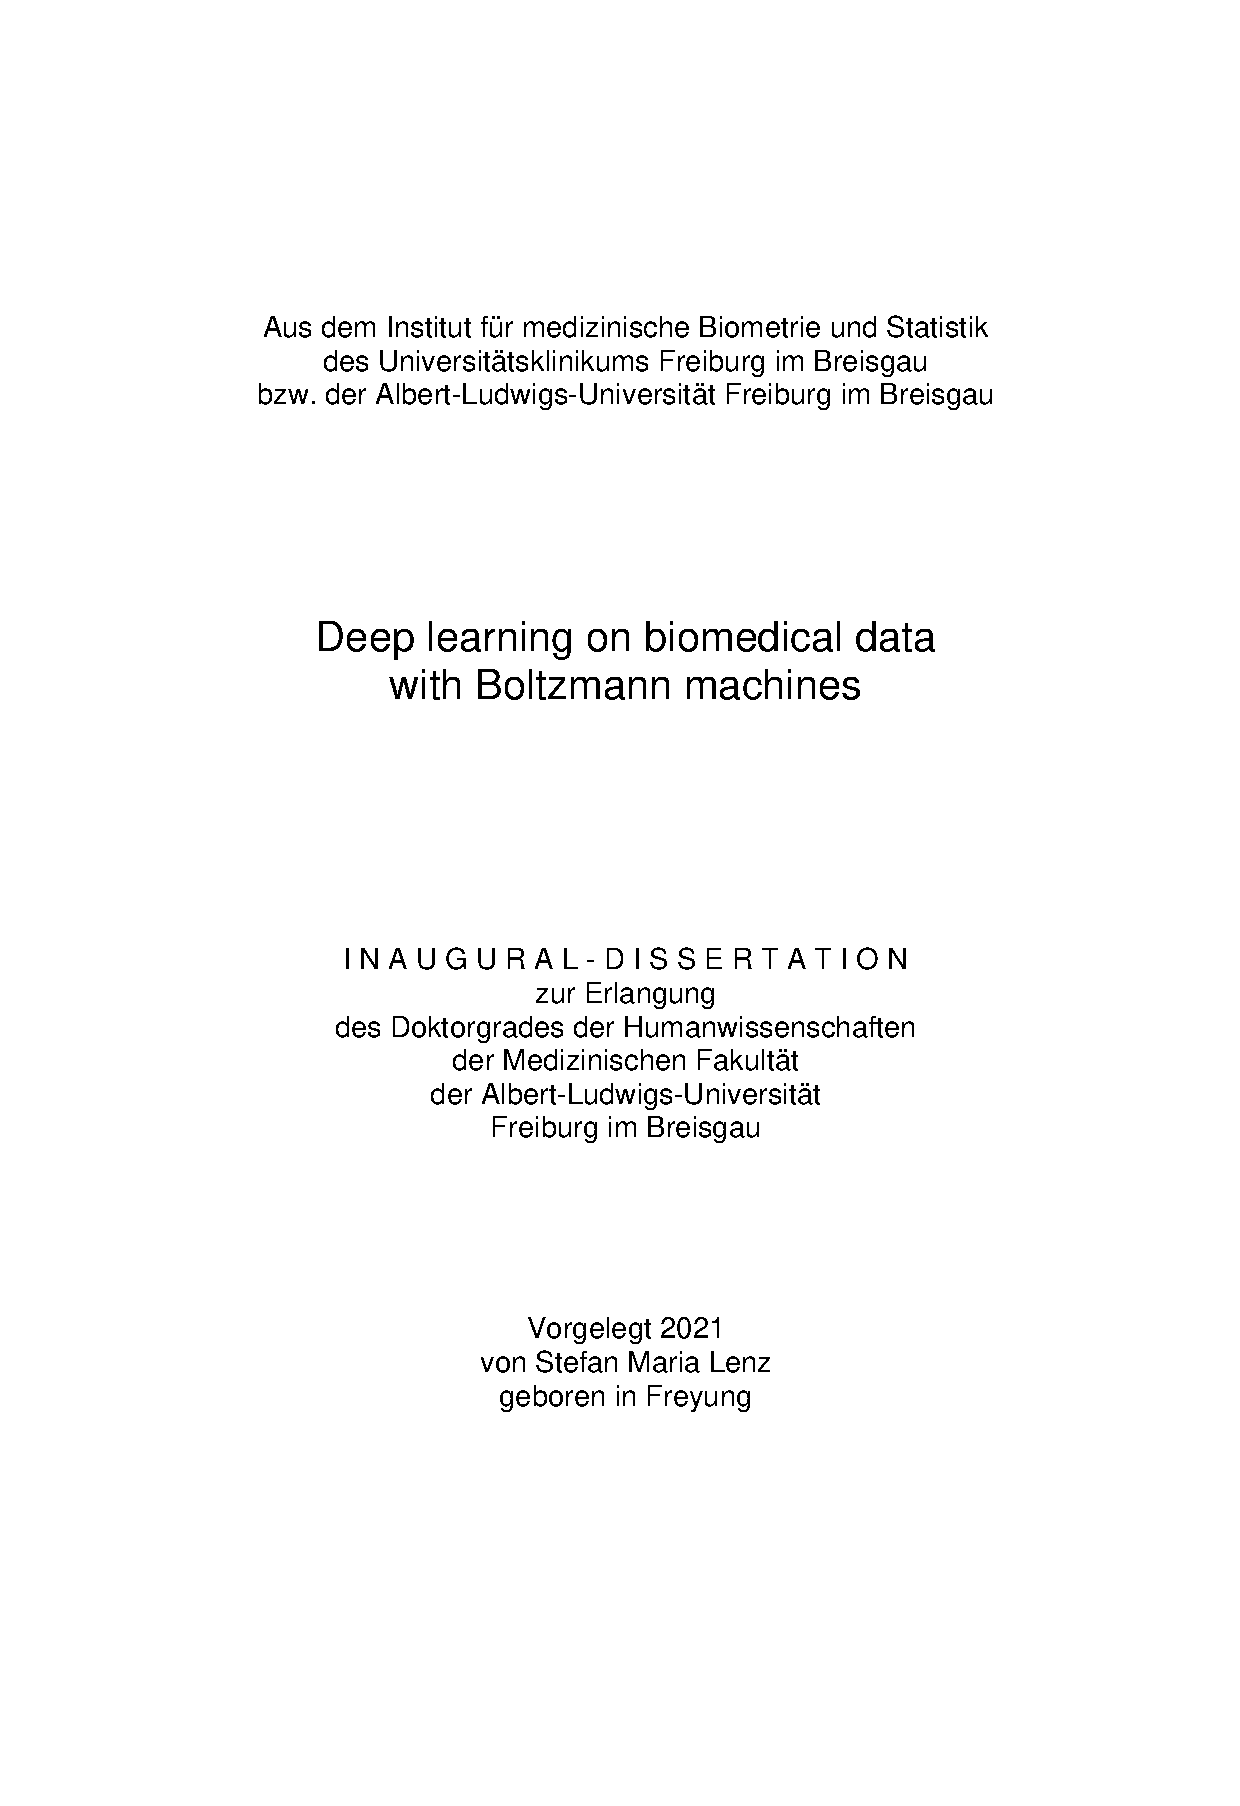
\includepdf[pages=-]{includes/Deckblatt}

%\maketitle

\tableofcontents
\newpage
\onehalfspacing
\setlength{\emergencystretch}{3em}
\selectlanguage{english}

\section*{Abstract}

%But since these data sets can be very heterogeneous compared to the widely used image data, the choice of hyperparameters for training is especially challenging.
%Therefore the package puts a strong focus on monitoring and evaluating the learning process.
%Primary evaluation criterion is the likelihood of the model, which can be estimated using annealed importance sampling (AIS). We present our approach for adapting the AIS algorithm on multimodal deep Boltzmann machines in detail in the article.
%Additionally to likelihood estimation, this package offers convenience methods to monitor a number of other statistics and it allows to easily extend the monitoring of the training.

Deep Boltzmann machines (DBMs) are considered as a promising approach for deep learning on data of small sample size, which is common in biomedical data sets.
To make DBMs available for experimentation, an easily extensible implementation of DBMs was created in form \apkg{BoltzmannMachines} Julia package, which has been registered in the official Julia package repository.
The implementation offers several unique features, in particular for evaluation and monitoring of the training of DBMs.
This is especially important for biomedical data sets, where finding good hyperparameters is hard due to the diversity of the data.

In addition to small sample sizes, data protection constraints may impose an additional challenge for analyzing biomedical data, in particular, if the data is distributed across different sites and cannot be pooled for the analysis.
One approach for conducting privacy-preserving analyses in such a setting is to generate synthetic data, which captures the important structure of the original data of the individuals and, at the same time, can be used with less data protection constraints as the original data.
For this, DBMs are compared with other popular generative approaches, namely generative adversarial networks (GANs) and variational autoencoders (VAEs) with respect to generative performance and disclosure risk.
In addition to these neural network approaches, simpler methods such as multiple imputation by chained equations (MICE) and independent marginals (IM) are also considered as references.
The experiments show the feasibility of DBMs as a generative approach in distributed settings, even with small sample sizes at different sites.
VAEs showed also a comparable performance to DBMs in this setting, while the other approaches performed considerably worse.

Finally, a ready-to-use implementation for DBMs as distributed approach is presented.
This software is built in form of R packages that integrate into the DataSHIELD infrastructure, which provides a framework for conducting privacy-preserving analyses on distributed cohorts.
Since DataSHIELD is based on the R programming language, and there is no DBM implementation in R, a language interface was necessary to bring the functionality of the \apkg{BoltzmannMachines} package to R.
There are two existing packages, \apkg{JuliaCall} and \apkg{XRJulia} that also make it possible to connect R with Julia, but they did not offer all necessary features.
Therefore, a new solution was created, which provides convenient interactive handling and, at the same time, puts a special focus on the stability that is needed for a production environment.
The resulting \apkg{JuliaConnectoR} R package has been officially registered in the Comprehensive R Archive Network (CRAN).
More generally, this approach of wrapping external deep learning functionality proves also on the technical side that advanced deep learning algorithms can be used for distributed privacy-preserving analyses in DataSHIELD.


\clearpage
\section{Introduction}

Deep learning algorithms have revolutionized image and speech recognition \citep{goodfellow_deep_2016}, and are the state-of-the-art in many fields for prediction models.
Also advances in bioinformatics have been made using deep learning.
Yet, there are some challenges that prevent deep learning from being used in bioinformatics applications. 

One particularly big challenge is limited data \citep{min_deep_2017}.
While the amount of data in fields such as image and speech recognition has been increased dramatically with the content available in the internet, the amount of usable genetic or medical data remains comparatively small.
The problem of small sample sizes is particularly prevalent when dealing with genetic variant data
because there is a high number of genetic variants, and, at the same time, the sequencing of genomes is still relatively expensive.
This results in relatively few samples compared to the number of dimensions in data sets of genetic variants.
Also for clinical data, the availability of high-quality data is one of the key challenges \citep{machine_learning_review_nejm}.
Although there is an abundance of routine care data, sample sizes are often small when it comes to curated data or data from clinical studies.
Additionally, privacy restrictions make it difficult to use health information of humans for research and further limit the amount of accessible data.
For example, the European General Data Protection Regulation (GDPR) requires an explicit consent for analyzing the health care data of individuals, which makes it hard to collect large amounts of data that can be used for various research purposes \citep{rumbold_effect_2017}.
Thus, approaches that can yield good results with only a limited amount of data are needed in many cases when applying deep learning on biomedical data.

Unsupervised learning is particularly interesting if there is not enough or no labeled data.
In contrast to prediction models, which require labeled data as input, unsupervised learning techniques aim at capturing structure of the input data without a specific prediction task.
One class of unsupervised deep learning approaches are {\em generative models}, which are able to generate new data according to a distribution that is learned from input data \citep{sejnowski_unsupervised_1999}.
Generative models have made their appearance in mainstream media when an artist trained a generative model on images of paintings, used it to create new paintings, and sold one of these paintings for \$432,000 at the auction house Christie's \citep{cohn_ai_2018}.
The generative approach used there is called generative adversarial network (GAN) \citep{goodfellow_generative_2014}.
Other generative approaches in the field of deep learning are variational autoencoders (VAEs) \citep{Kingma2013} and deep Boltzmann machines (DBMs) \citep{salakhutdinov2009DBMs}.
In a comparison of GANs, VAEs, and DBMs on genetic variant data of different rather small sample sizes, DBMs showed a good generative performance \citep{nussberger_synthetic_2020}.
Besides generating data, DBMs and VAEs can be used for dimensionality reduction by analysing the activation in higher-level layers of the network, which encode features of increasing complexity in the data.
This has, e.g., been applied to find patterns in gene expression data \citep{ding_interpretable_2018, hess_exploring_2020}.

Another possible application of generative models is to create synthetic data for privacy-preserving analyses.
Synthetic data is data that has similar properties to original data but that is not linked to individual samples of the original data.
In the same way as the previously mentioned generated paintings are not simply modified versions of original paintings but entirely new fabrications,
synthetic patient data is not created from single patients but from the distribution of patient characteristics that have been learned by a generative model.
The advantage of synthetic data is that it can be used with less data protection restrictions of the original data as it does not contain individual-level data.
This can be useful in settings where data is distributed and sharing the data of individuals is prohibited due to privacy concerns.
For example, in the MIRACUM consortium \citep{prokosch_miracum_2018}, which includes ten German University hospitals,
one of the goals is to jointly analyze data that is distributed across multiple sites.
However, pooling the data of all patients for joint analysis is not possible because of data protection laws.
Therefore, alternative ways of analyzing the data must be sought. 
One way to conduct analyses across distributed data is provided by the DataSHIELD software \citep{gaye_datashield,budin-ljosne_datashield}.
This has been used in several multicenter projects conducting epidemiological studies \citep{doiron_datashield_2013, pastorino_datashield_2019, oluwagbemigun_datashield_2020}.
With DataSHIELD, many common statistical analyses can be conducted.
Generating synthetic data in DataSHIELD has also already been explored for enabling analyses that were previously not possible \citep{bonofiglio2020}.
The question is here, whether deep learning techniques can also be brought to DataSHIELD for creating synthetic data, and whether they pose an increased risk with respect to violations of privacy.

%Multimodal DBMs have been used by Srivastava et al. for image captions \citep{srivastava2012multimodal}.
%Here we want to broaden the scope a little bit and present an extensible approach for creating deep Boltzmann architectures with different types of visible units and flexible partitioned hidden layers. Training of such architectures ....
%Those architectures are not only useful for putting data of different types in one model but also in cases where a natural partitioning of the data can be derived from domain knowledge. With partitioning one can greatly reduce the number of parameters in the model. This allows training models on data sets where the sample size would otherwise be too small to fit a full model.

%Idee: aus motivation von Bioinf App not fail: VAE and GAN backpropagation, DBMs harder to train and the algorithm is complex.

%Idee: DBMs multimodal , e. g. clinical, gene expression, and single nucleotide polymorphism (SNP) data

Unsupervised learning is also called self-supervised learning if the model is designed to predict parts of the input from other parts \citep{lecun_selfsupervised_2019}.
One advantage of DBMs is that it is particularly easy to perform such predictions of parts of data based on other parts.
This can be achieved via conditional sampling, i.e., drawing from the learned distribution conditioned on certain values of input variables \citep{salakhutdinov2015generativemodels}.
The flexibility in conditional sampling separates DBMs from VAEs and GANs, where this is not possible.
Variants of VAEs and GANs have been proposed for this, called {\em conditional VAEs} \citep{cvae} and {\em conditional GANs} \citep{cgan}.
The latter has also been applied to gene expression data \citep{wang_conditional_2018}.
There, the prediction of gene activation from so-called landmark genes, which are suspected to contain most information of the genome, has been improved.
For this, and in conditional VAEs and conditional GANs in general, the variables that are used as conditions need to be specified in the training.
DBMs have the advantage that the specification of specific variables as conditions is not necessary and conditions can be set on arbitrary variables.
Conditional sampling in DBMs could therefore be used to simulate the regulation of arbitrary gene expression patterns based on a DBM model that has been trained on genetic expression data.
Such a model that has learned the overall structure of a data set is then also able to utilize the information about the whole distribution when making inferences about smaller subgroups.

Apparently deep Boltzmann machines exhibit promising qualities for deep learning on biomedical data, where limited sample size and privacy restrictions are common challenges.
An additional big challenge for deep learning on biomedical data is finding good hyperparameters for the optimization algorithms \citep{min_deep_2017}.
Since biomedical data sets can be very diverse, default values for hyperparameters may often not be the best choice and the ability to determine good hyperparameters is especially important there.
As the success of the learning depends critically on good hyperparameters, a special emphasis needs to be put on evaluating the learning.

This work aims to investigate how DBMs can be used to tackle the challenges for deep learning on biomedical data. Furthermore, it strives to make DBMs accessible in form of user-friendly software.

In a first step, the algorithms for training and evaluating DBMs need to be implemented in a way that is suitable for experimentation (Section \ref{bmpart}).
This implementation can then be used to examine the hypothesis that DBMs can produce useful synthetic data in scenarios with small sample size and also with distributed data (Section \ref{simuexp} and Section \ref{realexp}).
For employing DBMs in settings with sensitive health information, the disclosure risk of synthetic data created by DBMs must be investigated as well.
After this, DBMs can be considered for generating synthetic data in the DataSHIELD infrastructure.
Since DataSHIELD is based on the R programming language, the algorithms for training and evaluating DBMs must also be made available in R (Section \ref{juliaconnectorpart}).
Finally, a solution for applying DBMs via DataSHIELD can be provided (Section \ref{dsBoltzmannMachinesImpl}).


\clearpage
\section{Deep Boltzmann machines}\label{bmpart}
\subsection{Theoretical background}\label{bmtheory}

Boltzmann machines \citep{ackley_boltzmann_1985} are a special kind of neural networks.
Artificial neural networks have been developed for solving complex problems by imitating structures of the nervous system of humans and animals \citep{mcculloch_logical_1943}.
Boltzmann machines have been derived from models in statistical physics, which have some interesting parallels with networks of neurons.

In physics, Ising models aim at modeling the magnetic spin in lattices of atoms or molecules in ferromagnetic crystals \citep{isingmodel}.
In Ising models models the probability of the magnetic spin of molecules in a lattice of molecules is determined by an energy function that assigns an energy to each possible configuration of magnetic spins in the lattice.
Configurations with a lower energy have a higher probability of occurring.
This connection between energy and and probability holds also for Boltzmann machines.
It makes Boltzmann machines a type of so-called ``energy-based" models \citep{ranzato_ebm}.

The analogy of lattices of molecules with magnetic spin are networks of neurons in the nervous system, where each cell may have a neural activation.
The analogy goes further.
Neural networks receive input from data in special nodes.
The information about the data can then be learned by the network.
In the physics analogue, this corresponds to parts of the lattice that are influenced by an external magnetic field.
In both cases, the information about the input is encapsulated in the parameters of the model, which influence the energy function and thereby determine the probability of the activations in the network.
With the information contained in the model parameters, a trained Boltzmann machine can be used for generating new samples according to the distribution that the model has learned from the original data.
With this ability, Boltzmann machines can be employed as {\em generative models}.

The following parts of this section give an overview of the mathematical definitions surrounding Boltzmann machines that will be necessary to understand how Boltzmann machines can be trained and used.
This also includes the definition of some terminology that is commonly used in the literature about Boltzmann machines.

\subsubsection{Definition of Boltzmann machines}\label{basicbmproperties}

A Boltzmann machine model with parameters $\Theta$ defines a probability distribution $p(x)$ for a random variable $x = (v, h)$ on a probability space $\Omega$ via the energy function $E(v, h; \Theta)$:
\begin{equation}
   p(x) = p(v, h) = \frac{e^{-E(v,h)}}{Z}.
   \label{eqn:probbm}
\end{equation}
The normalizing factor $Z$, the so called \emph{partition function}, is defined as $Z = \int_{\Omega} e^{-E(x)} dx$.
In case of a discrete probability distribution, this can be written as $Z = \sum_{v,h}e^{-E(v,h)}$ where the sum goes over all possible realizations of $v$ and $h$.
The term in the denominator $p^*(v,h) = e^{-E(v,h)}$ is called \emph{unnormalized probability}.
The probability space can be divided into dimensions of observed variables (subsumed in vector $v$) and hidden/latent variables (in $h$), corresponding to visible and hidden nodes in the graphical representation, see Figure \ref{fig:bmsoverview}.

The so called \emph{free energy}, a notation also inspired by physics, is defined as
\[
   F(v) = - \log \sum_h e^{-E(v, h)}.
\]
With this definition, we can rewrite the formula of the partition function as $Z = \sum_v e^{-F(v)}$.
That is useful because the formula for the free energy of restricted Boltzmann machines can be simplified by using the layerwise structure (see e.g.~\cite{martens_representational_2013}, appendix A.1).
Thus the complexity of calculating the free energy becomes linear in the number of hidden nodes, as can be seen in the formulas for the free energy in the different types of models that are described below.
If the partition function $Z$ is given, the log-likelihood
\begin{equation}
   \log p(v) = - F(v) - \log Z
\label{eqn:pRBMfreeenergy}
\end{equation}

can therefore be calculated efficiently using the free energy. The free energy is also used for calculating unnormalized probabilities $p^*(v) = e^{-F(v)}$, which is, e.g., used in the annealed importance sampling algorithm (see \ref{methodAIS}) for estimating the partition function via a stochastic algorithm.

With these basic properties defined, we can go further to take a look at the details of specific types of Boltzmann machines.
Here only the special cases of restricted Boltzmann machines and (multimodal) deep Boltzmann machines are considered.
These models have restrictions on their parameterization compared to a general Boltzmann machine.
The restrictions correspond to a layered design of their graphs.
For an intuitive overview of the architectures of the different types that are considered here, see Figure \ref{fig:bmsoverview}.

\begin{figure}[h]

   \centering
   
\includegraphics[scale=3.]{images/BMsOverview.eps}
   \caption{Graph view on different types of Boltzmann machines. Visible units (i. e. input units) are depicted as nodes with doubled circle lines. Hidden units are simple circles.
 {\bf A}: General Boltzmann machine, with all nodes connected to each other. {\bf B}: Restricted Boltzmann machine (RBM). Each of the lines corresponds to a weight, i.e. an entry in the weight matrix $W$, like in formulas (\ref{eqn:energyformularbm}) and (\ref{eqn:energyformulagbrbm}).
{\bf C}: Deep Boltzmann machine. From a graph perspective, this is simply a stack of RBMs.
{\bf D} and {\bf E}: Multimodal/partitioned deep Boltzmann machines. In a multimodal DBM, the different partitions of the visible nodes may also have different distributions.}
   \label{fig:bmsoverview}
 \end{figure}


\subsubsection{Basic properties of restricted Boltzmann machines}\label{rbmtypes}

\emph{Restricted Boltzmann machines} \citep{smolensky1986foundations}, or RBMs,  consist of two layers, a visible layer $v$, which receives the input data, and a hidden layer $h$, which encodes latent features of the data. For a graphical depiction, see Figure \ref{fig:bmsoverview}B.
The nodes, also called ``units'' in neural network terminology, play the role of neurons.
The nodes are divided into several layers.
The nodes inside the same layer are not connected to each other, and therefore, the network has the form of a bipartite graph \citep{diestelgraph}.
Although other distributions are also possible for the hidden nodes \citep{hinton_practical_2012}, only RBMs with binary hidden nodes following a Bernoulli distribution are considered here.
The types of RBMs presented in the following may, however, differ in the distribution of their visible nodes, which makes them suitable for modeling different types of input data.

\paragraph{Bernoulli distributed visible nodes}
The most basic model in this class of models are restricted Boltzmann machines with Bernoulli distributed nodes, most of the time simply called restricted Boltzmann machines. Their energy function is of the form
\begin{equation}
   E(v,h) = - a^T v - b^T h - v^T W h. \label{eqn:energyformularbm}
\end{equation}

The parameters of the model are $\theta = (W, a, b)$ with \emph{weight matrix} $W$, vector $a$ as the \emph{visible bias}, and $b$ as the \emph{hidden bias}.
The weights correspond to the connections between the visible and hidden units in a weighted graph, as shown in Figure \ref{fig:bmsoverview}.
The bias variables are usually not depicted in graph views of neural networks, but they are equivalent to adding nodes to the model that always have the value one. The visible bias corresponds to the weights of the connections to an additional node that is connected to all nodes of the visible layer, and the hidden bias corresponds to the weights of the connections to an additional node that is connected to all nodes of the hidden layer. The bias variables serve to set a basic level of activation of the nodes, which is then modified by the input from the connected units.
To see the mapping from the parameters in the formula to the network view, see Figure \ref{fig:rbmweights}.

\begin{figure}[h]
   \centering
   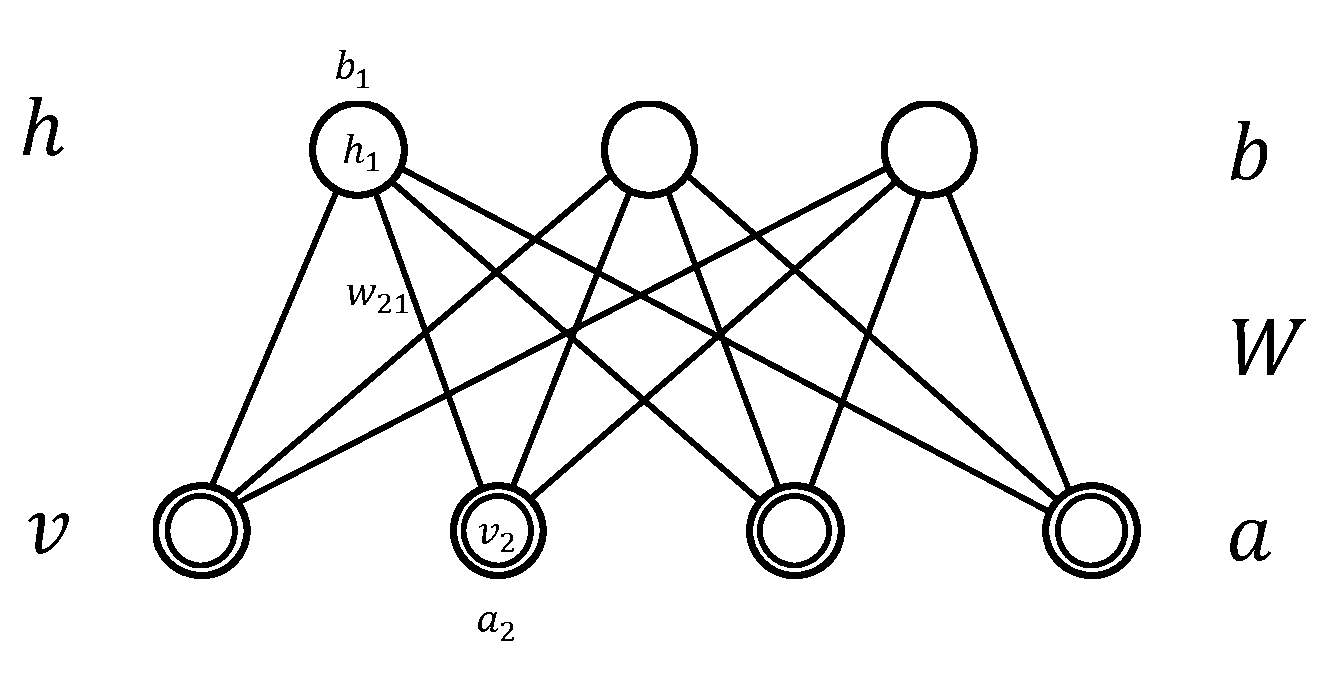
\includegraphics[scale=0.5]{images/rbmweights.pdf}
   \caption{The nodes and parameters of a restricted Boltzmann machine in the graph view. The second visible node and the first node in the hidden layer are connected with weight $w_{21}$ from the weight matrix $W$. The base-level activity of the nodes $v_2$ and $h_1$ is determined by the biases $a_2$ and $b_1$, respectively.}
   \label{fig:rbmweights}
 \end{figure}


The formulas for the conditional distributions $p(h | v)$ and $p(v | h)$ can be derived from (\ref{eqn:energyformularbm}). (For a detailed derivation see, e.g., \cite{krizhevsky2009tinyimagesthesis}, Section 1.4).
Employing the sigmoid function $\sigm(x) = \frac{1}{1+ e^{-x}}$, the resulting conditional distributions can be written as
\begin{equation}
p(v_i | h) = \sigm ((a + W h)_i)
 \quad \text{and}\quad
p(h_i | v) = \sigm ((b + W^T v)_i).
\label{eqn:condprobrbm}
\end{equation}

The free energy is
\begin{equation}
F(v) = - a^T v - \sum_{j=1}^{n_H} \log \left (1 + e^{(W^T v + b)_j}\right).
\label{eqn:freenergy_rbm}
\end{equation}

The trick for deriving the formula of the free energy is to ``analytically sum out" the hidden units \citep{sala2012anefficient}.
The master thesis of \cite{krizhevsky2009tinyimagesthesis} is a very good resource for looking up the complete derivations of these formulas. This holds not only for the theory of RBMs with Bernoulli distributed nodes but also in particular for RBMs with Gaussian distributed visible nodes, which are presented next.

\paragraph{Gaussian distributed visible nodes}\label{gaussianrbm}
One approach for modeling continuous values for $v$ are restricted Boltzmann machines with Gaussian distributions of the visible variables and Bernoulli distributed hidden variables. \cite{krizhevsky2009tinyimagesthesis} defines the energy of the model  as:
\begin{equation}
   E(v,h) = \sum_{i=1}^{n_V}\frac{(v_i - a_i)^2}{2\sigma_i^2} - b^T h - \sum_{i=1}^{n_V} \sum_{j=1}^{n_H} \frac{v_i w_{ij} h_j}{\sigma_i}
   \label{eqn:energyformulagbrbm}
\end{equation}

The number of visible and hidden nodes is denoted as $n_V$ and $n_H$, respectively. The parameters of this model are $\theta = (W, a, b, \sigma)$ with weight matrix $W$, visible bias $a$ hidden bias $b$ and standard deviation $\sigma$. The role of $\sigma$ as standard deviation becomes clearer by looking at the conditional distributions of the $v_i$ given $h$, which are distributed according to the normal distribution $\mathcal{N}(a_i + \sigma_i(Wh)_i, \sigma_i^2)$. For the hidden nodes, one can show that $p(h_j | v) = \sigm \left (b_j + \sum_{i=1}^{n_V} w_{ij} \frac{v_i}{\sigma_i} \right )$.
The free energy is
\begin{equation}
   F(v) = \sum_{i=1}^{n_V}\frac{(v_i - a_i)^2}{2\sigma_i^2} + \sum_{j=1}^{n_H} \log \left (1 + e^{b_j + \sum_{i=1}^{n_V} \frac{v_i}{\sigma_i} w_{ij}} \right)
\label{eqn:freenergy_gbrbm}
\end{equation}
\citep{krizhevsky2009tinyimagesthesis}.

\cite{cho2011improved} proposed a different parameterization for the energy function to improve the training of RBMs with Gaussian visible nodes:
\begin{equation}
   E(v,h) = \sum_{i=1}^{n_V}\frac{(v_i - a_i)^2}{2\sigma_i^2} - b^T h - \sum_{i=1}^{n_V} \sum_{j=1}^{n_H} \frac{v_i w_{ij} h_j}{\sigma_i^2}
   \label{eqn:energyformulagbrbm2}
\end{equation}
In this model the distribution of the visible nodes $v$ conditioned on the hidden nodes $h$ is the multimodal normal distribution $\mathcal{N}(a + Wh, \sigma^2)$.
The conditional distribution of the hidden nodes is $p(h_j | v) = \sigm \left (b_j + \sum_{i=1}^{n_V} w_{ij} \frac{v_i}{\sigma_i^2} \right )$, and the free energy is
\begin{equation*}
   F(v) = \sum_{i=1}^{n_V}\frac{(v_i - a_i)^2}{2\sigma_i^2} + \sum_{j=1}^{n_H} \log \left (1 + e^{b_j + \sum_{i=1}^{n_V} \frac{v_i}{\sigma_i^2} w_{ij}} \right).
\end{equation*}

%TODO cite:
%\citep{melchior_gbrbm}, \citep{cho_gaussiandbm}
% TODO mention alternative: use continuous as Gaussian hard., verweis auf entsprechenden results teil


\subsubsection{Gibbs sampling in restricted Boltzmann machines}\label{gibbssamplingrbm}
In the previous sections concerning RBMs with different input distributions, one could see that it was possible to specify a formula for the conditional probability that has the same  algorithmic complexity of the matrix multiplication in all cases.
However, the formula for the simple probability $p(v)$ of a sample $v$ requires calculating the partition function $Z$ (see formula (\ref{eqn:probbm})), and calculating $Z$ is not feasible for most practical scenarios, as the number of summands in $Z$ grows exponentially with the number of nodes in the model (see also later in \ref{methodExactloglik}).
This means that using RBMs as generative models, i.e. drawing samples according to the distribution captured in its parameters, is not as straightforward as calculating $p(v)$ and sampling according to the distribution.

But because of the layered structure of RBMs and the closed form of the conditional distributions $p(v \mid h)$ and $p(h \mid v)$, which is fast to evaluate, it becomes possible to efficiently apply a Markov chain Monte Carlo technique called \emph{Gibbs sampling} \citep{gibbssamplingorig} for approximating the distribution of the RBM.
The Gibbs sampling  algorithm for RBMs can be formulated as follows:

\begin{enumerate}
\item Start with an arbitrary $v_1$.
\item Draw $h_1$ according to $p(h \mid v_1)$.
\item Draw $v_2$ according to $p(v \mid h_1)$.
\item Repeat steps 2 and 3 until convergence.
\item Result: After $n$ steps, $v_n$ and $h_n$ have been drawn according to the joint distribution $p(v,h)$ of the model.
\end{enumerate}

This works because the iteration forms a Markov chain that has the distribution $p(v,h)$ of the model as its equilibrium distribution.

\paragraph{Conditional sampling}\label{condsamplingrbm}
The Gibbs sampling algorithm can also be easily modified for sampling conditionally on the activations of input nodes by clamping the activations of the nodes that are to be conditioned on and running the Gibbs sampling algorithm in the rest of the network.
Put more formally, to draw from the probability $p(v, h \mid \tilde{v}_C)$ that is conditioned on the activations $\tilde{v}_C$ of a set $C$ of visible nodes, the Gibbs sampling algorithm above can be run with $v_C$ set to $\tilde{v}_C$ in step 1 and after each sampling step 3.
This, of course, works analogously for hidden nodes as conditions.


\subsubsection{Training of restricted Boltzmann machines}\label{rbmtraining}
Goal of the training procedure of restricted Boltzmann machines is to maximize the likelihood $\prod_{k=1}^n p(\widetilde{v}^{(k)})$ for a given data set $(\widetilde{v}^{(1)}, \dots, \widetilde{v}^{(n)})$.
Maximizing the likelihood is equal to maximizing the log-likelihood
\[
\sum_{k=1}^{n}  \log p(\widetilde{v}^{(i)}) = \sum_{k=1}^{n} \left( \log \sum_h e^{-E(\widetilde{v}^{(k)}, h)} - \log \sum_v \sum_h e^{-E(v, h)} \right).
\]


\paragraph{Deriving the gradient of the log-likelihood}

For finding an optimum for $\sum_{k=1}^{n}  \log p_\Theta(\widetilde{v}^{(k)})$, the gradient $\nabla_\Theta \sum_{k=1}^{n}  \log p_\Theta(\widetilde{v}^{(k)})$ needs to be determined.
The gradient of the log-likelihood for a single observation
$\widetilde{v} $ with respect to the parameter set $\Theta$ is
\begin{align}
\nabla_{\!\Theta}  \log p(\widetilde{v}) &= \nabla_{\!\Theta}   \log \sum_h e^{-E(\widetilde{v}, h)} - \log \sum_v \sum_h e^{-E(v, h)} \nonumber \\
 &= \frac{\nabla_{\!\Theta} \sum_h e^{-E(\widetilde{v}, h)}}{\sum_h e ^{-E(\widetilde{v}, h)}} - \frac{\nabla_{\!\Theta} \sum_v \sum_h e^{-E(v,h)}}{\sum_v \sum_h e^{-E(v,h)}} \label{eqn:derivedlog}\\
&=  \frac{\sum_h e^{-E(\widetilde{v}, h)} \nabla_{\!\Theta} (-E(\widetilde{v}, h))} {\sum_h e^{-E(\widetilde{v}, h)}} - \frac{\sum_v \sum_h e^{-E(v, h)} \nabla_{\!\Theta} (-E(v, h))}{\sum_v \sum_h e^{-E(v, h)}} \label{eqn:derivedexp}\\
&=  \EX_{P_\text{data}} \nabla_{\!\Theta} (- E(\widetilde{v},h)) - \EX_{P_\text{model}} \nabla_{\!\Theta} (-E(v,h)) \label{eqn:nablaresult}
\end{align}
In (\ref{eqn:derivedlog}) and (\ref{eqn:derivedexp}), the chain rule is used, together with the derivative of the logarithm and the exponential function, respectively. The resulting terms can be rewritten in (\ref{eqn:nablaresult}) as the expectation of the gradient given the distribution of the data and the expectation of the gradient given the distribution of the model.

As can be seen in Equation (\ref{eqn:derivedexp}), the calculation of the gradient involves sums over lots of possible combinations of activations of nodes.
The first term can be calculated in the types of RBMs that have been introducted here.
For this, one can use the expected value of the conditional probability $p(h\mid\widetilde{v})$ and plug it in:
\begin{equation}
\EX_{P_\text{data}} \nabla_{\!\Theta} E(\widetilde{v},h) =  \nabla_{\!\Theta} E(\widetilde{v}, \EX(p(h \mid \widetilde{v}))
\label{eqn:plugexpectedh}
\end{equation}
In the second term of Equation (\ref{eqn:nablaresult}), the sum goes over all nodes in the network.
Calculating this term is technically not feasible in normal cases, as the number of summands grows exponentially with the number of nodes.
This means that it is not possible to simply equate the gradient of the log-likelihood with zero and solve the equation to get an optimum. Also finding an optimum with gradient descent \citep{gradientdescent}, walking with small steps in the direction of the gradient to find an optimum, is not possible directly, because this would as well require the calculation of the whole gradient in each iteration step.
Via Gibbs sampling (see Section \ref{gibbssamplingrbm}), however, the term can be estimated.
With this, it becomes possible to use the estimated gradients in gradient descent, or here rather ``gradient ascent" as we would like to find a (local) maximum.

\paragraph{Batch gradient optimization and the role of mini-batches}

For the practical implementation, another stochastic approximation of the gradient for the full data set $\sum_{k=1}^n \log p(\widetilde{v}^{(k)})$ is used.
Usually a form of {\em batch gradient optimization} \citep{bottou_optimization_2018} is performed.
For this, the samples are split into batches $B_l$, usually of approximately equal sizes $b_l$.
In each optimization step $t$, the parameters are updated as follows:
\[
\Theta^{(t+1)} = \Theta^{(t)} + \frac{\epsilon}{b_l} \sum_{\widetilde{v} \in B_l} \nabla_{\!\Theta^{(t)}} \log p(\widetilde{v})
\]

The step size is determined by the {\em learning rate} $\epsilon$.
Each iteration $t$ calculates the gradient of a different batch $B_l$ until all samples have been used.
The mini-batches are usually reused multiple times for the learning.
The number of steps after all samples/mini-batches are used for updating the parameters, is called a {\em (training) epoch}.
(In the formula above one training epoch is over if $t = \sum_l b_l$.)
Training usually consists of many epochs and the step size is kept small, e.g. a hundred epochs and a learning rate of 0.001 could be a viable combination.
The number of epochs and the learning rate are the most important hyperparameters for the training.

%TODO optional: hier könnte man mehr schreiben über zusammenspiel von learning rate und epochs, außerdem steps auf oberfläche beschreiben und learning rate decay

Mini-batches were at first introduced for performance reasons.
It is not necessary to have the exact gradient for walking only small steps into the direction of it.
So it is sufficient to calculate the gradient for small subsets of the data, which is noisy, but will be correct on average.
Using mini-batches can also be advantageous because of another reason: The variance of the steps becomes higher with a with a smaller batch size. This leads to exploring more of the surface of the likelihood function in the high-dimensional space and therefore can lead to finding better local optima in some scenarios \citep{bengio2012practical}.

\paragraph{Contrastive divergence}

For performing batch gradient optimization, the Gibbs sampling procedure is also modified for RBM training to speed up the learning process.
In other applications, thousands of iterations are used for Gibbs sampling  \citep{gibbssamplingorig}. For training RBMs, a shortcut is used, which is called {\em contrastive divergence} (CD) \citep{cdorig, perpinan_contrastive_2005}.
In CD, the number of Gibbs sampling steps is reduced drastically. In most cases, even only one step is used, which is denoted with $\text{CD}_1$ \citep{hinton_practical_2012}.
Instead of using a random starting point, CD uses the original sample $\widetilde{v}$, for which the gradient shall be computed, as starting point $v_1$ of the sampling procedure. This should ensure that the starting point is already close to the desired distribution.

Another modification of the Gibbs sampling procedure used for training of RBMs is {\em persistent contrastive divergence} (PCD).
Similar to CD, this procedure also uses only very few steps. Here, the state of the Gibbs sampling chain for calculating the last update is reused and used as starting point. \cite{hinton_practical_2012} recommends PCD over $\text{CD}_1$ or even $\text{CD}_{10}$.

\paragraph{Gradients for different types of restricted Boltzmann machines}\label{rbmgradients}

In an RBM with Bernoulli distributed nodes, Equation (\ref{eqn:nablaresult}) leads to the following formulas for the gradients for the weights and biases:
\begin{align*}
\frac{\partial}{\partial W}  \log p(\widetilde{v}) &= \EX_{P_\text{data}}  \widetilde{v}^T h - \EX_{P_\text{model}} v^T h \\
\frac{\partial}{\partial a}  \log p(\widetilde{v}) &=  \EX_{P_\text{data}}
\widetilde{v} - \EX_{P_\text{model}}  v = \widetilde{v} - \EX_{P_\text{model}} v\\
\frac{\partial}{\partial b}  \log p(\widetilde{v}) &=  \EX_{P_\text{data}} h - \EX_{P_\text{model}} h
\end{align*}

In an RBM with Gaussian visible nodes \citep{krizhevsky2009tinyimagesthesis}, the  gradients are:
\begin{align*}
\frac{\partial}{\partial W} \log p(\widetilde{v}) &= \frac{1}{\sigma_i} \left ( \EX_{P_\text{data}} \widetilde{v}^T h - \EX_{P_\text{model}} v^T h \right) \\
\frac{\partial}{\partial a} \log p(\widetilde{v}) &= \frac{1}{\sigma_i^2} \left(\widetilde{v} - \EX_{P_\text{model}} v \right)\\
\frac{\partial}{\partial b} \log p(\widetilde{v}) &= \EX_{P_\text{data}} h - \EX_{P_\text{model}} h \\
\frac{\partial}{\partial \sigma_{i}} \log p(\widetilde{v}) &= \EX_{P_\text{data}} \left( \frac{(\widetilde{v}_i - a_i)^2}{\sigma_i^3} - \sum_{j=1}^{n_H} h_j \frac{w_{ij} \widetilde{v}_i}{\sigma_i^2}\right) \\ & \quad \quad - \EX_{P_\text{model}} \left(\frac{(v_i - a_i)^2}{\sigma_i^3} -\sum_{j=1}^{n_H} h_j \frac{w_{ij} v_i}{\sigma_i^2} \right)
\end{align*}

In the alternative formulation of \cite{cho2011improved}, the gradients are:
\begin{align*}
\frac{\partial}{\partial W} \log p(\widetilde{v}) &= \frac{1}{\sigma_i^2} \left ( \EX_{P_\text{data}} \widetilde{v}^T h - \EX_{P_\text{model}} v^T h \right) \\
\frac{\partial}{\partial a} \log p(\widetilde{v}) &= \frac{1}{\sigma_i^2} \left(\widetilde{v} - \EX_{P_\text{model}} v \right)\\
\frac{\partial}{\partial b} \log p(\widetilde{v}) &= \EX_{P_\text{data}} h - \EX_{P_\text{model}} h \\
\frac{\partial}{\partial \sigma_{i}} \log p(\widetilde{v}) &=  \frac{1}{\sigma_i^3} \Bigg( \EX_{P_\text{data}} \left( (\widetilde{v}_i - a_i)^2 - 2\sum_{j=1}^{n_H} h_j w_{ij} \widetilde{v}_i  \right) \\ & \quad \quad - \EX_{P_\text{model}} \left((v_i - a_i)^2 -2\sum_{j=1}^{n_H} h_j w_{ij} v_i \right) \Bigg)
\end{align*}

In the RBM with the dummy variables for encoding categorical variables, the gradients are the same as in the one with Bernoulli distributed variables.

Using the gradients specified above, it is possible to run the gradient optimization for training the different types of RBMs.

\subsubsection{Deep belief networks}\label{dbns}

The next step in the evolution deep Boltzmann machines are deep belief networks (DBNs) \citep{hinton_reducing_2006}, which have been invented to make better use of RBMs for dimensionality reduction.
Detecting higher level features in data is hard using shallow networks such as RBMs.
The idea of DBNs is to stack RBMs on top of each other (see Figure \ref{fig:dbn}) to be able to model features of increasing complexity with an increased depth of the network.

\begin{figure}[h]
   \centering
   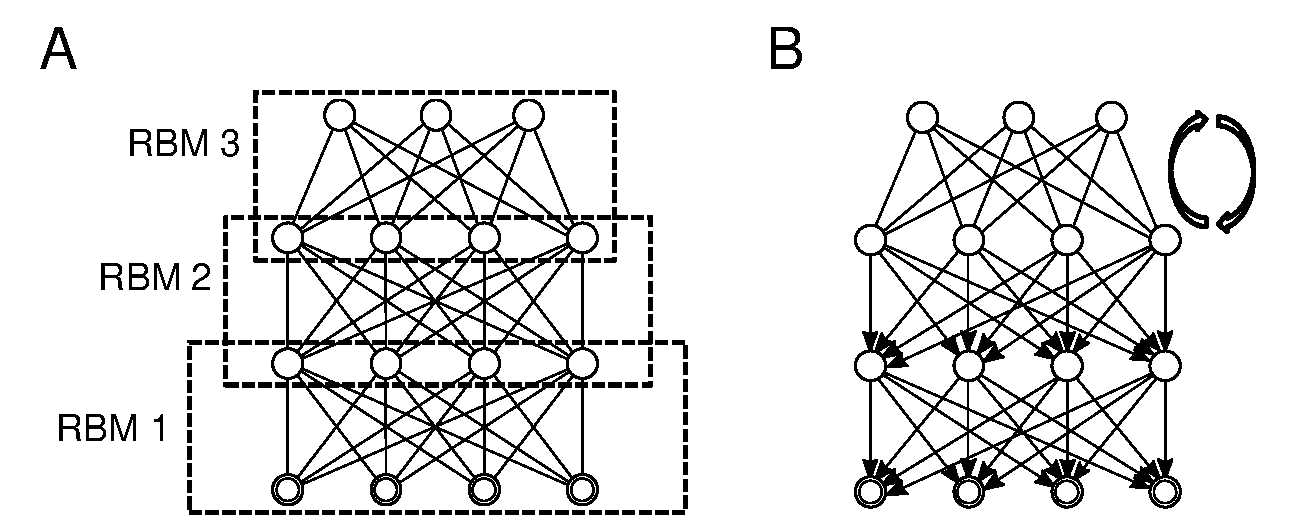
\includegraphics[scale=0.7]{images/dbn.pdf}
   \caption{Training a deep belief network (DBN) and using it as generative model.
   {\bf A}: The DBN is trained as a stack of RBMs. {\bf B}: In a DBN as generative model, only the top RBM is used for Gibbs sampling, then the activation is passed in a deterministic way downwards to the visible layer.}
   \label{fig:dbn}
 \end{figure}

For training a DBN, the first RBM is trained with the original data data vectors $\tilde{v}^{(i)}$ with $i = 1, \dots, n$.
For training the higher layers, a deterministic activation $f_k(v) :=  \EX p_k(h|v)$, defined via the conditional probability in the $k$-th RBM model, is passed through the lower layers after they have been trained:
The second RBM is trained with the data set of all $f_1(\tilde{v}^{(i)})$, the third RBM can then be trained with the data set $f_2(f_1(\tilde{v}^{(i)}))$, and so on.

As shown in figure (\ref{fig:dbn}B), only the last RBM in the network can be used for sampling, which limits the generative capabilities of a DBN.
The ability to generate data from complex distributions is furthermore reduced if the DBN is used for dimension reduction because in this case the top RBM is also the smallest network.


\subsubsection{Deep Boltzmann machines}\label{dbmprobs}

If the network architecture of a DBN is treated as a Boltzmann machine, we get a \emph{deep Boltzmann machine}, where the complete network can be utilized for generating samples.
A deep Boltzmann machine, as defined by \cite{salakhutdinov2009DBMs}, with $n_L$ number of hidden layers has parameters
\[
\Theta = \left (W^{(1)}, \dots, W^{(n_L)}, a, b^{(1)}, \dots, b^{(n_L)} \right).
\]
The energy is defined as
\[
E(v, h^{(1)}, \dots, h^{(n_L)}) = - a^T v - v^T W^{(1)} h^{(1)} - \sum_{k=1}^{n_L} b^{(k)} h^{(k)} -  \sum_{k=2}^{n_L} h^{(k-1)}W^{(k)}h^{(k)}.
\]
For the connection between the formula and the resulting network architecture see Figure \ref{fig:dbmweights}.
\begin{figure}[h]
   \centering
   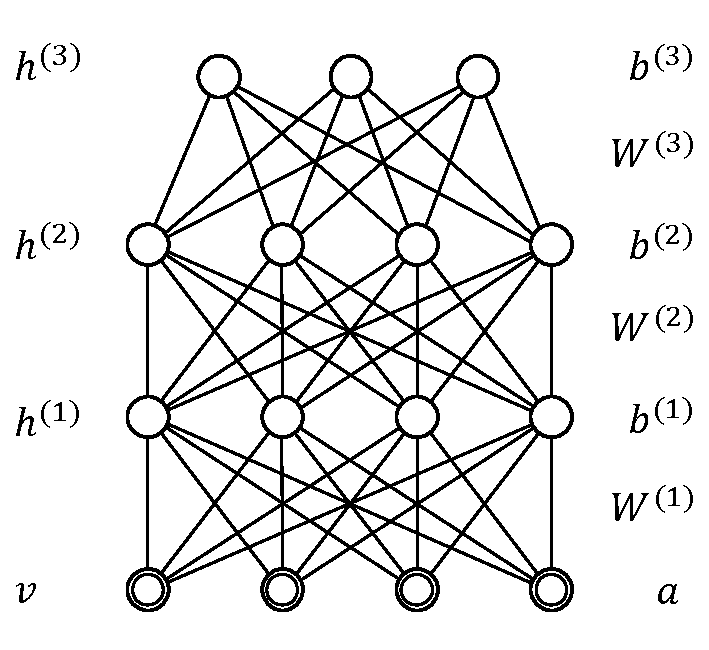
\includegraphics[scale=0.6]{images/dbmweights.pdf}
   \caption{The nodes and parameters of a deep Boltzmann machine in the graph view}
   \label{fig:dbmweights}
 \end{figure}

A deep Boltzmann machine has Bernoulli distributed nodes.
Due to the layer-wise structure, the conditional probability of the visible nodes $p(v \mid h) = p(v \mid h^{(1)})$ depends only on the first hidden layer and can be calculated like in an RBM with Bernoulli distributed nodes.
The conditional probability of the final hidden layer $p \left( h^{n_L} \mid v, h^{(1)}, \dots, h^{(n_L -1)} \right) = p \left( h^{n_L} \mid h^{(n_L -1)} \right)$ can similarly be calculated by knowing only on $h^{(n_L-1)}$.
For the intermediate layers, the conditional probability can be calculated if the neighboring layers are given as
\begin{equation}
p\left(h^{(1)} \mid v, h^{(3)}\right) = \sigm \bigg( b^{(1)} + (W^{(1)})^T v + W^{(3)} h^{(3)} \bigg)
\label{dbmcondprobfirsthidden}
\end{equation}
for the first hidden layer and
\begin{equation}
p\left(h^{(k)} \mid h^{(k-1)}, h^{(k+1)} \right) = \sigm \bigg( b^{(k)} + (W^{(k-1)})^T h^{(k-1)} + W^{(k+1)} h^{(k+1)} \bigg)
\label{dbmcondprobintermediate}
\end{equation}
for all other intermediate hidden layers.

These conditional probabilities can be used to perform Gibbs sampling in deep Boltzmann machines (see Figure \ref{fig:dbmsampling}) similar to the Gibbs sampling algorithm in restricted Boltzmann machines (as described before in \ref{condsamplingrbm}).

\begin{figure}[h]
   \centering
   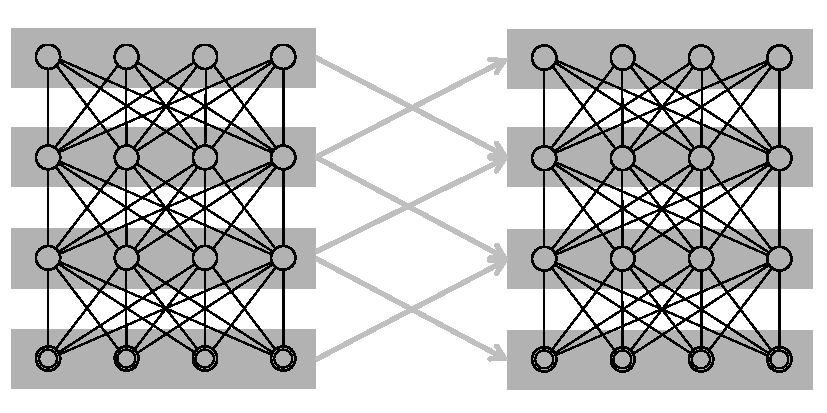
\includegraphics[scale=1.0]{images/dbmsampling.pdf}
   \caption{Gibbs sampling step in a deep Boltzmann machine. The visible layer is sampled using only the activation of the first hidden layer from the previous Gibbs sampling step, and the last hidden layer is sampled using only the activation of the penultimate hidden layer. The intermediate layers are sampled by using the activations of the two neighboring layers from the previous Gibbs sampling step. }
   \label{fig:dbmsampling}
 \end{figure}


\subsubsection{Training of deep Boltzmann machines}\label{dbmtraining}


In context of DBMs, the DBN learning algorithm (see \ref{dbns}) is called greedy layerwise pre-training.
This pre-training helps the algorithm for training a general Boltzmann machine to find a better optimum.
An intermediate layer in a DBM receives input from its neighboring layers (see formula (\ref{dbmcondprobintermediate}) and Figure \ref{fig:dbmsampling}), but during pre-training it only gets input from the layer below. To account for this, the DBN training is modified for training a DBM and the input from the visible layer ($ = (W^{(1)})^T v$) and from the last hidden layer (= $W^{(n_L-1)} h^{(n_L)}$) is doubled.
\citep{salakhutdinov2009DBMs}.


Using the pre-trained DBM as starting point, the fine-tuning of the weights can then be performed by the algorithm for training a general Boltzmann machine
\citep{salakhutdinov2009DBMs, salakhutdinov2015generativemodels}.
This algorithm is also based on gradient descent.
In RBMs it is possible to calculate $p(h | v)$ because all the hidden nodes are only depending on the visible nodes.
This allowed to calculate $\EX_{P_{\text{data}}} \nabla_{\!\Theta} E(\tilde{v},h)$ from $\EX p(h | \tilde{v})$ (see formula (\ref{eqn:plugexpectedh})).
In DBMs this is not possible any more as the hidden layers are connected with each other and therefore no simple formula for $p(h | v)$ can be derived.
This means that calculating the derivative of the log-likelihood in deep Boltzmann machines needs an additional technique.
\cite{salakhutdinov2009DBMs} propose a variational approach for this.
The true distribution $p(h|v)$  is replaced with an approximation $q(h|v)$.
Instead of optimizing the log-likelihood, a lower bound is optimized, for which the gradient can be computed.
This \emph{variational lower bound} or \emph{evidence lower bound} (ELBO) \citep{blei_variational_2017} for the likelihood is
\[
\log p(v) \geq \sum_h q(h|v) \log p(v,h) + \mathcal{H}(q)
\]
$\mathcal{H}(q)$ denotes the entropy of the distribution $q$.
Here a ``mean-field approximation" $q$ is used, where all hidden nodes are assumed to be independent.
The distribution is then $q(h) = \prod_{k=1}^{n_L} \prod_j^{n_{H,k}} q(h_i^{(k)})$ with $q(h_i^{(k)} = 1) = \mu_i^{(k)}$ for some fixed values $\mu_i^{(k)}$ for each  node $i$ in a hidden layer $k$.
($n_L$ denotes the number of hidden layers and $n_{H,k}$ the number of nodes in hidden layer $k$.)
This leads to the lower bound of the log-likelihood, which will be optimized in the fine-tuning algorithm: %TODO ableiten? steht in sala learning deep generative models equation 36
\[
   \log p(v) \geq - E(v, \mu) - \log Z + \mathcal{H}(q) =: \ELBO(v, \mu)
\]
$E$ is the energy in the DBM and $\mathcal{H}(q) = \sum_j \left( \mu_j \log \mu_j + (1- \mu_j) \log ( 1- \mu_j) \right)$ is the entropy of $q$ \citep{sala2012anefficient, salakhutdinov2015generativemodels}.

To calculate $\mu$ for a given data vector $\tilde{v}$, the following equations for a fix-point iteration can be used, which are analogous to formulas (\ref{dbmcondprobfirsthidden}) and (\ref{dbmcondprobintermediate}).
\begin{align*}
\mu^{(1)}(t+1)&= \sigm \bigg( b^{(1)} + (W^{(1)})^T \tilde{v} + W^{(2)} \mu ^{(2)}(t) \bigg) \\
\mu^{(k)}(t+1) &= \sigm \bigg( b^{(k)} + (W^{(k)})^T \mu^{(k-1)}(t) + W^{(k+1)} \mu^{(k+1)}(t) \bigg) \\
&\quad\quad (\text{for} \; k=2,\dots, n_L-1) \\
\mu^{(n_L)}(t+1)&= \sigm \bigg( b^{(n_L)} + (W^{(n_L)})^T \mu^{(n_L-1)}(t) \bigg)
\end{align*}
For  $t \rightarrow \infty$, the series $\mu(t)$ converges to the value of $\mu$ that can be used for calculating the gradient for the lower bound.
As a starting value for $\mu$, activation in the network is induced by the input using a single forward pass, treating the DBM as a DBN (see \ref{dbns}).

Analogously to equation (\ref{eqn:nablaresult}) for calculating the gradient of the log-likelihood in RBMs, the gradient of the variational lower bound of the log-likelihood can be calculated as
\begin{align*}
\nabla_{\Theta} \ELBO(v, \mu) &= \nabla_{\Theta} ( - E(\tilde{v}, \mu) - \log Z ) \\
 &= \nabla_{\Theta} (- E(\tilde{v}, \mu)) - \EX_{P_\text{model}} \nabla_{\Theta} (-E(v, h)).
\end{align*}
This results in the following gradients for the different types of model parameters:
\begin{align*}
\frac{\partial}{\partial W^{(1)}} \ELBO(\tilde{v}, \mu) &= \widetilde{v}^T \mu - \EX_{P_\text{model}} v^T h^{(1)} \\
\frac{\partial}{\partial W^{(k)}} \ELBO(\tilde{v}, \mu) &= (\mu^{(k-1)})^T \mu^{(k)}  - \EX_{P_\text{model}} (h^{(k-1)})^T h^{(k)} &\quad(k = 1, \dots, n_L)\\
\frac{\partial}{\partial a}  \ELBO(\tilde{v}, \mu) &=  \widetilde{v} - \EX_{P_\text{model}}  v \\
\frac{\partial}{\partial b^{(k)}}  \ELBO(\tilde{v}, \mu) &=  \mu^{(k)} - \EX_{P_\text{model}} h^{(k)}  &\quad ( k = 1, \dots, n_L)
\end{align*}

The expected values under the distribution of the model ($\EX_{P_\text{model}}$) are estimated like in the RBM by running a Gibbs sampler (see Figure \ref{fig:dbmsampling}).
This Gibbs sampler is run with a number of parallel persistent chains, which are called ``fantasy particles" \citep{salakhutdinov2009DBMs}. The results are averaged over the number of fantasy particles to get better estimations for the expected values in the distribution of the model.
For the convergence of the gradient optimization, it is necessary to decrease the learning rate $\epsilon_t$ over time such that the series $\sum_{k=1}^\infty \epsilon_t^2$ converges, e.g. $\epsilon_t = \frac{c}{d+t}$ with constants $c, d > 0$ \citep{sala2012anefficient}.

Since the training procedure is very complex and depends on many hyperparameters, it is necessary to test whether the training works well by examining the training objective.
Although the likelihood is not the best criterion for all kinds of applications \citep{theis_note_2015}, it is essential to have a way to get a value for the likelihood as primary optimization criterion.
Being able to inspect the learning process is important for finding the best choice of hyperparameters and also for ensuring the quality of the software implementation of the learning algorithm.
This leads us to the next section, where we want to take a closer look at methods for calculating and estimating the likelihood, and the lower bound of the likelihood, in case of DBMs.


\subsubsection{Evaluating restricted and deep Boltzmann machines}
A special challenge for unsupervised learning on non-image data in general is the lack of performance indicators.
In supervised training, the classification accuracy is the natural evaluation criterion, which is also easy to implement.
In unsupervised training with a well investigated class of data such as images, there is already much experience available for choosing the model architecture and the hyperparameters. If models are to be trained on very diverse data, the problem of finding good hyperparameters is exacerbated as parameter tuning can pose a different challenge for each data set.

Thus the need for having an objective evaluation criterion as a basis for choosing the hyperparameters and monitoring the training becomes very important.
In case of images or natural language, the generative abilities of a model can be tested by simply looking at the generated images or sentences to see whether these are proper samples. In the case of data from a patient record or genetic data, this approach is not feasible.

If there are no other evaluation criteria, one indicator for successful learning in Boltzmann machines remains the model likelihood, which is an inherent property of the model and is therefore applicable in all cases of data. The difficulty for calculating the likelihood is its dependency on the partition function (see formula (\ref{eqn:probbm})).
In most cases, the likelihood cannot be calculated exactly but it can only be estimated by stochastic algorithms like annealed importance sampling (AIS).
% So we also want to detail the extension of AIS on multimodal deep Boltzmann machines in this article.

\paragraph{Exact calculation of the partition function}
\label{methodExactloglik}
As mentioned in Section \ref{rbmtraining}, the exact calculation of partition functions is only computationally feasible for very small models as its complexity grows exponentially. Exploiting the layerwise structure allows a faster exact calculation of $Z$ such that the computation time does not grow exponentially with the number of all nodes but only grows exponentially with the number of elements in a subset of the nodes. It is possible to utilize the formula for the free energy in restricted Boltzmann machines (see formulas (\ref{eqn:freenergy_rbm}) and (\ref{eqn:freenergy_gbrbm})), where the hidden layer is summed out analytically.
With this it is possible to reduce the number of summands.
The complexity for calculating the partition function for all the different types of  models described here is then still $\mathcal{O}(2^n)$, but with an $n$ smaller than the number of nodes:

By using the formulas for the free energy and the symmetry of restricted Boltzmann with binary nodes, $n = \min(n_V, n_H)$ with $n_V$.
In RBMs with one of layer Gaussian nodes and one layer of binary nodes, $n$ is the number of binary nodes, since the contribution of the Gaussian nodes can be integrated analytically.
In case of a deep Boltzmann machine, it is possible to sum out each second layer, similar to the calculation of the free energy in restricted Boltzmann machines. So for DBMs, $n$ can be reduced to the number of nodes in each second layer, see Figure \ref{aissummingout}.

\begin{figure}[h!]
\centering
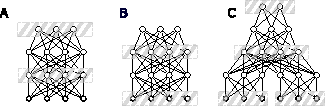
\includegraphics[scale=2.5]{images/AISsummingout.pdf}
\caption{Possibilities for summing out layers for calculating the likelihood. For calculating the likelihood in a more efficient way, the layers in the gray boxes can be summed out analytically. {\bf A:} Summing out the odd layers in this DBM leaves $2^{(4 + 4)} = 256$ summands that still have to be summed in order to calculate the likelihood. {\bf B:} Summing out the even layers in this DBM leaves in $2^{(4 + 3)} = 128$ summands. {\bf C:} Summing out the even layers in  this multimodal DBM leaves $2^{(6 + 3)} = 512$ summands.}
\label{aissummingout}
\end{figure}

\paragraph{Estimating partition functions with annealed importance sampling (AIS)}\label{methodAIS}

For annealed importance sampling we need a sequence of intermediate distributions
$p_0, \dots p_K$ with
$p_0 = p_A$ and $p_K = p_B$. The ratio $\frac{Z_B}{Z_A}$ is then estimated by the mean of a number of so called {\em importance weights} that are determined as
\[
   \prod_{k=1}^K \frac{p^*_k(x^{(k)})}{p^*_{k-1}(x^{(k)})}.
\]
Each of the importance weights is an estimator for $\frac{Z_B}{Z_A}$.
To get an estimation of this fraction with less variance, the mean all the importance weights is used to estimate  $\frac{Z_B}{Z_A}$.
The $x^{(k)}$ are produced by iteratively performing Gibbs sampling. Starting with $x_0$ sampled from $p_0$, one obtains $x^{(k)}$ by sampling a Gibbs chain that is initialized with $x^{(k-1)}$ in an intermediate model with distribution $p_k$. An appropriate choice for the intermediate models are Boltzmann machines with the energy functions $E_k$ chosen such that
\[
   E_k(x) = (1 - \beta_k) E_A(x) + \beta_k E_B(x)
\]
and therefore
\[
   p_k^*(x) = p_A^*(x)^{1-\beta_k} p_B^*(x)^{\beta_k}.
\]
The factors $\beta_k$ with $0 = \beta_0 < \beta_1 < ... < \beta_K = 1$ are called temperatures \citep{salakhutdinov2008learning}.
The choice of the temperatures, the number of importance weights and also the number of Gibbs sampling steps for the transition are hyperparameters for the AIS algorithm.

With AIS it is possible to get a direct estimate of the partition function $Z_A$ of a model $A$ by annealing from the model $A$ to a null model with all weights being zero as model $B$.
$Z_A$ can be computed from the estimation of $\frac{Z_B}{Z_A}$ because the partition function $Z_B$ of the null model can be calculated exactly. This approach is shown in Figure \ref{figTwotypesais}A.

It is also possible to compare the likelihood of two models instead of calculating it directly.
For this, only the ratio $\frac{Z_B}{Z_A}$ between two full models needs to be estimated.
There are two practical approaches for constructing intermediate models  for directly annealing from one full model to another full model (see also Figure \ref{figTwotypesais}, B and C):
\begin{enumerate}
\item Combining (adding) corresponding weights of two models of the same size to get an intermediate model of the same size.
\item Constructing a larger model by putting the two models next to each other and connecting their nodes, increasing the energy in one part of the combined model while reducing it in the other part \citep{theis2011deepbelief}:
\end{enumerate}
\begin{figure}[h!]
\centering
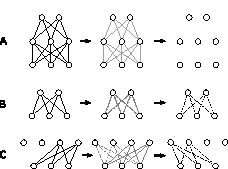
\includegraphics[scale=3.5]{images/twotypesais.pdf}
\caption{Different approaches for performing AIS.
The tempered weights of the intermediate distributions are shown in grey. Black lines correspond to the original weights of a model. No lines between nodes are equal to the weights being zero.
{\bf A:} Annealing from a null model, where all weights are zero, to the full model.
{\bf B:} Annealing from one RBM model with three visible nodes and two hidden nodes to another model of the same size.
The weights of the first model are depicted as continuous lines, the weights of the second as dashed lines. Here, model one is gradually morphed into model two. {\bf C:}
The same two RBMs are compared again by annealing from a model that is equivalent to the first model to a model that is equivalent to a second model via a combined, bigger model. For this approach, both models do not necessarily have to be of the same size.}
\label{figTwotypesais}
\end{figure}
The approach with a combined model (see Figure \ref{figTwotypesais}C) is more flexible and allows to estimate the ratios of two arbitrary Boltzmann machines of the same type and with the same number of hidden nodes.
But it requires sampling in a Boltzmann machine that has as many hidden nodes as the two models together.

In a DBM, it is possible to use only the states of each second layer from samples generated by running a Gibbs chain \citep{salakhutdinov2008learning}. The unnormalized probabilities of these states can be calculated by analytically summing out the other layers.
For this, we can use the fact that the states in one layer are independent from the states of each non-adjacent layer to get the unnormalized probability $p_k^*(\tilde{h})$ for the subset $\tilde{h} = \left(h^{(1)}, h^{(3)}, \dots\right)$ of a generated sample $x = \left( v, h^{(1)}, h^{(2)}, \dots \right)$ in an intermediate model.
The layers that can be analytically summed out are the same as the ones shown in Figure \ref{aissummingout}.
To calculate the ratio $\frac{p_k^*(x_k)}{p_{k-1}^*(x_{k})}$, one can derive the formula for $p^*(\tilde{h})$ in a DBM similarly to the free energy $F(v) = - \log p^*(v)$ in RBMs \citep{sala2012anefficient}. For a DBM with three hidden layers, the formula is
\begin{align}
p^*( \tilde{h} ) =&  e^{(b^{(1)})^T h^{(1)}} \prod_j (1+ \exp((a + W^{(1)} h^{(1)})_j)) \; \cdot \nonumber \\
&e^{(b^{(3)})^T h^{(3)}} \prod_{j}  \left( 1 + \exp \left( (b^{(2)} + (W^{(2)})^T h^{(1)} + W^{(3)} h^{(3)})_j \right) \right).
\label{eqn:aisunnormalizedprob}
\end{align}

Here the visible layer $v$ and the second hidden layer $h^{(2)}$ have been summed out analytically, like shown in Figure \ref{aissummingout}B.

%Note that the model for Gibbs sampling, used as the Markov transition operator, can differ from the model that is used to evaluate the unnormalized probability $p_k^*(h)$ as long as the probability distribution $p_k(h)$ of the hidden nodes is the same.
%This trick can be used to fit AIS for GBRBMs in the same schema as RBMs with Bernoulli distributed nodes.


It can be noted that the term in the first line of formula \ref{eqn:aisunnormalizedprob} is equal to the unnormalized probability of the hidden nodes in a RBM with Bernoulli distributed nodes.
This procedure can be generalized for AIS on multimodal DBMs.
If we have the unnormalized probability $p^*(h)$ for each type of RBM that receives the data input, it becomes possible to calculate the unnormalized probability of sampled hidden values in a multimodal DBM in the same way as for a standard DBM with only Bernoulli distributed nodes.
The formula for the unnormalized probability for the respective RBM type (see Section \ref{unnormalizedprobsrbm}) can then be used for summing out the visible units in formula \ref{eqn:aisunnormalizedprob} by substituting the term in the first line with the product of the unnormalized probabilities for all RBMs in the visible layer.

The formulas for $p^*(h)$ for each different type of RBM are derived next, also by analytically ``summing out", or in case of Gaussian RBMs, ``integrating out" the visible layer.


\paragraph{Calculating or estimating likelihoods in deep Boltzmann machines}
For a restricted Boltzmann machine, the likelihood can be calculated using formula (\ref{eqn:pRBMfreeenergy}) if the partition function is known. This is not so easily possible in a DBM, for which calculating the distribution of the hidden nodes is of exponential complexity.
Estimating the likelihood of DBMs is possible using AIS by constructing a smaller DBM for each sample and estimating its partition function.
The smaller DBM is constructed by removing the visible layer, and incorporating contribution of the sample to the energy of the first RBM - consisting only of visible and first hidden layer - into the bias of the new visible layer which was the first hidden layer of the original model.
The partition function of this smaller model is then the unnormalized probability of the sample in the original model.
In a setting with very large sample size, the cost of estimating the actual likelihood with this procedure is too expensive. But if the sample size is small enough, it is affordable to estimate the likelihood and not fall back on the lower bound.

\paragraph{Alternatives to the likelihood for RBMs}
The AIS algorithm is very complex to implement.
It is also compute-intensive, depending on the required exactness of the estimation.
So often there are other statistics used for checking the training progress.

The free energy cannot be used for comparing different models because it does not include the normalization by $Z$.
It can, however, be used to compare how well the same model fits different data sets.
One application for this is monitoring the overfitting by comparing the training data set and a test data set \citep{hinton_practical_2012}.
\label{reconstructionerror}
Another popular statistics, which behaves similar to the likelihood in RBMs in most cases, is the {\em reconstruction error} \citep{hinton_practical_2012}.
For defining this, one needs at first to define the term {\em reconstruction} in an RBM.
The reconstruction \citep{hinton_practical_2012} for a sample $\widetilde{v}$ is calculated by using the conditional probabilities as deterministic ``activation potential".
With $f_h(h) := \EX_v p(h|v)$ and $f_v(h) := \EX_h p(v|h)$, the reconstruction $r(v)$ can be defined as $r(\widetilde{v}) := f_v(f_h(\widetilde{v}))$. The reconstruction error is then the distance between the sample $\widetilde{v}$ and its reconstruction $r(\widetilde{v})$, e.g. measured as absolute distance or quadratic distance.

Calculating the reconstruction error  is a very fast and simple technique for monitoring the training progress for RBMs, DBNs and for greedy layer-wise pre-training of DBMs.
Although the reconstruction error can serve as a rough proxy statistic for the likelihood, it does not replace the likelihood entirely, as it is not the actual optimization target, and it is strongly influenced by the {\em mixing rate} of the Markov chain for Gibbs sampling, i. e. how fast the Markov chain reaches its equilibrium distribution. If the distribution in the Markov chain changes very slowly, the reconstruction error will be low, even if the distributions of the samples and the model differ much \citep{hinton_practical_2012}.

\subsubsection{Multimodal deep Boltzmann machines}

Figure \ref{fig:bmsoverview} shows different possible architectures for multimodal Boltzmann machines \citep{srivastava2012multimodal}.
Multimodal DBMs can be considered a generalization of DBMs.
They have been invented to make it possible to combine different input data types in a single model.

The training procedure of multimodal DBMs can be generalized as follows:
For the pre-training of a multimodal DBM, the different layers are trained by stacking RBMs in the same way as for pre-training a DBM.
The only differences are that the RBMs at the lowest layer may have different input distributions, and that RBMs in higher layers may be partitioned, i.e., some connections are always zero.
For the fine-tuning, the gradients in the different layers are calculated in the same way as the gradients in the respective RBM types, using the mean-field approximations and the fantasy particles of the DBM fine-tuning algorithm as activations of the respective visible and hidden nodes.
Gibbs sampling can also be performed in the same way, using the conditional probabilities in the RBMs.


\subsection{Theoretical developments}\label{bmaddtheory}

\subsubsection{A new approach for modeling categorical data}\label{methodsoftmax0}
%TODO auch beschreiben, dass man bernoulli und categoriale variablen in einem haben kann
Another important statistical data type that needs to be handled when dealing with biomedical data is data with categorical values.
For most applications in machine learning, categorical data is usually encoded in dummy variables \citep{hastie_elements}.
It would be possible to use the binary dummy variables as input to a restricted or deep Boltzmann machine with Bernoulli distributed visible units as well.
But when sampling from such a Boltzmann machine model all combinations of visible nodes have a positive probability. This can be seen from the formula of the conditional probability (\ref{eqn:condprobrbm}) and the fact that the values of the sigmoid function are strictly positive.
Therefore, the resulting data is not properly encoded in general  because illegal combinations of dummy variables can occur. With that, sampled values cannot be mapped to the original categories any more.
Using dummy variables as input to Boltzmann machines with Bernoulli distributed variables makes it also more difficult to learn higher level patterns, as the Boltzmann machine has at first to learn the pattern that results from the dummy encoding  by itself. Hence it is advised to use a Boltzmann machine that has the knowledge about the encoding built into its energy function and probability distribution.


For encoding categorical variables, the most popular encoding used by the machine learning frameworks \apkg{TensorFlow} \citep{tensorflow}, \apkg{scikit-learn} \citep{scikit-learn} or \apkg{Flux} \citep{flux} is the so-called ``one-hot encoding", which encodes a variable with $k$ categories in a binary vector of $k$ components, where exactly one component is one and all others are zero.
An advantage of this is that all categories are treated equally.
Here, I tried a slightly different variant.
A categorical variable with $k$ categories is encoded in $k-1$ binary dummy variables.
For example, this is the encoding of the values for a variable with four categories:

\begin{table}[h!]
\centering
\begin{tabular}{cc}
Categorical value & Dummy encoding \\
\hline
1 & 0 0 0 \\
2 & 1 0 0 \\
3 & 0 1 0 \\
4 & 0 0 1 \\
\end{tabular}
\caption{Dummy encoding with reference category for a categorical variable with four categories}\label{dummenc}
\end{table}

This variant is the technique for creating dummy variables for categorical variables in regression models \citep{faraway_regression}.
One category is used as reference category for the interpretation of the regression coefficients.
This allows to be parsimonious with parameters.
As already pointed out in the introduction, this may therefore help with deep learning on genetic data in particular.
Consider genetic variant data that contains values 0/1/2 for each of defined location on the human genome to encode that there is no deviation from the reference genome (0), a deviation on one chromosome (1) or a deviation on both chromosomes (2).
An RBM receiving input with dummy encoding using the natural reference category 0 needs only two thirds of the parameters that an RBM needs which receives the same data in one-hot encoding.

The energy function $E$ for RBMs with categorical data is the same as for Bernoulli distributed visible nodes (see formula \ref{eqn:energyformularbm}).
The difference is that not all combinations of visible nodes are allowed. Thus the partition function $Z = \sum_{v} \sum_{h} e^{-E(v,h)}$ and the probability
$p(v) = \frac{\sum_h e^{-E(v,h)}}{Z}$ change because the sum over all possible states of $v$ in the formula for $Z$ contains less summands than in the case with a Bernoulli distribution, where all combinations of activations are possible.

For deriving the formulas for an RBM that handles the dummy encoding like exemplified in Table \ref{dummenc}, let us denote with $C_k$ the set of dummy variables that the dummy variable $k$ belongs to.
The visible nodes of the RBM can cover multiple categorical variables and multiple sets of dummy variables, which may differ in the number of categories.
If the number of categories equals two for all categorical variables, this model is the same as an RBM with Bernoulli distributed nodes.

Like \cite{krizhevsky2009tinyimagesthesis} let us write $E(v_k = 1, v_{i \neq k}, h)$ for the energy of the combination of a visible vector $v$ with $v_k = 1$ and a hidden vector $h$. Similarly, let us define $E(v_{i \in C_k} = 0, v_{i \notin C_k}, h)$ for the energy of the combination of a visible vector $v$ that is zero in all dummy variables that belong to $C_k$ and a hidden vector $h$.

From the previously defined dummy encoding results that if one dummy variable in the set is one, all others in the set are zero.
The sum over all possible combinations of $v$ can therefore be split into those parts where a dummy variable $k$ is zero and one part where all others in the corresponding set of dummy variables are one, because these covers all allowed combinations.
This allows to split the formula for the unnormalized probability of the hidden nodes into the following sum:
\begin{align}
p^*(h) &= \sum_v  \exp (-E(v,h)) \nonumber \\
&= \sum_{v_{i \notin C_k}} \exp (-E(v_{i \in C_k} = 0, v_{i \notin C_k}, h)) + \sum_{c \in C_k} \sum_{v_{i \notin C_k}} \exp ( - E(v_c = 1, v_{i \notin C_k},  h))
%E(v_k=1, v_{i\neq k}, h) = E(v_k = 1, v_{i \notin C_k}, h).
\end{align}

The input from the hidden nodes can further be extracted from $ \sum_{v_{i \notin C_k}} e^{-E(v_{k=1}, v_{i \neq k}, h)}$ by regrouping the summands:
\begin{align}
&\sum_{v_{i \notin C_k}} \exp ( - E(v_c = 1, v_{i \notin C_k},  h)) = \nonumber \\
&\quad = \sum_{v_{i \notin C_k}} \exp \left( \sum_{i \notin C_k} v_i h_j w_{ij} + \sum_{i \notin C_k} a_i v_i + a_k  + \sum_j h_j w_{kj} +\sum_j h_j b_j \right) \nonumber \\
&\quad = \exp \left( (Wh)_k + a_k \right) \sum_{v_{i \notin C_k}} \exp \left(-E(v_{i \in C_k} = 0, v_{i \notin C_k}, h) \right)
\label{eqn:sumvksoftmax}
\end{align}

The unnormalized probability $p^*(h)$ of the hidden nodes can now be rewritten as:

\begin{align}
p^*(h) =& \sum_{v_{i \notin C_k}} \exp (-E(v_{i \in C_k} = 0, v_{i \notin C_k}, h)) \; + \nonumber \\
&\quad  \sum_{c \in C_k} \left( (Wh)_c + a_c \right) \sum_{v_{i \notin C_k}} \exp \left(-E(v_{i \in C_k} = 0, v_{i \notin C_k}, h) \right)
\label{eqn:unnormalizedhiddensplit}
\end{align}

With this, the conditional probability of a dummy variable being equal to one can finally be derived as follows:
\begin{align*}
p(v_k = 1 \mid h) &= \frac{p(v_k = 1, h)}{p(h)} \\
  &= \frac{p^*(v_k = 1, h)}{p^*(h)}\\
  &= \frac{\sum_{v_{i \notin C_k}} e^{-E(v_{k=1}, v_{i \neq k}, h)}}{p^*(h)} \\
 %&=  \frac{\sum_{v_{i \notin C_k}} \exp \left( \sum_{i \notin C_k} v_i h_j w_{ij} + \sum_{i \notin C_k} a_i v_i + a_k  + \sum h_j w_{kj} +\sum_j h_j b_j \right)}{p^*(h)} \\
 &\stackrel{(\ref{eqn:sumvksoftmax})}{=} \frac{\exp \left( (Wh)_k + a_k \right) \sum_{v_{i \notin C_k}} \exp \left(-E(v_{i \in C_k} = 0, v_{i \notin C_k}, h) \right)}{p^*(h)}\\
&\stackrel{(\ref{eqn:unnormalizedhiddensplit})}{=} \frac{\exp((Wh)_k + a_k)}{1 + \sum_{c \in C_k} \exp ((Wh)_c + a_c)}
  %&= \frac{\exp \left( (Wh)_k + a_k \right) \sum_{v_{i \notin C_k}} \exp \left(-E(v_{i \in C_k} = 0, v_{i \notin C_k}, h) \right)}{\sum_{u_{i\notin C_k)}
\end{align*}

\subsubsection{Generalizing annealed importance sampling for multimodal DBMs} \label{unnormalizedprobsrbm}

To generalize the evaluation of the lower bound of the likelihood in multimodal DBMs, the AIS algorithm for estimating the partition function via AIS can be generalized.
This can be done by ``summing out" or ``integrating out" the different types of visible nodes (see Figure \ref{aissummingout} C).
In Section \ref{methodAIS}, AIS for binary DBMs is described.
In formula (\ref{eqn:aisunnormalizedprob}) the binary visible layer is summed out by using the formula
\[
p^*(h) = e^{b^T h} \prod_j (1+ \exp((a + W h)_j))
\]
for the unnormalized probability of the hidden units in the RBM at the input layer.
Due to the symmetry of hidden and visible nodes in a RBM with only Bernoulli distributed nodes, this formula for $p^*(h)$ can be derived analogously to the free energy $F(v) = - \log p^*(v)$.
To get a formula like formula (\ref{eqn:aisunnormalizedprob}) for a multimodal DBM, the formulas for the unnormalized probabilities $p^*(h)$ of the different RBMs at the input layer of the multimodal DBM need to be derived.
To change the type of the input layer, these formulas can then be used in place of the first line in formula (\ref{eqn:aisunnormalizedprob}).


Since I have not found formulas for the unnormalized probability of the hidden nodes in RBMs with Gaussian visible nodes in the literature, I derive it here in detail.
The derivations for $p^*(h)$ for RBMs with Gaussian visible nodes use the fact that the integral over the density function of a normal distribution $\mathcal{N}(\mu, \sigma^2)$ is equal to one:
\begin{equation} \int \frac{1}{\sqrt{2 \pi \sigma^2}} e^{ -\frac{(x - \mu)^2}{2 \sigma^2}} = 1
\label{eqn:densitynormal}
\end{equation}

With that, the unnormalized probability of the hidden nodes in a {\bf Gaussian RBM with original parameterization} (see formula (\ref{eqn:energyformulagbrbm})) can be calculated as

\begin{align*}
   p^*(h) &= \int e^{-E \left(v,h \right)} dv \\
   &= \int \exp \left( -\sum_{i=1}^{n_V}\frac{(v_i - a_i)^2}{2\sigma_i^2} + b^T h + \sum_{i=1}^{n_V} \sum_{j=1}^{n_H} \frac{v_i}{\sigma_i}h_j w_{ij} \right) dv\\
   &= e^{b^T h} \int \exp \left( \frac{v_i^2 -2 a_i v_i + a_i^2 - 2 v_i (Wh)_i \sigma_i}{2 \sigma_i^2} \right) dv \\
   &= e^{b^T h} \int \exp \left(
      - \sum_{i=1}^{n_V} \frac{{\left( v_i - \left( (Wh)_i \sigma_i + a_i \right) \right)}^2}{2\sigma_i^2} + \frac{1}{2}(Wh)_i^2 + (Wh)_i \frac{a_i}{\sigma_i} \right ) dv \\
   \begin{split}
      &= \exp \left(b^T h + \sum_{i=1}^{n_V} \frac{1}{2}(Wh)_i^2 + (Wh)_i \frac{a_i}{\sigma_i} \right ) \cdot \\
      & \quad \quad \int \exp \left ( - \sum_{i=1}^{n_V} \frac{{\left( v_i - ((Wh)_i \sigma_i + a_i) \right)}^2}{2\sigma_i^2} \right) dv
   \end{split} \\
   & \stackrel{(\ref{eqn:densitynormal})}{=} \exp \left( b^T h + \sum_{i=1}^{n_V} \frac{1}{2}(Wh)_i^2 + (Wh)_i \frac{a_i}{\sigma_i} \right ) \prod_{i=1}^{n_V}\left(\sqrt{2\pi} \sigma_i\right). \\
\end{align*}

For {\bf Cho's alternative parameterization} (see formula (\ref{eqn:energyformulagbrbm2})), the unnormalized probability calculates analogously as
\begin{align*}
   p^*(h) &= \int e^{-E \left(v,h \right)} dv \\
   &= \int \exp \left( - \sum_{i=1}^{n_V} \frac{(v_i - a_i)^2}{2\sigma_i^2} + \sum_{i=1}^{n_V} \sum_{j=1}^{n_H} h_j w_{ij} \frac{v_i}{\sigma_i^2} - \sum_{i=1}^{n_H} b_j h_j \right) dv \\
   &= e^{b^T h} \int \exp\left( - \sum_{i=1}^{n_V} \frac{(v_i - a_i)^2 - 2 v_i (Wh)_i}{2 \sigma_i^2} \right) dv \\
   &= e^{b^T h} \int \exp \left( - \sum_{i=1}^{n_V} \frac{\left((v_i - ((Wh)_i + a_i) \right)^2}{2 \sigma_i^2}  + \sum_{i=1}^{n_V} \frac{(Wh)_i^2 + 2 a_i (Wh)_i}{2\sigma_i^2} \right) dv\\
   &= \exp \left( b^T h + \sum_{i=1}^{n_V} \frac{(Wh)_i^2 + 2 a_i (Wh)_i}{2\sigma_i^2} \right) \cdot \\
   & \quad \quad \int \exp \left(- \sum_{i=1}^{n_V} \frac{\left((v_i - ((Wh)_i + a_i) \right)^2}{2 \sigma_i^2} \right) dv\\
   &\stackrel{(\ref{eqn:densitynormal})}{=} \exp \left( b^T h + \sum_{i=1}^{n_V} \frac{\frac{1}{2}(Wh)_i^2 + (Wh)_i a_i}{\sigma_i^2} \right ) \prod_{i=1}^{n_V}\left(\sqrt{2\pi} \sigma_i \right).
\end{align*}

For the RBM for {\bf categorical variables with the dummy encoding with reference level} from Section \ref{methodsoftmax0}, the unnormalized probability can be derived similar to the RBM with Bernoulli distributed nodes. At first, the energy function can be rewritten in the same way as with the RBM with Bernoulli distributed nodes:
\begin{align}
e^{-E(v,h)} &= \exp \left(\sum_j b_j h_j + \sum_{i,j} w_{ij} v_i h_j + \sum_i a_i v_i \right) \nonumber \\
&= \exp \left( \sum_i b_j h_j + \sum_i v_i \left( a_i + \sum_j w_{ij} h_j \right) \right) \nonumber \\
&= e^{\sum b_h h_j} \prod_i \underbrace{e^{v_i (a_i + \sum_j w_{ij} h_j)}}_{(*)}
\label{eqn:freeenergytrick}
\end{align}
\begin{equation*}
(*) = \left\{
\begin{array}{l}
 =1 \text{ for } v_i = 0 \\
 = e^{a_i +\sum_j w_{ij} h_j} \text{ for } v_i = 1
\end{array} \right.
\end{equation*}

When multiplying out the product below using equation (\ref{eqn:freeenergytrick}), it can be seen that $p^*(h)$ can be written as
\begin{align*}
p^*(h) &= \sum_v e^{-E(v,h)} \\
&= e^{\sum_j b_j h_j} \prod_{C} \left( 1 + \sum_{i \in C} e^{\sum_j w_{ij} h_j + a_i} \right).
\end{align*}
Here $C$ denotes the set of all index sets of the dummy variables, where each index set belongs to a categorical variable.

\subsection{The \apkg{BoltzmannMachines} Julia package}
For being able to experiment with the algorithms for training and evaluating deep Boltzmann machines, an accessible and easily customizable implementation was needed.
The Julia package \apkg{BoltzmannMachines}, which is one of the main contributions of this thesis, serves this purpose.
The package offers a thorough and well-tested implementation of the algorithms described in \ref{bmtheory} and \ref{bmaddtheory}, with several unique features that are not covered by other published software.
It is the only known software that allows a flexible and easy composition of partitioned and multimodal DBMs, including different types of visible nodes, and an extensible design that make the integration of different types of RBMs possible.
It is also the only known published implementation of AIS on DBMs that works with diverse architectures of DBMs.
Much emphasis is also put on evaluating RBMs and DBMs and allowing an inspection of the learning process.
For this purpose, there are many possibilities for a convenient and flexible monitoring of different criteria integrated in the functionality of the package.

The package is registered in the official package repository of the Julia language and published as open source software on GitHub.
A detailed documentation of the functions and data types can be found in appendix \ref{BMDoku}.


\subsubsection{Feature overview and comparison with existing implementations}\label{BMfeatures}

At the time of the decision whether to start a new implementation, several software implementations for RBMs and DBNs already existed.
Yet, there was no user-friendly software solution for training and evaluating DBMs.
The original implementation of DBM training\footnote{\url{http://www.cs.toronto.edu/~rsalakhu/DBM.html}} was written in MATLAB.
It consists of a collection of scripts and it is hard to re-use because it does not encapsulate the code in functions.
Therefore, the decision for creating a new software implementation of the algorithm was made.
The new implementation was designed to be very flexible and extensible for exploring new ideas, such as partitioning of DBMs and the generalization on multimodal DBMs.
This lead to the implementation of a range of features for experimenting with restricted and deep Boltzmann machines.

This section describes the features and characteristics of the existing software implementations for training and evaluating RBMs, DBNs, and DBMs.
Table \ref{tab:FeatureOverviewBoltzmann} summarizes the informations about the existing solutions and compares them with the features of the \apkg{BoltzmannMachines} package.

\begin{table}[h!]
\centering
\caption{\label{tab:FeatureOverviewBoltzmann} Comparison of features and basic charateristics of different software implementations of restricted and deep Boltzmann machines.}
\begin{tabular}{p{4.4cm} p{1.1cm} p{1.1cm} p{1.1cm} p{1.1cm} p{1.25cm} p{1.25cm}}
\hline \\ [3.9ex]\\
 & \begin{rotate}{25}\apkg{BoltzmannMachines} \end{rotate} &
 \begin{rotate}{25} \apkg{lucastheis/deepbelief} \end{rotate} &
 \begin{rotate}{25} \apkg{Boltzmann} \end{rotate} &
 \begin{rotate}{25} \apkg{yell/boltzmann-machines}  \end{rotate} &
 \begin{rotate}{25} \apkg{scikit-learn} \end{rotate} &
 \begin{rotate}{25} \apkg{darch} \end{rotate} \\
\hline
\\\\[-4\medskipamount]
Compared version & 1.2 & - & 0.7 & - & 0.23 & 0.12 \\
Language & Julia & Python & Julia & Python & Python & R \\
Registered package & Yes & No & Yes & No & Yes & Yes \\
License & MIT & MIT & MIT & MIT & 3-BSD & GPL-3 \\
Bernoulli RBM & Yes & Yes & Yes  & Yes & Yes & Yes \\
Categorical input & Yes & No & No & No & No & No \\
Gaussian RBM (Hinton) & Yes & Yes & No & Yes & No & No \\
Gaussian RBM (Cho) & Yes & No & No & No & No & No \\
DBN training & Yes & Yes & Yes & Yes & No & Yes \\
DBM training & Yes & No & No & Yes & No & No \\
Multimodal DBM & Yes & No & No & No & No & No \\
Exact likelihood & Yes & No & No & No & No & No \\
AIS for RBMs & Yes & Yes & No & Yes & No & No \\
AIS for DBMs & Yes & No & No & Yes & No & No \\
\\[-2\medskipamount]
\hline
\end{tabular}
\end{table}

The \apkg{deepbelief} package \citep{deepbelief_github} provides an object-oriented implementation of RBMs and DBNs in Python, and employs the linear algebra library \apkg{NumPy} \citep{numpy} for the matrix operations.
It provides an implementation of an estimator of the likelihood of DBNs that is described in the corresponding publication \citep{theis2011deepbelief}.
It also allows training binary RBMs and Gaussian RBMs as described by \cite{krizhevsky2009tinyimagesthesis}, and it implements the AIS algorithm for estimating the likelihood for the two types of RBMs.
It served as a reference for parts of the implementation of AIS in RBMs in the \apkg{BoltzmannMachines} package.

The Julia package \apkg{Boltzmann} implements algorithms for training RBMs and DBNs.
The only measure for evaluating RBMs provided there\footnote{\url{https://github.com/dfdx/Boltzmann.jl/blob/0a1848a190c4cd7aa2ae3c0f6b6fa83ceac1613e/src/rbm.jl\#L169}} is the pseudo-likelihood (see \cite{goodfellow_deep_2016}, chapter 18.3).
The \apkg{Boltzmann} package also offers a Gaussian RBM (type \inlinecode{GRBM}), but the formulas for the Gaussian RBM are not documented and the implementation does not match the formulas described here in \ref{gaussianrbm}.
Like the \apkg{BoltzmannMachines} package, it is written in pure Julia.


The \apkg{yell/boltzmann-machines} package dates later than the \apkg{BoltzmannMachines} package\footnote{\apkg{yell/boltzmann-machines}: first commit May 2017, \apkg{BoltzmannMachines}: first commit September 2016, first release June 2017}.
From all the existing solutions described here, it comes closest to the \apkg{BoltzmannMachines} packages in terms of the features that are covered.
It is also the only known other publicly available implementation of AIS in DBMs.
Yet, its implementation of AIS is not completely generic and covers only DBMs with two hidden layers\footnote{\url{https://github.com/yell/boltzmann-machines/blob/93ece3497816ccf08f687e3237007544268788e7/boltzmann\_machines/dbm.py\#L902}}.

The prominent Python machine learning package \apkg{scikit-learn} can train binary restricted Boltzmann machines with the \inlinecode{BernoulliRBM} module\footnote{\url{https://scikit-learn.org/0.23/modules/generated/sklearn.neural\_network.BernoulliRBM.html}}.
Similar to the \apkg{Boltzmann} Julia package, it offers as evaluation metric the pseudo-likelihood.

The R package \apkg{darch} \citep{darch} covers a similar range of features as the \apkg{Boltzmann} package, covering the training of binary RBMs and DBNs.
\apkg{darch} has been registered in the official CRAN repository of the R language but it has been archived since January 2018.
(The status of being archived means that it failed checks in newer versions of R and that it cannot be installed directly via the base R function \inlinecode{install.packages()} any more.)
It still can be installed via GitHub\footnote{\url{https://github.com/maddin79/darch}}.


The implementations of Gaussian RBMs in \apkg{deepbelief} and \apkg{yell/boltzmann-machines} do not provide the possibility to learn the noise parameter $\sigma$ for the visible nodes.
Only the \apkg{BoltzmannMachines} implements this, using the gradients described in \ref{rbmgradients}.
However, it is very hard to learn the correct value of $\sigma$ in practical applications anyway \citep{hinton_practical_2012}, so this more of theoretical and experimental interest.

The \apkg{BoltzmannMachines} package is the only known software which allows to model categorical input variables in restricted or deep Boltzmann machines.

Another unique feature of the \apkg{BoltzmannMachines} package is the possibility to calculate the exact likelihood for RBM and DBM models.
Although the calculation is computationally not feasible for bigger models, which are used in most practical use cases, this is a fast way to evaluate toy models.
This feature is also be used to validate the AIS implementation by testing its results against the exact calculated value in smaller models in the test suite of the \apkg{BoltzmannMachines} package.
This proved to be very useful for ensuring the correctness of the AIS implementation.


The Julia packages \apkg{Boltzmann} and \apkg{BoltzmannMachines} as well as the Python packages \apkg{deepbelief} and \apkg{yell/BoltzmannMachines} are published under the MIT license \citep{mitlicense}.
This allows a very free use of the code, also for commercial purposes.
\apkg{scikit-learn} uses the 3-clause BSD license \citep{bsd3}, which is similarly permissive as the MIT license but explicitly forbids the promotion of products derived from the code using the name of the copyright holders.
The \apkg{darch} package uses the GPL-3 license \citep{gplv3}, which enforces that the code of derived software must also be provided as open source.



\subsubsection{Choice of implementation technology}\label{impltechnology}

Starting from the original MATLAB implementation of \cite{hinton_reducing_2006}, the first attempt for experimenting with the algorithms was to use MATLAB.
The resulting MATLAB implementation was very slow, however, and the possibilities for making MATLAB code run faster are limited.
At some point, if the performance needs to be increased further,  it becomes necessary to switch to C for time-critical portions of the code and call the C code using the MATLAB C interface.
This complication, which similarly occurs in Python and R, is known as the ``two-language problem".
It has been the main motivation behind the Julia programming language \citep{bezanson2017julia}.
In contrast to MATLAB or R, in Julia it is possible to gradually optimize the speed of code.
One particular optimization strategy is to minimize the amount of memory allocations by reusing allocated space as much as possible.
Avoiding the costs of memory allocations and garbage collection greatly increased the speed in many parts of the code.
Allocations for matrices can be avoided by using, e.g. the function \inlinecode{mul!} instead of the normal matrix multiplication operator (\inlinecode{*}).
This function performs matrix multiplication without allocating new space for the result.
Instead it stores the result in a pre-existing matrix that is passed as argument.
In MATLAB or R this is not possible without resorting to C because there matrices are language objects that cannot be modified.

For performing deep learning on large datasets, such as image collections from the internet, optimizing the execution speed is essential.
Popular libraries like TensorFlow \citep{abadi2016tensorflow}, Apache MXNet \citep{mxnet}, PyTorch \citep{pytorch} and Theano \citep{theano}
work with abstraction of the computations on tensors (multidimensional matrices) with so called computational graphs.
This way the computations can be performed on the CPU as well as on the GPU.
The high parallelization in GPUs can bring far greater performance while at the same time it requires a high sophistication of the code to fully exploit the advantages of GPUs and port the algorithms to their SIMD (single instruction multiple data) architecture.
In order to work with the abstraction, users must adapt this new programming style, and, e.g., define the algorithms via computational graphs.

Julia also offers the possibility to use parallelization via parallel processes very easily, This works also across different computers in a compute cluster without requiring the developer to change the code to adapt to a setting with involving multiple computers.
Processes from the same or different computers can be added to a worker pool via the function \inlinecode{addprocs} and the inter-process communication is handled by Julia across the machines.
This is particulary useful for optimizing hyperparameters.
In grid search \citep{bergstra_algorithms_2011} for example, many models can be trained completely in parallel in Julia, e.g., via using the Julia function  \inlinecode{pmap}, and the execution time of the whole search can therefore be divided by the number of processes available in the compute cluster.

Julia also offered and offers many different approaches for deep learning, namely the packages \apkg{Flux} \citep{flux}, \apkg{Knet} \citep{knetjl}, \apkg{Mocha} \citep{mochajl}, and \apkg{TensorFlow} \citep{tensorflowjl} among others.
At the time of starting the work on the \apkg{BoltzmannMachines} package, the other solutions were also very young, often not very stable across different platforms, and their API changed often.
This rapid development can also be seen from the fact that the Julia packages \apkg{Mocha} and \apkg{TensorFlow} are now already officially deprecated or retired.
The \apkg{BoltzmannMachines} package depends only on the API of Julia 1.0 and has no dependencies on other packages, which eliminates the main task for maintaining a package, which is to handle changes in dependencies.

Another reason for not building on existing deep learning frameworks is that the training algorithms for RBMs, DBNs and DBMs are fundamentally different from the algorithms for training many other types of neural networks.
Most neural networks used for classification as well as GANs and VAEs are trained via a backpropagation of errors \citep{backpropagation}.
The gradients for training RBMs and DBMs (see \ref{rbmgradients} and \ref{dbmtraining}), however, rely on the Gibbs sampling and mean-field algorithm.
Thus it becomes less straightforward to implement code in such a framework and there is less benefit in doing so.

For a scientific use, having the flexibility to change the algorithms is often more important than their execution speed because in many cases it can be better to save human time than to save computation time.
Coming from this perspective, we used plain Julia code because we wanted to have an easy access to the code to be able to tailor the algorithms to our needs and experiment with modifications.
With respect also to the biomedical data sets of rather small sample sizes, sufficient speed could be achieved via gradual optimization of the Julia code.



\subsubsection{Package interface}

In the following, we take a closer look at how the \apkg{BoltzmannMachines} Julia package handles the different algorithms and all their different variants.
An overview over the type relations can be found in Figure \ref{umlclassdiagram}.
The diagram show the relations of the types in the \apkg{BoltzmannMachines} Julia package as a UML class diagram \citep{uml}.
Although the Julia language does not have the concept of classes and visibility, the diagram is suited well to show the connections of the types with the most important associated functions, even if only a subset of the expressiveness of UML is needed.
Instead of using classical object oriented inheritance such as in Java or C++, inheritance relationships (triangle-shaped arrows in the UML diagram) can be implemented in Julia using {\em multiple dispatch} of functions.
Multiple dispatch is one of the main design features of Julia.
It is the ability to specialize functions for all combinations of input arguments \citep{zappa_nardelli_julia_2018}.
This is similar to function overloading in classical object oriented programming, such as in Java \citep{arnold2005java} or C++ \citep{cppstandard}, but it offers a cleaner approach.
The approach of Julia allows more flexibility and is more transparent, as the dispatching in Julia happens dynamically at run-time.
So always the actual run-time type of objects is used to determine the method instead of the compile-time type.

\afterpage{%
\begin{landscape}
\begin{figure}
   \centering
   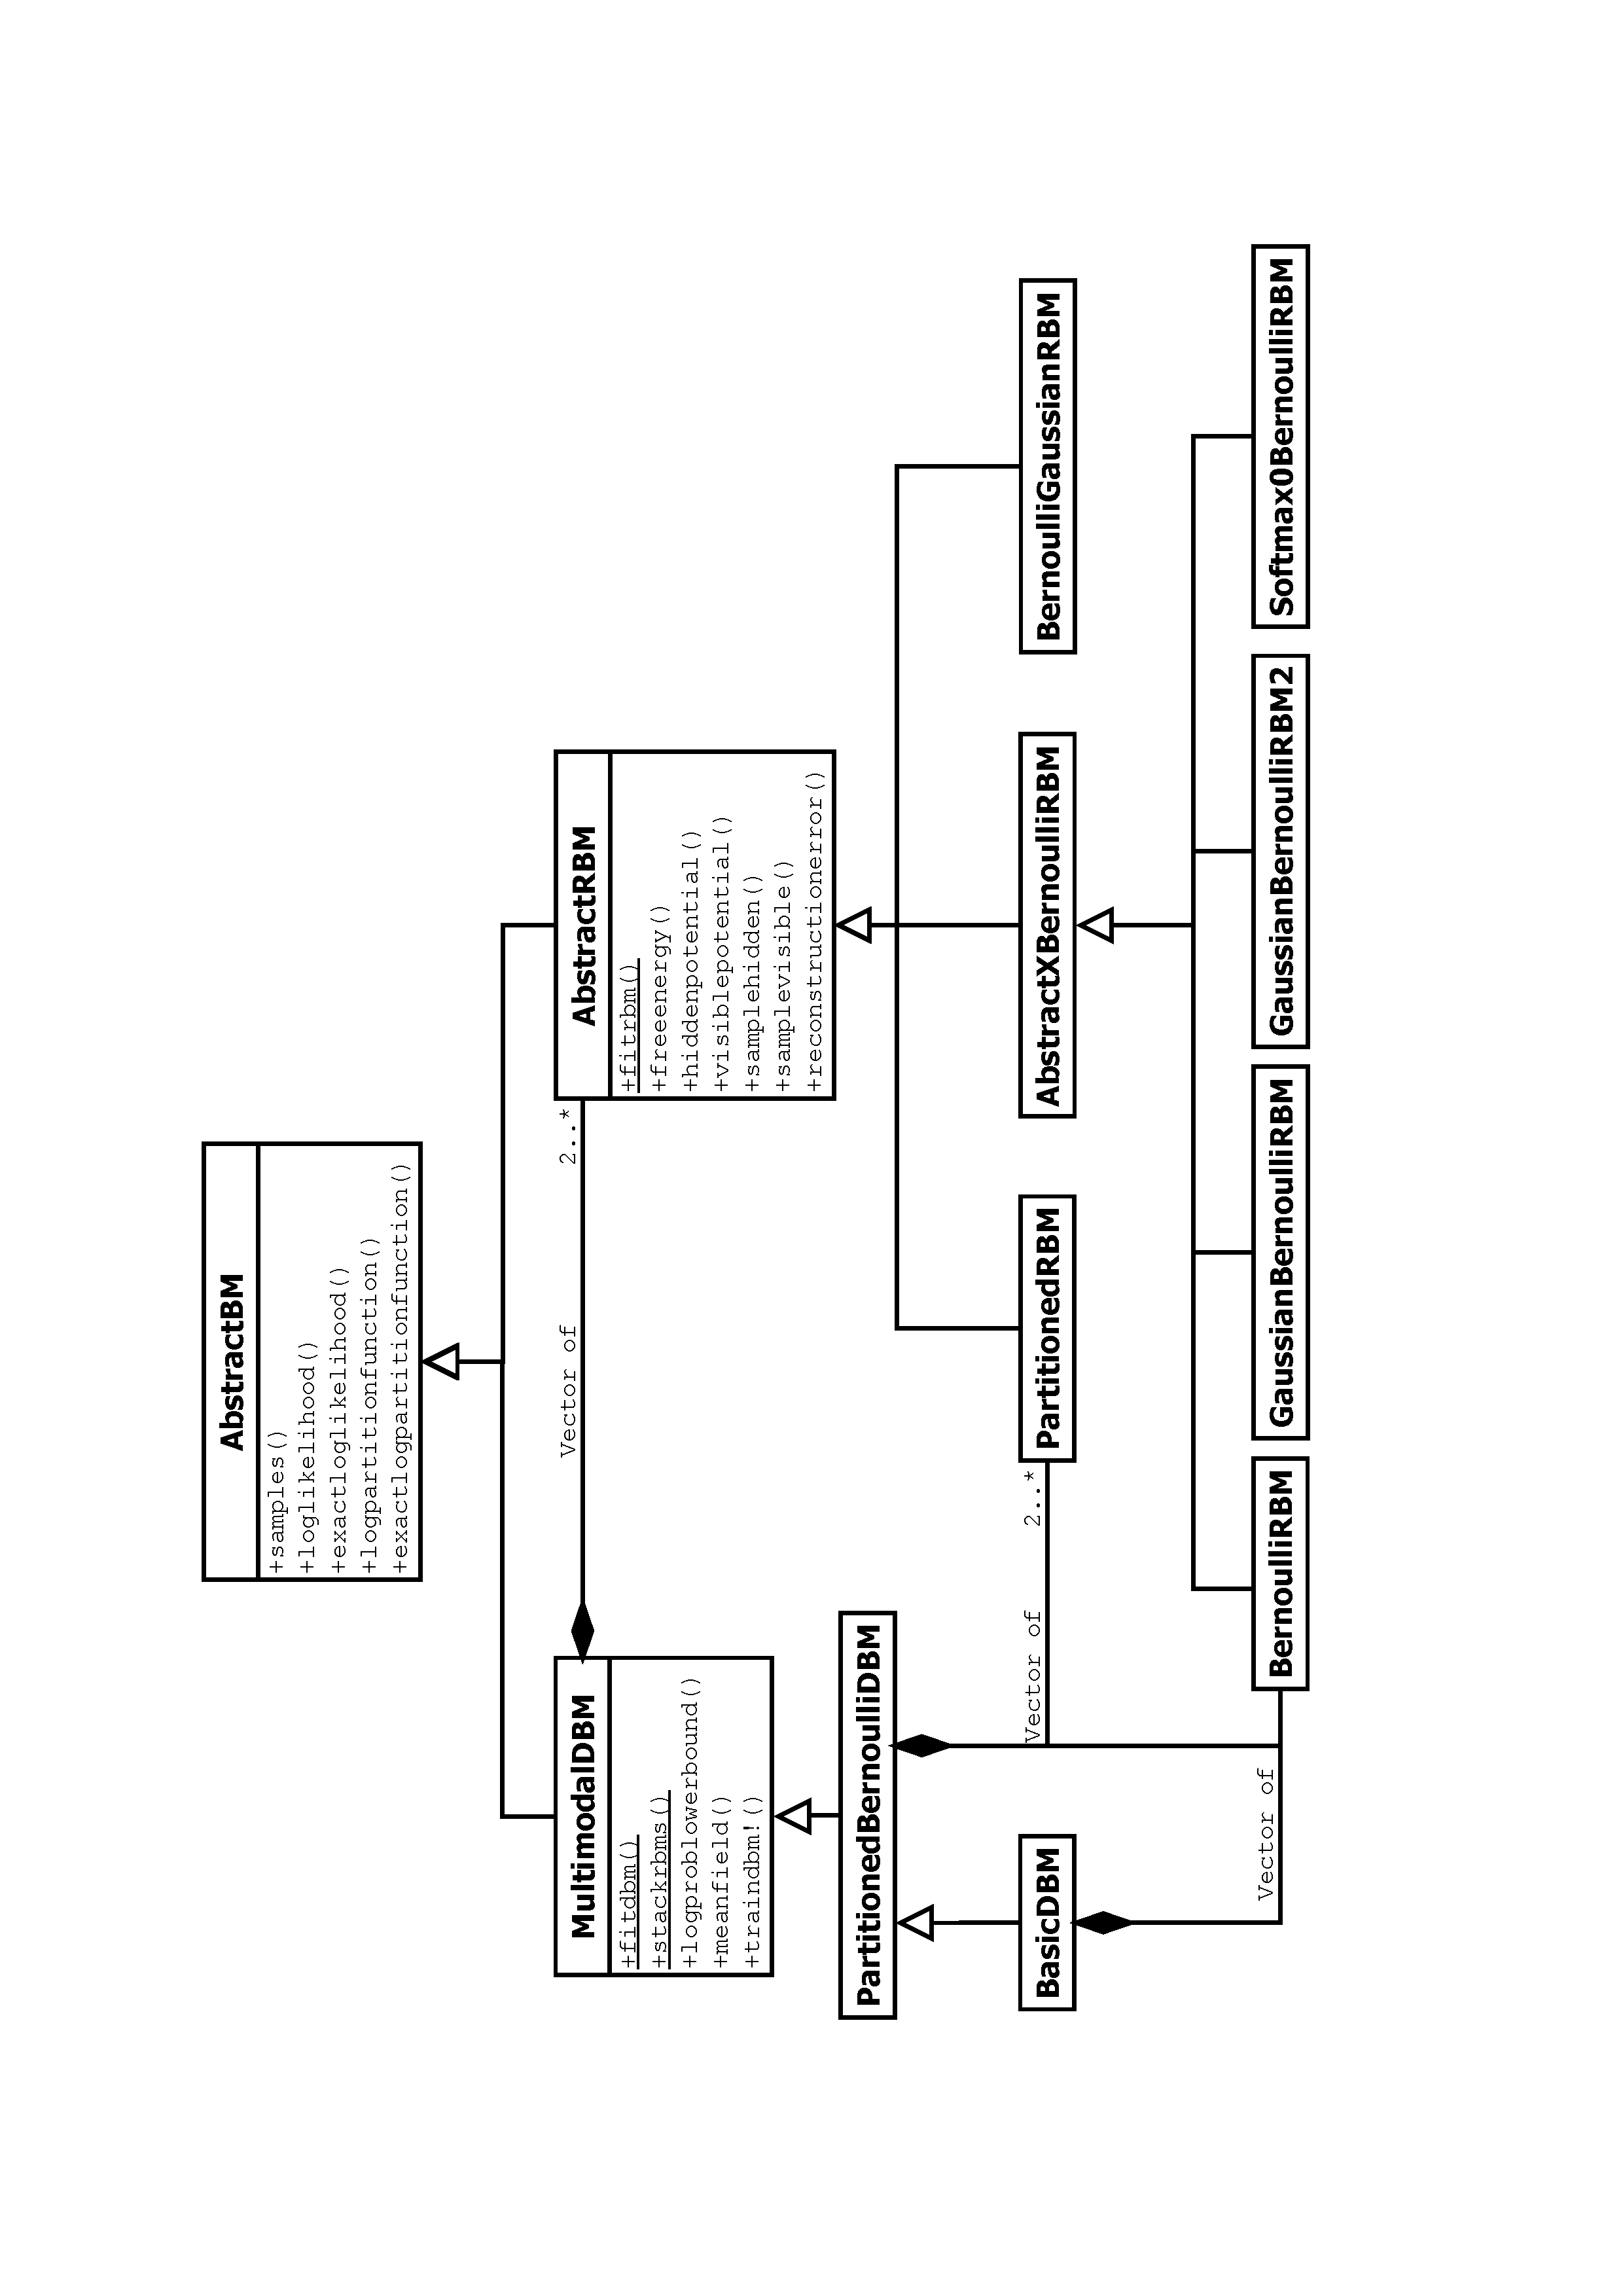
\includegraphics[scale=0.5,trim={5.2cm 4cm 6.8cm 3.4cm},clip,angle=-90]{images/BoltzmannMachinesDiagram.pdf}
   \caption{Overview of the type relationships together with the most important functions in the \apkg{Boltzmann machines} Julia package as a UML class diagram
%   For more details on these functions, see also tables \ref{juliaFunTableTrain} and \ref{juliaFunTableEval}.
   }
   \label{umlclassdiagram}
\end{figure}
\end{landscape}
}

All types of Boltzmann machines in the package have the common abstract supertype \inlinecode{AbstractBM}.
The functions that are available for all different subtypes can be seen in Figure \ref{umlclassdiagram} in the boxes below the type names.
For each of the models of Boltzmann machines, it is possible to generate samples by using Gibbs sampling via the \inlinecode{samples} function.
Conditional sampling is conveniently possible via this function (see \ref{usagesampling} and p.\ \pageref{bms_samples}).
Functions for evaluating the likelihood are also available for all implemented Boltzmann models.
For efficiently evaluating very small models, the likelihood and the partition function can be calculated exactly. This is also used for testing AIS by comparing the values estimated in small models to the exact ones.

The training is handled separately for DBMs and RBMs via the functions \inlinecode{fitdbm} and \inlinecode{fitrbm}, which can be used for fitting an RBM or DBM model, respectively.
These functions get as input a data set and all hyperparameters for training the model and return the model as output.
Table \ref{juliaFunTableTrain} gives an overview of all functions that can be used for training RBMs and DBMs.



\begin{table}[h]
\rowcolors{1}{gray!25}{white} % alternating row colors in tables
\caption{Functions in the Julia package for training RBMs and DBMs. All these functions return the trained model. The number of training epochs can be specified via the named argument \inlinecode{epochs}. There are many more hyperparameters which can be specified. For a more detailed description of the arguments, see the page references to the package documentation, which can be found in the appendix.}\label{juliaFunTableTrain}
\begin{tabularx}{\textwidth}{X}
 \Xhline{1pt}
   \inlinecode{fitrbm(x;...)} \rightpageref{bms_fitrbm} \\
   Fits a restricted Boltzmann machine model for a given data set \inlinecode{x} and additional model hyperparameters \\
   \inlinecode{stackrbms(x;...)} \rightpageref{bms_stackrbms}\\
   Pre-trains a stack of RBMs on a given data set \inlinecode{x}. It can either be used for pre-training of a DBM or to train a deep belief network. \\
   \inlinecode{traindbm!(dbm, x; ...)} \rightpageref{bms_traindbm!} \\
   Fine-tunes a DBM on the data set \inlinecode{x} using the mean-field approximation procedure \\
     \inlinecode{fitdbm(x; ...)} \rightpageref{bms_fitdbm} \\
   Fits a (multimodal) deep Boltzmann machine model for a given data set \inlinecode{x} and model hyperparameters \\
 \Xhline{1pt}
\end{tabularx}
\end{table}

Pre-training and fine-tuning of a DBM can either be done in one step via \inlinecode{fitdbm}, or in two separate steps.
Pre-training of DBMs or training of DBNs (see \ref{dbns}), can be performed via \inlinecode{stackrbms}.
DBMs  can be then be fine-tuned (see \ref{dbmtraining}) with the function \inlinecode{traindbm!}.
The fine-tuning algorithm is based on the mean-field approximation, which is calculated via the \inlinecode{meanfield} function.
The \inlinecode{traindbm!} function operates on a (pre-trained) DBM and modifies its weights.
The reason why the function name ends with an exclamation mark is that this is a Julia convention for functions that mutate their arguments.

The lower bound of the likelihood, which is the optimization objective of the DBM training algorithm, can be calculated via \inlinecode{logproblowerbound}.
This function is available for (multimodal) DBMs in addition to the ones listed for \code{AbstractBM}s.
An overview of the functions for evaluating the likelihood in RBMs and DBMs is given in Table \ref{juliaFunTableEval}.



\begin{table}[h]
\rowcolors{1}{gray!25}{white}
\caption{Functions in the Julia package for evaluating the likelihood of RBMs and DBMs. The partition function is estimated via AIS unless a value for the parameter \inlinecode{logz} is provided. The partition function cal can also be calculated exactly but this is only feasible for very small models. (For the algorithmic complexity of the corresponding algorithms, see \ref{methodExactloglik}.) }
\label{juliaFunTableEval}
   \begin{tabularx}{\textwidth}{X}
 \Xhline{1pt}
   \inlinecode{logpartitionfunction(bm; ... )} \rightpageref{bms_logpartitionfunction}\\
   Estimates log of the partition function of the Boltzmann machine \inlinecode{bm} using AIS. Additional hyperparameters for AIS may be provided. \\
   \makecell[tl]{
      \inlinecode{loglikelihood(rbm, x)} \\
      \inlinecode{loglikelihood(rbm, x, logz)}
   } \rightpageref{bms_loglikelihood} \\
   Calculates the log-likelihood of data \inlinecode{x} in the restricted Boltzmann machine model \inlinecode{rbm}. The log of the partition function can be provided as parameter \inlinecode{logz} or is estimated using AIS. \\
   \makecell[tl]{
      \inlinecode{loglikelihood(dbm, x; ...)} \\
      \inlinecode{loglikelihood(dbm, x, logz; ...)}
   } \rightpageref{bms_loglikelihood} \\
   Estimates the log-likelihood of a (multimodal) deep Boltzmann machine using AIS for each sample. Additional hyperparameters for AIS may be provided. \\
   \makecell[tl]{
   	\inlinecode{logproblowerbound(dbm, x; ...)} \\
   	   	\inlinecode{logproblowerbound(dbm, x, logz; ...)} \\
   	} \rightpageref{bms_logproblowerbound} \\
   Estimates the stochastic lower bound of the log-likelihood that is optimized by the training algorithm with mean-field optimization. \\
    \makecell[tl]{
    \inlinecode{aislogimpweights(rbm; ...)} \\
   \inlinecode{aislogimpweights(dbm; ...)}
   } \rightpageref{bms_aislogimpweights} \\
   Calculates (logarithmized) AIS importance weights for annealing from the given model to a null model as shown in \ref{figTwotypesais} A and B. Implicitly called by the functions above. \\
     \inlinecode{aislogimpweights(rbm1, rbm2; ...)}  \rightpageref{bms_aislogimpweights} \\
    Calculates AIS importance weights for annealing from one RBM model to another as shown in \ref{figTwotypesais} C.
    This can be used for comparing the likelihood of two RBM models directly.\\
       \inlinecode{exactloglikelihood(bm, x)} \rightpageref{bms_exactloglikelihood} \\
   Calculates the log-likelihood of a deep Boltzmann machine. \\
   \inlinecode{exactlogpartitionfunction(bm, x)} \rightpageref{bms_exactlogpartitionfunction} \\
   Calculates the log of the partition function for a restricted Boltzmann machine \\
 \Xhline{1pt}
\end{tabularx}
\end{table}


(Multimodal) DBMs are modeled as arrays (i.e.\ one-dimensional vectors) of RBMs.
In the UML diagram this composition of DBMs from vectors of RBMs is indicated by the UML composition relationship, which is depicted as line with filled diamond at the end.
Using RBMs as building blocks allows a very flexible composition of DBMs.
Figure \ref{mdbmimplasstack} shows how RBMs and \inlinecode{PartitionedRBM}s can be  arranged  and stacked to form \inlinecode{MultimodalDBM}s or \inlinecode{PartitionedBernoulliDBM}s.

An optimization of the algorithms for DBMs that contain only Bernoulli distributed nodes such as the \inlinecode{BasicDBM} or the \inlinecode{PartitionedBernoulliDBM} is possible by implementing specialized methods for these types.
For example, summing out nodes can be done more flexibly and effectively in DBMs with only Bernoulli distributed nodes (see Figure \ref{aissummingout}).

\begin{figure}[h]
   \centering
   
\includegraphics[scale=3.]{images/MDBMImpl.eps}
   \caption{Multimodal deep Boltzmann machines are modeled as a stack of restricted Boltzmann machines. On the left hand side, an example model is depicted as a graph and on the right hand side the corresponding modeling in the Julia package is shown.
   The first/lowest and the second layer are modeled as a \inlinecode{PartitionedRBM}s (white boxes with grey borders), each containing a vector holding two \inlinecode{BernoulliRBM}s (grey filled boxes).
   The third/highest layer is simply a \inlinecode{BernoulliRBM}.
   All three \inlinecode{AbstractRBMs} in a vector form the \inlinecode{MultimodalDBM}.
   The arrows indicate the ordering of the vectors.}
\label{mdbmimplasstack}
\end{figure}

Different types of RBMs are modeled as Julia composite types, which encapsulate the model parameters.
The abstract type for RBMs is \inlinecode{AbstractRBM}.
The methods listed there are implemented for all subtypes of RBMs in the package.
The function \inlinecode{samplehidden} and \inlinecode{samplevisible} are used for Gibbs sampling to sample from $p(h|v)$ and $p(v|h)$, respectively (see \ref{gibbssamplingrbm}).
The functions \inlinecode{hiddenpotential} and \inlinecode{visiblepotential} calculate the deterministic activation potential $\EX_v p(h|v)$ and $\EX_h p(v|h)$, which is used for RBM training and DBN training (see \ref{dbns}).
As recommended by \cite{hinton_practical_2012} the activation potential is used for the last update of the hidden units in Gibbs sampling (see Section 3.1 there), and the probabilities are also used for the visible states in the last step of sampling in the model distribution (Section 3.2 there).
Calculating the \inlinecode{visiblepotential} is also needed for sampling in DBNs as shown in Figure \ref{fig:dbn}, where the activation from the top layer is passed down to the visible layer in a deterministic way.
For each of these functions for sampling and calculating the activation potential, there is also a function that is suffixed with an exclamation mark.
These variants are mostly used in the implementation as they allow to reuse allocated space, which makes the implementation much faster.

The free energy of visible states $v$ in an RBM can be calculated via  \inlinecode{freeenergy(rbm, v)}.
This is used for calculating the likelihood, as described in equation (\ref{eqn:pRBMfreeenergy}) if a value for the partition function is given.
The free energy can also be used to compare the model fit of one RBM on different data sets, e.g., to monitor the overfitting by comparing the free energy in training and test data.
The \inlinecode{reconstructionerror} in RBMs (see \ref{reconstructionerror}) is also useful for monitoring, especially as a fast way to monitor the pre-training of DBMs.

The different RBMs described in \ref{rbmtypes} and \ref{methodsoftmax0} are implemented as subtypes of \inlinecode{AbstractXBernoulliRBM}.
This abstraction is useful for exploiting the commonalities between RBMs with Bernoulli distributed hidden nodes, and thereby reducing code duplication.

The \inlinecode{BernoulliGaussianRBM} is an RBM with Bernoulli distributed visible nodes and Gaussian hidden nodes.
This type was inspired by \cite{hinton_reducing_2006}, who use such an RBM layer with Gaussian hidden nodes in the top layer of a DBN for creating a better visualization of the dimensionality reduction.

The \inlinecode{PartitionedRBM} is used as a brace around RBMs in a layer such that a partitioned layer of RBMs can be thought of and used like any \inlinecode{AbstractRBM} in the implementations of other algorithms.



\subsubsection{Usage examples}\label{bmusage}
The \apkg{BoltzmannMachines} package has been registered in the official Julia package repository. It can be installed via the following Julia code:

\begin{lstlisting}[language=Julia]
import Pkg
Pkg.add("BoltzmannMachines")
\end{lstlisting}

The functions in the package expect the input as a matrix that contains the samples in the rows and the variables in the columns.
For the following examples, we assume that \inlinecode{x} is such a matrix of type \inlinecode{Array\{Float64,2\}} containing values of 0.0 and 1.0 with \inlinecode{nsamples} rows and \inlinecode{nvariables} columns.

\begin{lstlisting}[language=Julia]
nsamples, nvariables = size(x)
\end{lstlisting}

\paragraph{Training}\label{trainingimpl}

After loading the package via a \inlinecode{using} statement, training an RBM or a a DBM is as simple as calling \inlinecode{fitrbm} or \inlinecode{fitdbm}, respectively.

\begin{lstlisting}[language=Julia]
using BoltzmannMachines
rbm = fitrbm(x)
dbm = fitdbm(x)
\end{lstlisting}

But as hyperparameter tuning is very important, and the choice of the hyper parameters highly depends on the data set, using the default parameters will most likely not get an optimal result.
The most important hyperparameters for RBMs and DBMs are the number of hidden nodes, the number of epochs and the learning rate.

\begin{lstlisting}[language=Julia]
rbm = fitrbm(x; nhidden = 50, epochs = 200,
                learningrate = 0.001)
dbm = fitdbm(x; nhiddens = [50, 20], epochs = 200,
                learningrate = 0.001)
\end{lstlisting}

The learning rate and the number of epochs can also be specified for pre-training separately (see detailed description of the arguments of \inlinecode{fitdbm} on p.\ \pageref{bms_fitdbm}).
Furthermore, the hyperparameters for pre-training the RBM layers in a DBM can be specified individually for each layer.
For this purpose, the hyperparameters for each RBM can be defined in an array of designated objects of type \inlinecode{AbstractTrainLayer}.
Analogously to how RBMs are arranged as building blocks in DBMs (see Figure \ref{mdbmimplasstack}), these hyperparameter definition objects can be arranged in vectors and passed to \inlinecode{fitrbm} or \inlinecode{stackrbms}.
Objects of type \inlinecode{TrainLayer} are then translated to RBMs and objects of type \inlinecode{TrainPartitionedLayer} to partitioned RBMs.
For illustrating this, let us assume here that \inlinecode{x} has only 6 variables.
Then the code in Listing \ref{lst:partdbm} results in a model shown in Figure \ref{fig:smallpartitioneddbm}.
Each \inlinecode{TrainLayer} object is translated to train an RBM layer.
Via a call to \inlinecode{TrainPartitionedLayer}, the RBMs resulting from the contained \inlinecode{TrainLayer} objects are put next to each other on the same layer (see also Figure \ref{mdbmimplasstack}).

\begin{figure}[h]
   \centering
   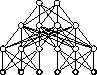
\includegraphics[scale=3.]{images/SmallPartitionedDBM.pdf}
   \caption{DBM architecture resulting from code in Listing \ref{lst:partdbm}}
\label{fig:smallpartitioneddbm}
\end{figure}

\begin{lstlisting}[language=Julia,caption={Fitting a partitioned DBM},label={lst:partdbm}, float=!h]
dbm = fitdbm(x; pretraining = [
      TrainPartitionedLayer([
         TrainLayer(nvisible = 3, nhidden = 3),
         TrainLayer(nhidden = 3)]),
      TrainLayer(nhidden = 4),
      TrainLayer(nhidden = 2)])
\end{lstlisting}

\FloatBarrier
\paragraph{Customizing the optimization}

The calculation of the gradients is abstracted from Gibbs sampling and mean-field approximation.
The default is the optimization via the gradients described in \ref{rbmtraining} and \ref{dbmtraining}, which are calculated from the input of the contrastive divergence, Gibbs sampling and mean-field algorithms.
The gradients calculated from this input can be customized, e.g., for adding a regularization term, by creating a new subtype of \inlinecode{AbstractOptimizer} (see p.\ \pageref{bms_AbstractOptimizer}) and passing it to the training function or specifying it in a \inlinecode{TrainLayer} object via the \inlinecode{optimizer} argument.


\paragraph{Different types of visible nodes}

For training RBMs or DBMs types with other types of visible nodes, such as those for data with variables that have more than two categories, the type of the RBM can be specified as argument \inlinecode{rbmtype} for \inlinecode{fitrbm} function or in the \inlinecode{TrainLayer} object for training an RBM.
Additional parameters, such as the specification of the number of categories for each categorical variable, can also be defined there.

Let us assume that \inlinecode{xcat} contains eight categorical variables with values of 0.0 and 1.0 in the first four variables and values 0.0, 1.0, and 2.0 in the second four variables.
The encoding in dummy variables as described in \ref{methodsoftmax0} can then be done with the \inlinecode{oneornone\_encode} function (see p.\ \pageref{bms_oneornone_encode}).
The resulting binary matrix can then be used as input to the training function.
The following code exemplifies this by training a DBM with two hidden layers on the categorical data in \inlinecode{xcat}:

\begin{lstlisting}[language=Julia]
categories = [fill(2, 4); fill(3, 4)];
x01 = oneornone_encode(xcat, categories)
dbm = fitdbm(x01;
      pretraining = [
         TrainLayer(nhidden = 7, categories = categories,
               rbmtype = Softmax0BernoulliRBM);
         TrainLayer(nhidden = 6)
      ])
\end{lstlisting}

\paragraph{Generating synthetic data}\label{usagesampling}
Synthetic data can be generated with the \inlinecode{samples} function, which expects the Boltzmann machine model and the number of samples as arguments.
The function works for RBMs as well as for DBMs.

\begin{lstlisting}[language=Julia]
ngensamples = 500
samples(dbm, ngensamples)
\end{lstlisting}

Sampling is performed with the Gibbs sampling algorithm.
For each of the generated samples, randomly initialized, independent Gibbs chains are run.
A hyperparameter for Gibbs sampling is the number of burn-in steps, which can be specified via the \inlinecode{burnin} parameter (see p.\ \pageref{bms_samples}).

Conditional sampling, here e.g., with the first and third variable being set 1.0, and the second variable set to 0.0, can be also be done with this function:

\begin{lstlisting}[language=Julia]
samples(dbm, 500; conditions = [1 => 1.0; 2 => 0.0; 3 => 1.0])
\end{lstlisting}

For re-using allocated space, there is also the functions \inlinecode{gibbssample!} for running Gibbs sampling on pre-allocated matrices of samples, and, analogously, there is \inlinecode{gibbssamplecond!} for conditional sampling (see p.\ \pageref{bms_gibbssample!}).

\paragraph{Evaluating and monitoring}\label{monitoring}

Monitoring is the evaluation of a model during the training time.
This can be used for hyperparameter tuning.
If the resulting learning curve \citep{ml_encyclopedia} \dots
\begin{itemize}
\item \dots is unstable or not going in the right direction, the learning rate needs to be reduced.
\item \dots is smooth but too flat, the learning rate can be increased.
\item \dots has not reached a plateau/valley at the end of training, the number of epochs can be increased.
\item \dots is getting better on the training data set but not on a test data set, overfitting is happening.
\end{itemize}

Evaluating a model is usually done using also other data sets than the training data set to detect overfitting.
The function \inlinecode{splitdata} (see p. \pageref{bms_splitdata}), can be used to conveniently split the data set into, e.g., a training and a test data set.
Here we use 80\%  of the original data set \inlinecode{x} as training data and 20\% as test data.

\begin{lstlisting}[language=Julia]
xtrain, xtest = splitdata(x, 0.2)
\end{lstlisting}

Monitoring the training progress can be done via passing monitoring functions and data for monitoring data as arguments to the training functions.

The advantage of this approach is that is very simple to pass any kind of user defined function, e.g., for printing information about the training progress.
\begin{lstlisting}[language=Julia]
fitrbm(x; epochs = 20,
       monitoring = (rbm, epoch) -> println(epoch))
\end{lstlisting}

The \inlinecode{fitdbm} function allows to monitor the pre-training as well as the fine-tuning.
An overview of the most important pre-defined functions that can be used for monitoring can be found in Table \ref{monfun}.
For each of the training functions in Table \ref{juliaFunTableTrain}, there is also a function prefixed with ``\inlinecode{monitoring\_}", which allows to write the monitoring with functions in Table \ref{monfun} in a compact way.
This works also for other user-defined functions that accept the same input arguments as the pre-defined monitoring functions.

\begin{lstlisting}[language=Julia,caption={Monitoring pre-training and fine-tuning}, label={lst:monfitdbm}]
datadict = DataDict("Training data" => xtrain,
                        "Test data" => xtest);
monitors, dbm = monitored_fitdbm(x; nhiddens = [6,2],
      epochs = 20, learningrate = 0.05,
      monitoringpretraining = monitorreconstructionerror!,
      monitoring = monitorlogproblowerbound!,
      monitoringdata = datadict);
\end{lstlisting}

In Listing \ref{lst:monfitdbm}, the different data sets that are to be used in monitoring are at first collected in a \inlinecode{DataDict} object and then passed to the training function via the  \inlinecode{monitoringdata} argument.
For monitoring the pre-training of higher layers, the input data in the \inlinecode{datadict} is propagated upwards by using the induced deterministic activation potential in the same way as it is done with the data for training the higher layers.

The monitoring functions are expected to write their results in the \inlinecode{Monitor} objects (see p.\ \pageref{bms_Monitor}) that are received as first argument of the monitoring functions.
These \inlinecode{Monitor} objects are collected and returned in form of a vector as the first result of the monitored training function.



\begin{table}[h]
\rowcolors{1}{gray!25}{white}
\caption{Monitoring functions in the \apkg{BoltzmannMachines} Julia package}
\label{monfun}
   \begin{tabularx}{\textwidth}{X}
 \Xhline{1pt}
   \inlinecode{monitorreconstructionerror!(monitor, rbm, epoch, datadict)} \rightpageref{bms_monitorreconstructionerror!}\\
     Monitors the reconstruction error in an RBM \\
     \inlinecode{monitorfreeenergy!(monitor, rbm, epoch, datadict)} \rightpageref{bms_monitorfreeenergy!}\\
Monitors the free energy in an RBM \\
     \inlinecode{monitorloglikelihood!(monitor, rbm, epoch, datadict; ...)} \rightpageref{bms_monitorloglikelihood!}\\
Monitors the (estimated) log-likelihood in an RBM \\
        \inlinecode{monitorexactloglikelihood!(monitor, bm, epoch, datadict)} \rightpageref{bms_monitorexactloglikelihood!}\\
Monitors the exact log-likelihood in an RBM or DBM \\
     \inlinecode{monitorlogproblowerbound!(monitor, dbm, epoch, datadict; ...)} \rightpageref{bms_monitorlogproblowerbound!}\\
  Monitors the (estimated) variational lower bound of the log likelihood in a DBM \\
   \Xhline{1pt}
\end{tabularx}
\end{table}

The collected values can be plotted via the accompanying plotting package \apkg{Boltzmann\-Machines\-Plots}, which is also registered in the Julia package repository.
The plotting functionality has been separated in a separate package because plotting is not available in the base installation of Julia.
By making the dependency to a plotting package optional, plotting functionality must only be installed if it is needed.
The plotting is performed with \apkg{Gadfly} \citep{gadfly}, one of the Julia plotting packages with the most stable stable API, which has already reached version 1.0.
\apkg{BoltzmannMachinesPlots} can be installed and imported in the same way as the main package:

\begin{lstlisting}[language=Julia]
import Pkg
Pkg.add("BoltzmannMachinesPlots")
using BoltzmannMachinesPlots
\end{lstlisting}

The \inlinecode{plotevaluation} function, which is defined there, takes care of plotting the information of a \inlinecode{Monitor} object.
For examples of such monitoring plots, see Figure \ref{fig:monitoring_bmplots}.
\begin{lstlisting}[language=Julia]
plotevaluation(monitors[1]) # pre-training of first RBM layer
plotevaluation(monitors[3]) # fine-tuning
\end{lstlisting}


\begin{figure}[h]
   \centering
   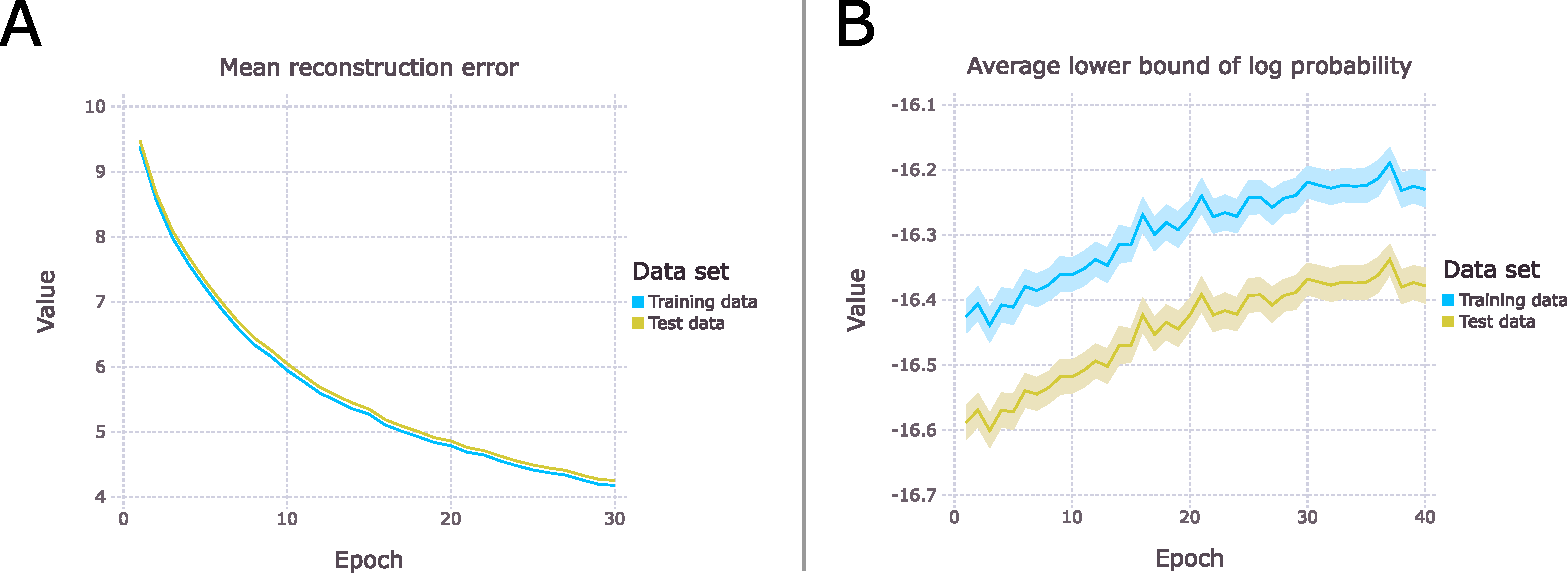
\includegraphics[scale=.59]{images/bmplots_curves.pdf}
   \caption{Two examples for monitoring plots created with the \apkg{BoltzmannMachinesPlots} package}
\label{fig:monitoring_bmplots}
\end{figure}


\paragraph{Dimension reduction}

In addition to their capabilities as generative models, DBMs can also be used for dimension reduction.
The hidden layers of a DBM correspond to an increased abstraction of the input data,
with nodes in higher layers encoding more abstract patterns than the nodes in the layers below.
Intuitively, this dimension reduction can be thought of as looking at the ideas that the network has about its input.
If in the top hidden layer only two nodes are used for encoding the information, the activation patterns resulting from the input can be visualized as point in the 2D plane.
For this, each input sample is used to induce activation in the network, resulting in one 2D point that is defined by the activation of the nodes in the top layer.
The \inlinecode{scatterhidden} function of \apkg{BoltzmannMachinesPlots} package does this in a convenient way.
It creates a scatter plot of the logit-transformed mean-field activation in the top hidden layer of a DBM, given the input data and the DBM.



\FloatBarrier
\clearpage
\section{Connecting R and Julia with the \apkg{JuliaConnectoR}}\label{juliaconnectorpart}

R is a very popular language in bioinformatics and biostatistics \citep{bioconductor}.
Making algorithms written in Julia also available in R enlarges the group of possible users, particularly in the field of life sciences.
To access functionality from other programming languages, a language bridge is needed.
In this particular case, the language bridge was needed to integrate the functionality of the \apkg{BoltzmannMachines} package into the DataSHIELD infrastructure for distributed privacy-preserving analyses \citep{gaye_datashield}, which is based on R.
For this purpose, a new approach was chosen, resulting in the creation of the \apkg{JuliaConnectoR} R package, which has been published in the Comprehensive R Archive Network.\footnote{\url{https://cran.r-project.org/package=JuliaConnectoR}}

There are two other R packages for calling Julia from R, namely \apkg{JuliaCall} \citep{JuliaCallPaper} and \apkg{XRJulia} \citep{chambersExtendingR}, which predate the \apkg{JuliaConnectoR}.
The main reason for developing a new software was that the other packages did not work reliably.
One issue was run-time stability, which is important for a software that needs to be deployed across a number of different sites and that has to function without human intervention.
Of course, also during local development, crashes are not desirable.
Other issues were the incompatibilities with some R and Julia versions and a lack of documentation.
The fresh start allowed to design a clean interface and to develop several new and unique features.

\subsection{Feature overview and comparison to existing solutions}
A user-friendly design was the most important concern when developing the \apkg{JuliaConnectoR}.
This includes ease of use, a clearly defined interface, and stability.
Table \ref{tab:JuliaConnectoRFeatures} lists the most relevant features.
For a comparison, the packages \apkg{JuliaCall} and \apkg{XRJulia} are also regarded in the table.

\begin{table}[h!]
\centering
\caption{\label{tab:JuliaConnectoRFeatures} Comparison of features between the
\apkg{JuliaConnectoR} (version 0.6), \apkg{JuliaCall} (version 0.17.1) and
\apkg{XRJulia} (version 0.9.0).}
\begin{tabular}{p{6.75cm} p{1.9cm} p{2.05cm} p{2cm} p{1.2cm}}
\hline \\ [2ex]\\
 & \begin{rotate}{25}\apkg{JuliaConnectoR} \end{rotate} &
 \begin{rotate}{25} \apkg{JuliaCall} \end{rotate} &
 \begin{rotate}{25} \apkg{XRJulia} \end{rotate} &
 See \\
\hline 
\\\\[-4\medskipamount]
Communication & TCP/binary & \proglang{C} interface & TCP/JSON &
\ref{juliaconnectorCommuncation} \\
Automatic importing of packages & Yes & No & No &
\ref{juliaconnectoRAutoimport} \\
Specification for type translation & Yes & No & No &
\ref{translatejuliar} \\
Reversible translation from Julia to R & Yes
& No & No & \ref{translatejuliar} \\
\proglang{R} data frames to \proglang{Julia} Tables & Yes & Yes & No &
\ref{juliaconnectordataframes} \\
Missing values & Yes & Yes & No & \ref{juliaconnectorMissings} \\
Callbacks & Yes & Yes & No & \ref{juliaconnectorcallbacks} \\
Interruptible & Yes & No & (Yes) & \ref{juliaconnectorinterrupting} \\
Show standard (error) output & Yes & No & Yes &
\ref{juliaconnectorOutput} \\
Let-syntax & Yes & No & No & \ref{juliaconnectorDbmexample} \\
\\[-2\medskipamount]
\hline
\end{tabular}
\end{table}

In the following, these features and the differences between the packages are detailed.
Subsequently, in \ref{juliaconnectorDbmexample}, it is demonstrated how these features help to train and evaluate DBMs in R.
In appendix \ref{JuliaConnectoRDoku}, the documentation of the \apkg{JuliaConnectoR} package can be found.
There, the usage of the different functions is described in greater detail from a user perspective.

\subsubsection{Communication protocol}\label{juliaconnectorCommuncation}

The \apkg{JuliaConnectoR} communicates with Julia via the transmission control protocol (TCP) \citep{tcpspec}.
TCP is also used by Julia for multi-processing and distributed computing.
Also other R machine learning packages, e.g., \apkg{h2o} \citep{h2o} and \apkg{sparklyr} \citep{sparklyr}, communicate via TCP with their back-ends, which perform the actual computations.
The \apkg{JuliaConnectoR} uses a custom binary format to transfer content between Julia and R.
The format is inspired by BSON \citep{bsonspec}, which is a binary alternative to the text-based JavaScript Object Notation \citep{jsonspec1}.
The main advantage of this custom format is that it can utilize the binary form of vectors and matrices in R and Julia.
This allows to use the \inlinecode{writeBin} and \inlinecode{readBin} functions in R for directly writing complete objects into the output stream or reading them from the input stream, respectively.
Analogously, in Julia the functions \inlinecode{write} and \inlinecode{read} can be used to write and read objects in binary form.
As the binary representations of numeric vectors and matrices are largely the same, these parallels between Julia and R can be exploited to minimize the communication overhead.
An additional measure for reducing the communication overhead is to stream the messages, which allows to start reading content in Julia while R is still writing, and vice versa.

\apkg{JuliaCall} builds on the Julia package \apkg{RCall} \citep{rcallGithub} to bridge Julia and R.
\apkg{RCall} and \apkg{JuliaCall} use the C-interfaces of R and Julia to exchange data between the processes.
On the one hand, this tighter connection brings speed advantages compared to TCP.
On the other hand, such a low-level integration is much harder to maintain and develop.
This was reflected by the fact that \apkg{JuliaCall} did not work reliably when I started to working on the \apkg{JuliaConnectoR}.
Also when testing the functionality for the comparison here, using \apkg{JuliaCall} led to crashes of the R session on multiple occasions.
With the high frequency of new Julia releases, the costs of maintaining a low-level interface increase substantially.
Keeping complexity low is particularly important for creating sustainable open source software \citep{midha_improving_2010}.
This aspect was kept in mind in the design of the \apkg{JuliaConnectoR}.
As a result, the higher-level approach taken by the \apkg{JuliaConnectoR} is compatible with a wide range of R and Julia versions (R 3.2-4.0 and Julia 1.0-1.6), requiring only minimal adaptions for keeping cross-version compatibility.
Another disadvantage of the coupling via a C-interface is that this requires that R is built shared/dynamic library.
For using \apkg{RCall}, this is required\footnote{The option \inlinecode{-enable-R-shlib} is required when installing R, see installation instructions of \apkg{RCall}: \url{https://github.com/JuliaInterop/RCall.jl/blob/v0.13.4/docs/src/installation.md}}.
When installing R, R is not configured by default as shared/dynamic library because this can reduce the performance of R by 10-20\% \citep{rAdmin}.


\apkg{XRJulia} uses also TCP as underlying communication mechanism but it transports the information via JSON messages.
These messages can also contain vectors, matrices and complex nested objects.
As JSON is text-based, numeric values have to be transformed to from their binary form into decimal values and their textual representation to be wrapped in a JSON message.
This additional overhead slows down the communication, in particular for larger matrices and vectors.
Therefore, \apkg{XRJulia} escapes the strategy of using TCP for these cases.
Instead, large arrays are written to temporary binary files on the hard drive (see \inlinecode{largeVectors} documentation item in the manual of \apkg{XRJulia}).
Yet, writing files to the hard disk involves additional costs compared to using TCP directly.
Communication via local files also prevents using Julia as a server and R as a client on different machines.
Although the mechanism for setting such a remote connection is not exposed in the \apkg{JuliaConnectoR}, the potential for this is there.
Security considerations are the main reason why this is not fully supported in the \apkg{JuliaConnectoR}.
There is the possibility for securing TCP connections via Secure Shell (SSH) tunnels \citep{ylonen_ssh}.
After an integration SSH tunneling with the \apkg{JuliaConnectoR}, such a mechanism could allow to run Julia remotely and work locally in R.
This may be used to employ remote servers that provide compute power but do not offer the same convenience as a local machine, e.g., if a integrated development environment such as RStudio \citep{rstudio} cannot be used on a remote server.

%Another usage scenario for remote TCP connections is when using container technology.
%Wrapping software and the resources into containers can aid in creating software for reproducible research \citep{docker_reproducible}.
%The communication between containers is also done via TCP.
%A container that bundles Julia code and its dependencies together with a \apkg{JuliaConnectoR} communication component could be used to wrap functionality for R in a similar way as it is done for 

\subsubsection{Automatic importing of packages and modules}\label{juliaconnectoRAutoimport}

One of the main reasons for using a language bridge such as the \apkg{JuliaConnectoR} is to access functionality from packages in other languages while being able to do most of the work in a language that is more familiar or more suitable for the rest of the task.
An example for this can be to use deep learning in Julia but perform data preprocessing and plotting in R.

The function \inlinecode{juliaImport} (see also on p.~\pageref{rdokitem_juliaImport}ff.) of the \apkg{JuliaConnectoR} can inspect a Julia package and then return all Julia functions, including type constructors, in the form of an environment that contains R functions that wrap the Julia functions.
This approach helps to handle foreign packages in a simple way, and it aids in writing more concise code, as can be seen in the following.

At first, a minimal example, employing the \apkg{Flux} Julia package in R, is shown in Listing \ref{fluximportJulia} and Listing \ref{fluximportR}.
Later, in Section \ref{juliaconnectorDbmexample}, a more detailed example using DBMs and the \apkg{BoltzmannMachines} package is given.
This should demonstrate that the \apkg{JuliaConnectoR} can be used for importing arbitrary packages.
In Listing \ref{fluximportJulia} and Listing \ref{fluximportR}, two different packages are involved.
The first package that is imported into R is the Julia package \inlinecode{Pkg}.
This package is contained in the Julia standard library.
Its purpose is to install and manage other packages.
In this example, \inlinecode{Pkg} is used to install the \apkg{Flux} package in version 0.11.
Then, \apkg{Flux} is used to define a feed-forward neural network, which has two hidden layers, and which uses a rectified linear activation function in the first hidden layer.


\begin{lstlisting}[language=Julia,float=!h,caption={Julia code for importing the \apkg{Flux} package and defining a small neural network},label={fluximportJulia}]
import Pkg
Pkg.add(name = "Flux", version = "0.11")
import Flux
model = Flux.Chain(Flux.Dense(4, 4, Flux.relu), 
                   Flux.Dense(4, 1))
\end{lstlisting}

Using the \inlinecode{juliaImport} function of the \apkg{JuliaConnectoR}, the R code shown in Listing \ref{fluximportR} can do the same as the Julia code in Listing \ref{fluximportJulia}.

\begin{lstlisting}[language=R,numbers=left,float=!h,caption={R code using the \apkg{JuliaConnectoR} for  doing the same as in Listing \ref{fluximportJulia}},label={fluximportR}]
library(JuliaConnectoR)
Pkg <- juliaImport("Pkg")
Pkg$add(name = "Flux", version = "0.11")
Flux <- juliaImport("Flux")
model <- Flux$Chain(Flux$Dense(4L, 4L, Flux$relu),
                    Flux$Dense(4L, 1L))
\end{lstlisting}

An alternative to importing a package in this way is to address the functions via their name as strings via the \inlinecode{juliaCall} function. 
For example, the lines 2 and 3 in Listing \ref{fluximportR} could be replaced with:
\begin{lstlisting}[language=R]
juliaEval("import Pkg")
juliaCall("Pkg.add", name = "Flux", version = "0.11") 
\end{lstlisting}
(For more information on \inlinecode{juliaEval}, which simply evaluates a given string in Julia and returns the result, see p.~\pageref{rdokitem_juliaEval}. 
For more details on the usage of \inlinecode{juliaCall} see p.~\pageref{rdokitem_juliaCall}.)

When considering the next lines, the advantage of the automatic importing becomes more obvious.
Replacing the imported functions with \inlinecode{juliaCall} there would deteriorate the legibility in a significant way.
In case of the \inlinecode{relu} function, it is not possible to replace it with \inlinecode{juliaCall}, as the function is not called but only referenced.
The activation function is specified via passing a function as an argument, which is here the \inlinecode{relu} function.
In the R code in Listing \ref{fluximportR}, this becomes also possible because the \inlinecode{relu} function has been imported as a function object and the \apkg{JuliaConnectoR} recognizes imported functions and can translate them back to Julia functions.
Passing functions as arguments to other functions is typical for a functionally oriented style.
Enabling functional programming was an important consideration in the design of the \apkg{JuliaConnectoR}.

An additional nice side benefit of using \inlinecode{juliaImport} is that the auto-complete functionality in the R terminal or in RStudio can aid in typing and finding functions that are collected in the returned environment.

When developing Julia code, writing functions inside a module, which is defined in one or more files, is a good practice because it allows to easily replace the complete code in the Julia session with a single call of the \inlinecode{include} function in Julia.
Moreover, using module files makes debugging easier because errors can be tracked more easily when the line number in the file is specified in the error output.
It is also possible to import such local Julia modules into R via \inlinecode{juliaImport} in a similar way as shown above with Julia packages.
For examples, see the documentation of \inlinecode{juliaImport} (p.~\pageref{rdokitem_juliaImport}ff.).

\subsubsection{Translation between Julia and R}\label{translatejuliar}
Notable in Listing \ref{fluximportR} is that the numbers needed to be passed as integers (e.g., ``\inlinecode{4L}'' instead of simply ``4'').
The \inlinecode{Dense} function of the \apkg{Flux} package is sensitive to the types of its input arguments and it is necessary here that the arguments are of type \inlinecode{Int} in Julia.
If, e.g. floating point numbers of type \inlinecode{Float64} are passed, the \inlinecode{Dense} function would yield a different result.
This is because the multiple dispatch mechanism in Julia determines which specific method is chosen, dependent on the types of the input arguments.
Using the exact type is not important in all cases because it is also possible to handle types in Julia in a more relaxed way, e.g., by specifying abstract types or not specifying types for arguments in the definition of functions.
Examples for such abstract types are \inlinecode{Number}, or the type \inlinecode{Any}, which is most unspecific.
It is also not possible to infer the type automatically, because it is possible that the results of different methods, which are invoked for different argument types, are completely different.
Therefore, a \apkg{JuliaConnectoR} user must care about the types of the arguments exactly if the user also would need to care about them when using the functions directly in Julia.

Given that types are important in Julia, the translations of the types are clearly documented for the \apkg{JuliaConnectoR} (see p.~\pageref{juliaconnectordokutypetranslation}).
Although the translation of the basic types is largely the same in \apkg{JuliaCall} and \apkg{XRJulia}, these packages lack a formal specification of the translations.
The attempt to translate complex values (e.g., via \inlinecode{juliaCall("typeof", 1i)}) resulted in an error in \apkg{XRJulia}.

Another distinctive feature of the the \apkg{JuliaConnectoR} is that it ensures that the translations from Julia to R are fully reversible.
Single values, vectors and matrices of primitive types in Julia are translated directly to vectors and matrices in R.
If a Julia vector or matrix can be mapped to a vector or matrix in R but its type cannot be matched exactly, the information about the original Julia type is attached to the translated object in R.
If such a translated object is passed to Julia again, it can be reconstructed with its original type.
For example, if a Julia package operates with single-precision floating point values and a function returns an object of type \inlinecode{Vector\{Float32\}}, this vector can be translated to an R \inlinecode{double} vector with double-precision floating point values, and the information about the original type is added as an attribute in R.
If this vector is passed to Julia later, it is implicitly converted to the original type.

For efficiency purposes, the \apkg{JuliaConnectoR} does not translate composite objects by default.
Instead, they are passed to R in form of proxy objects, which hold references to the original objects and can be used in their place.
With the \inlinecode{juliaGet} function (see p.~\pageref{rdokitem_juliaGet}), also composite objects can be fully translated to R objects in form of nested R lists.
From these lists, which are annotated with information about the original Julia types, the original objects can be reconstructed later.
This way, the objects can be serialized in R and saved with the R session, unless, of course, an object contains external references such as file handles or pointers to allocated memory.

\apkg{XRJulia} and \apkg{JuliaCall} also work with proxy objects for types that are more complex than arrays of primitive types.
\apkg{JuliaCall} cannot translate such objects to R data structures.
\apkg{XRJulia} also has a \inlinecode{juliaGet} function, which can translate objects from Julia to R.
A full reconstruction of such objects in Julia is not possible, however, since the type information is not managed.


\paragraph{Data frames}\label{juliaconnectordataframes}

Data in tabular form is very common in data science. Most biomedical data sets consist of one or more tables.
Therefore, it is important to deal with this kind of data in an interface between two languages that are used by data scientists.

In R, data of tabular structure is kept in objects of the class \inlinecode{data.frame}.
There are also additional packages such as \apkg{tibble} \citep{tibble} and \apkg{data.table} \citep{datatable} providing tabular data structures which are compatible with the R \inlinecode{data.frame} interface.
In Julia, tabular structures are not part of the standard library but they are only available in separate packages.
In addition defining a data type for holding tabular structure, the Julia package \apkg{DataFrames} \citep{juliaDataFramesGithub} offers tools for working with tabular data.
Its design is inspired by the R package \apkg{dplyr} \citep{dplyr} and the Python package \apkg{pandas} \citep{pandas}, which aim to streamline data analysis by offering solutions for many common data analysis tasks.
There are also other packages supporting tabular structures that do not build on the \apkg{DataFrames} package.
To unify the different approaches, the \apkg{Tables} package was created, which defines an minimal common interface.
This interface is used by the \apkg{DataFrames} package and also by many other packages, e.g., by the \apkg{CSV} \citep{juliacsvGithub} package for reading CSV files and the \apkg{JuliaDB} package \citep{juliadbGithub} for working with large persistent data sets.
Due to the broader goal of the \apkg{DataFrames} Julia package, it has reached version 1.0 only very recently (April 21st 2021) and there have been many breaking changes in the course of the development.
Because the interface of the \apkg{Tables} has been stable for a longer time, with version 1.0 released in February 2020, and because of its lightweight implementation, the \apkg{Tables} package was used as the basis for the support of tabular structures in the \apkg{JuliaConnectoR}.
The minimal interface of the \apkg{Tables} interface also allows to use the translated data structures in Julia without applying additional transformations, which would be required to create a \inlinecode{DataFrames.DataFrame}.

\apkg{JuliaCall} depends on the \apkg{DataFrames} package and translates R data frames to Julia objects of type \inlinecode{DataFrames.DataFrame}.
\apkg{XRJulia} translates R data frames to Julia objects of type \inlinecode{Dict\{String, Any\}}.
This is not compatible to the \apkg{Tables} interface, which regards only dictionaries with keys of type {Symbol} as tables.
Moreover, the order of the columns is lost by the translation to a dictionary.

\apkg{JuliaCall} translates Julia data frames directly to R \inlinecode{data.frame} objects.\footnote{For example, \inlinecode{julia\_call("identity", iris)} returns again an R data frame.}
The \apkg{JuliaConnectoR} does not translate structures satisfying the Julia \apkg{Tables} interface by default.
Firstly, it is better to avoid translating large amounts of data if it not necessary.
It is also not possible to convert all Julia objects that are classified as Julia \apkg{Tables} to R data frames.
For example, the \apkg{Tables} package regards all dictionaries with keys of type \inlinecode{Symbol} as tables.
For example, the dictionary \inlinecode{Dict(:x => [[1,2],"a"])} is considered to be a table by \apkg{Tables} (version 1.3.1).
Yet, this data structure cannot be converted to an R data frame.
Therefore, the translation to R data frames must be requested explicitly.
This can be done with the function \inlinecode{as.data.frame}, which is specialized for Julia proxy objects (see p.~\pageref{rdokitem_as.data.frame.JuliaProxy}).


\paragraph{Missing values}\label{juliaconnectorMissings}

Missing values are common in biomedical data. Both R and Julia support missing values.
The two languages deal with them in a slightly different way, which needs to be respected when translating between R and Julia.

R allows missing values directly in vectors of numeric and character values.
For this, R designates certain values to encode the value of \inlinecode{NA}.
In R double vectors, values of \inlinecode{NaN} and \inlinecode{NA} are distinguished.
The value of \inlinecode{NaN}, which indicates that the value is ``not a number'', is defined in the international standard concerning floating point values \citep{floatingpointstandard}.
R extends this standard and uses one of the several representations of \inlinecode{NaN} as the \inlinecode{NA} value in R.
This makes it possible that both \inlinecode{c(1,NA)} and \inlinecode{c(1, NaN)} are of type \inlinecode{double}.

Julia has also a concept for missing values.
In contrast to R, missing values are represented by the \inlinecode{missing} object, which is of type \inlinecode{Missing}. Accordingly, the vector \inlinecode{[1.0, missing]} is of type \inlinecode{Array\{Union\{Missing, Float64\},1\}}, while \inlinecode{[1.0, NaN]} is of type \inlinecode{Array\{Float64,1\}}.

The \apkg{JuliaConnectoR} makes sure that \inlinecode{NA} values in R are translated to \inlinecode{missing} values in Julia and vice versa, while \inlinecode{NaN} values are treated as floating point values according to the standard.
In the following code snippet, this is demonstrated via performing an addition of two R vectors in Julia:

\begin{lstlisting}
R> juliaCall("+", c(1, NA, NaN), c(1, 2, 3))
[1] 2 NA NaN
\end{lstlisting}


In \apkg{JuliaCall}, calling \inlinecode{julia\_call("identity", NA)} for translating a value of \inlinecode{NA} to Julia and back to R produced a fatal error, terminating the R session.
In \apkg{XRJulia} the call \inlinecode{juliaCall("identity", NA)} returns \inlinecode{NULL} and gives a warning message.
For both packages there is no definition of how these values shall be handled between R and Julia.


\paragraph{Callbacks: Translating R functions to Julia functions}\label{juliaconnectorcallbacks}

As mentioned before in \ref{juliaconnectoRAutoimport}, the \apkg{JuliaConnectoR} can translate a Julia function to an R function that invokes the Julia function.
R functions created in that way can be translated directly back to the original Julia functions.
Listing \ref{juliafunascallback} shows an example for this.
At first, a Julia function is defined in Julia with \inlinecode{juliaEval}.
The returned value, which is the newly defined function, can be assigned to an R variable, which contains the wrapped Julia function (line 1).
The Julia function \inlinecode{map} applies a given function on a vector of values.
It is used here as a simple example of a function that receives another function as an argument.
In line 2 it is used for applying the \inlinecode{times2} function in Julia.
The return value is finally also translated to R (line 3). 

\begin{lstlisting}[language=R, float =!h, caption={Passing a reference to a Julia function back to Julia},label={juliafunascallback}, numbers=left]
R> times2 <- juliaEval("times2(x) = 2*x")
R> juliaCall("map", times2, c(1,2,3))
[1] 2 4 6
\end{lstlisting}

In contrast to R functions that wrap Julia functions, normal R functions are translated as {\em callback} functions.
That means, they are translated to Julia functions that invoke the original R functions.
Listing \ref{rfunascallback} shows how an R function can be passed to Julia and used as a callback function.

\begin{lstlisting}[language=R, float =!h, caption={An R function used as a callback function}, label={rfunascallback}]
R> times2 <- function(x) {2*x}
R> juliaCall("map", times2, c(1,2,3))
[1] 2 4 6
\end{lstlisting}

The code in Listing \ref{rfunascallback} is less efficient than the code in Listing \ref{juliafunascallback}, because in Listing \ref{rfunascallback}, Julia and R need to communicate in every separate application of the \inlinecode{times2} function.
However, this mechanism makes it possible to interweave R and Julia code.
In such a simple case, this is, of course, not really beneficial.
In \ref{juliaconnectorDbmexample}, a more useful example for using callback functions is given.
It shows how an R function can be used for displaying monitoring output during the training of a deep learning model.
In such a scenario, the overhead of calling back to R after every training epoch is negligible when compared to the overall computation time.

Passing R functions to Julia is also possible with \apkg{JuliaCall}.
\apkg{XRJulia} does not have that feature. 
With the lower communication overhead via the C interface, \apkg{JuliaCall} has a speed advantage compared to the \apkg{JuliaConnectoR} when there is a high number of calls between R and Julia.
However, in a deep learning scenario, where usually long-running functions are used, this is less important.
There, stability and ways to get feedback from long-running tasks become more important.

\subsubsection{Features for interactive use}

When developing new code or experimenting with existing solutions, it is essential to gain insights into the behavior of the software and to be able to influence it easily.
This includes the possibility to interrupt a running program or inspecting intermediate output.
Accordingly, the \apkg{JuliaConnectoR} supports these features.

\paragraph{Interrupting}\label{juliaconnectorinterrupting}

Some training hyperparameters have a strong influence on the execution times of deep learning algorithms.
When experimenting with different hyperparameters, it can be desired to stop the execution of a function call if the remaining time seems too long.
When working with the \apkg{JuliaConnectoR}, this becomes viable.
Calls to Julia via \apkg{JuliaConnectoR} can be interrupted in the same way as R function calls.
When using \apkg{XRJulia}, interrupting calls to Julia is also possible.
This is not very stable, however, and it can happen that it is needed to restart the R session because the connection to Julia cannot be established anymore.
Attempting to interrupt a call to Julia via \apkg{JuliaCall} does not work or results or in a crash of the R session.

This behavior can be tested, e.g., by executing \inlinecode{juliaEval('while true; end')} for the \apkg{JuliaConnectoR} and \apkg{XRJulia}, or \inlinecode{julia\_eval('while true; end')} for \apkg{JuliaCall}.

\paragraph{Output redirection}\label{juliaconnectorOutput}

Long-running tasks often produce output on the command line to give the user feedback about the progress.
For example, downloading and installing a package with all its dependencies may take some time.
In both R and Julia, the package management prints output on the command line to inform the user about the success of failure of the different installation steps.
In deep learning, getting feedback about the training progress is desirable for estimating the time that is needed for training a model.
While feedback may also be given via callback functions, this approach only works if the software offers this option.
Moreover, when developing own algorithms, printing information and having access to warning messages is essential for debugging a program.
Therefore, the redirection of standard output and standard error output is an important feature for a language bridge that is used in an interactive way.

The \apkg{JuliaConnectoR} displays the standard output and the standard error output from Julia on the R command line.
The Julia output is redirected to R in an asynchronous way.
This allows that the output is displayed before the function returns, which is important for the reporting of progress.
\apkg{XRJulia} can also do this. Standard output or standard error output is not visible when using \apkg{JuliaCall}.



\subsection{Using \apkg{BoltzmannMachines} in R via the \apkg{JuliaConnector}}\label{juliaconnectorDbmexample}
The previous examples for using the \apkg{JuliaConnectoR} were kept minimal to demonstrate the basic features of the package in a compact way.
The next examples show how easy it becomes to translate Julia code to R code that calls Julia behind the scenes.
For this purpose some examples from using the \apkg{BoltzmannMachines} package, shown in \ref{bmusage}, are translated to R.
Additionally, these examples shows how DBMs can be trained in R via the \apkg{BoltzmannMachines} package.
As mentioned in \ref{BMfeatures}, there is currently no R package that implements deep Boltzmann machines.
But via the \apkg{JuliaConnectoR}, all features of the \apkg{BoltzmannMachines} package become conveniently usable in R.

It is assumed in the following that the variable \inlinecode{x} is a double matrix in R that contains values of 0.0 and 1.0.
The rows of \inlinecode{x} contain the different samples and the columns the values for different variables.

At first, the \apkg{BoltzmannMachines} package needs to be installed in Julia and imported into R in the same way as demonstrated with the \apkg{Flux} package in Listing \ref{fluximportR} (p.~\pageref{fluximportR}):

\begin{lstlisting}[language=R, float=!h]
library(JuliaConnectoR)
Pkg <- juliaImport("Pkg")
Pkg$add("BoltzmannMachines")
BMs <- juliaImport("BoltzmannMachines")
\end{lstlisting}

After this, all functions in the \apkg{BoltzmannMachines} package are available via the variable \inlinecode{BMs} and fitting DBMs and RBMs is possible.

\begin{lstlisting}[language=R, float=!h]
rbm = BMs$fitrbm(x)
dbm = BMs$fitdbm(x)
\end{lstlisting}
 
Partitioned architectures can also be built via specifying the arguments for the different parts via \inlinecode{TrainLayer} objects.
Translating the code in Listing \ref{lst:partdbm} (p.~\pageref{lst:partdbm}) to R results in the following code:

\begin{lstlisting}[language=R,caption={Fitting a partitioned DBM in R via the \apkg{JuliaConnectoR}},label={lst:partdbmr}, float=!h]
dbm <- BMs$fitdbm(x, pretraining = list(
          BMs$TrainPartitionedLayer(list(
             BMs$TrainLayer(nvisible = 3L, nhidden = 3L),
             BMs$TrainLayer(nhidden = 3L))),
          BMs$TrainLayer(nhidden = 4L),
          BMs$TrainLayer(nhidden = 2L)))
\end{lstlisting}

The functions of the \apkg{BoltzmannMachines} package are strict concerning the argument types and it is required that the numbers have the correct types.
For passing a vector of complex objects to Julia, such as the vector of objects in the \inlinecode{pretraining} argument, R lists can be used.
These are translated to vectors with the most specific type that can be inferred from the arguments.
In this case, the inferred type of the vector is \inlinecode{Array\{AbstractTrainLayer,1\}} as the common supertype of \inlinecode{TrainLayer} and \inlinecode{TrainPartitionedLayer} is \inlinecode{AbstractTrainLayer}.

To use monitoring during DBM training, the easiest way is to use the \inlinecode{monitored\_fitdbm} function (see p.~\pageref{bms_monitored_fitdbm}).
The usage of this function has previously been exemplified in Listing \ref{lst:monfitdbm} (p.~\pageref{lst:monfitdbm}).
The translation to R can be found in Listing \ref{lst:monfitdbmr}.

\begin{lstlisting}[language=R,caption={Monitoring pre-training and fine-tuning}, label={lst:monfitdbmr}, float = !h, numbers=left,style=rlststyle]
xtrain_xtest <- BMs$splitdata(x, 0.1)
xtrain <- xtrain_xtest[[1]]
xtest <- xtrain_xtest[[2]]
datadict <- juliaLet('BoltzmannMachines.DataDict(
                        "Training data" => xtrain,
                        "Test data" => xtest)',
                     xtrain = xtrain, xtest = xtest)
monitors_dbm <- BMs$monitored_fitdbm(x, nhiddens = c(6L,2L),
      epochs = 20L, learningrate = 0.05,
      monitoringpretraining = BMs$@\backtick@monitorreconstructionerror!@\backtick@,
      monitoring = BMs$@\backtick@monitorlogproblowerbound!@\backtick@,
      monitoringdata = datadict)
monitors <- monitors_dbm[[1]]
dbm <- monitors_dbm[[2]]
\end{lstlisting}

For monitoring the data is split into training and test data before the training (lines 1-3 in Listing \ref{lst:monfitdbmr}).
In contrast to Julia, R cannot assign two variables in one statement.
To have two different variables for training and test data, the return value of \inlinecode{BMs\$splitdata}, which is a proxy object for a \inlinecode{Tuple} of Julia objects, has to be disjoined.
This can be done by indexing the proxy object (lines 2-3).
(For more information on indexing proxy objects, see p.~\pageref{rdokitem_AccessMutate.JuliaProxy}ff.)

Then the \inlinecode{DataDict} can be created (lines 4-7 in Listing \ref{lst:monfitdbmr}), which will be passed to the monitoring functions.
The straightforward way to create a dictionary in Julia uses syntax that is not available in R.
A convenient way to construct objects involving complex Julia syntax via the \apkg{JuliaConnectoR} is to use the \inlinecode{juliaLet} function (see p.~\pageref{rdokitem_juliaLet}ff.).

After this preparation of the data that is used for monitoring, the training is performed via calling \inlinecode{monitored\_fitdbm} in lines 8-12 in Listing \ref{lst:monfitdbmr}.
The monitoring functions of the \apkg{BoltzmannMachines} package can be passed as arguments via R.
The names of these functions end with exclamation marks, as it is the convention for Julia functions that mutate their arguments.
For the use in R, the function names need to be enclosed with backticks (lines 10-11).

The \apkg{JuliaConnectoR} allows to fully translate Julia objects into R objects.
This can be used to translate a DBM to an R object and serialize it with the R session.
It can also be used to bring the monitoring information in R for plotting it there.
The \apkg{BoltzmannMachinesRPlots} package\footnote{\url{https://github.com/stefan-m-lenz/BoltzmannMachinesRPlots}} can create plots from monitoring information that is available in R.

\begin{lstlisting}[language=R, float = !h]
library(BoltzmannMachinesRPlots)
plotMonitoring(juliaGet(monitors))
\end{lstlisting}

The plotting functionality is based on the \apkg{ggplot2} package \citep{ggplot2}  and the \apkg{gridExtra} package \citep{gridExtra} for displaying all information conveniently in one plot.
The resulting plots are similar to ones shown in Figure \ref{fig:monitoring_bmplots} (p.~\pageref{fig:monitoring_bmplots}).

It is also possible to produce plots already during the training by utilizing R callback functions (see also \ref{juliaconnectorcallbacks}).
A simple example for this is shown in Listing \ref{callbackexample}.
The corresponding plot is shown in Figure \ref{fig:callbackplot}.

The function \inlinecode{plotValVsEpoch} (lines 8-18 in Listing \ref{callbackexample}) creates a new plot evaluates the model and adds the result of the evaluation to the plot in subsequent epochs.
This can, e.g., be passed to \inlinecode{fitrbm} as \inlinecode{monitoring} argument (line 21). (For the arguments of \inlinecode{fitrbm}, see p.~\pageref{bms_fitrbm}).
Callback functions can also be used for monitoring DBMs via the \inlinecode{monitoring} argument of \inlinecode{TrainLayer} (see p.~\pageref{bms_TrainLayer}) or the \inlinecode{monitoring} argument of \inlinecode{fitdbm} (see p.~\pageref{bms_fitdbm}).

The evaluation used here is the euclidean distance between the covariance matrix of synthetic samples, which are generated by the RBM or DBM model, and the covariance matrix of the original data (lines 1-4 in Listing \ref{callbackexample}).
The implementation of \inlinecode{covDistSamples} is not very efficient because it calls again back to Julia to generate the samples and then calculates the distance in R.
However, this shows the flexibility of customizing the monitoring.
The example in Listing \ref{callbackexample} also demonstrates the possibility of getting live feedback about the training, which is particularly relevant when the training takes a long time.

\noindent\begin{minipage}{\linewidth}
\captionsetup{type=listing}
\begin{lstlisting}[language=R, caption={Using an R function as a callback function during RBM training}, label={callbackexample}, numbers = left]
covx <- cov(x)
covDistSamples <- function(bm) {
   norm(cov(BMs$samples(bm, 2000L)) - covx, type = "2")
}

epochs <- 70L

plotValVsEpoch <- function(bm, epoch) {
   val <- covDistSamples(bm)
   if (epoch == 1) {
      ymax <- max(val)
      plot(x = 1, y = val,
           xlim = c(0, epochs), ylim = c(0, ymax*1.1),
           xlab = "Epoch", ylab = "Value")
   } else {
      points(x = epoch, y = val)
   }
}

rbm <- BMs$fitrbm(x, epochs = epochs, learningrate = 0.01,
                  monitoring = plotValVsEpoch)
\end{lstlisting}

\captionsetup{type=figure}
   \centering
   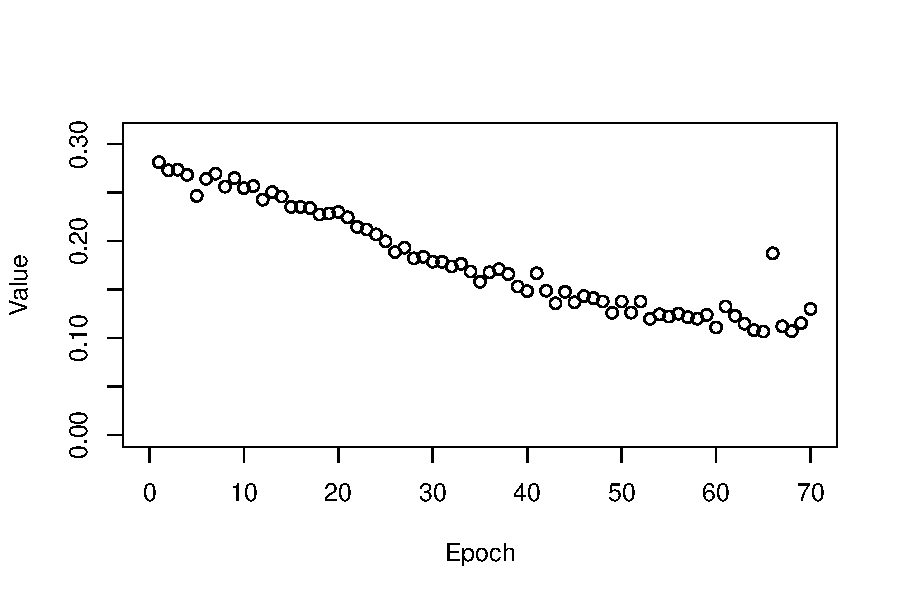
\includegraphics[scale=.95,trim={0cm 0.5cm 0cm 0cm}]{images/callbackplot.pdf}
   \caption{Exemplary plot created via the code in Listing \ref{callbackexample}}
\label{fig:callbackplot}
\end{minipage}
\clearpage




%\subsection{Implementation details}
%\begin{table}
%\begin{tabular}{lcl}
%\hiderowcolors
%message & = & '0x01' call \\
	 & $\mid$ &'0x00' element \\
	 & $\mid$ &'0x50' output \\
	 & $\mid$ &'0x5e' output \\
	 & $\mid$ &'0xff' fail \\
	 & $\mid$ &byebye \\
call & = & string list \\
list & = & int32 \{element\} int32 \{named\_element\} attributes \\
attributes & = & nattributes \{named\_element\} \\
nattributes & = & uint8 \\
named\_element & = & string element \\
element & = & '0x00' \\
		& $\mid$ &'0x01' dimensions \{double\} attributes \\
		& $\mid$ &'0x02' dimensions \{complex\} attributes \\
		& $\mid$ &'0x03' dimensions \{raw\} attributes \\
		& $\mid$ &'0x04' dimensions \{integer\} attributes \\
		& $\mid$ &'0x05' dimensions \{boolean\} \\
		& $\mid$ &'0x06' dimensions \{string\} attributes \\
		& $\mid$ &'0x07' list \\
		& $\mid$ &'0x5b' string (* name of symbol *) \\
		& $\mid$ &'0x5e' object\_class\_id object\_reference \\
		& $\mid$ &'0xcb' callback \\
		& $\mid$ &'0xee' expression \\
		& $\mid$ &'0xfc' named\_function \\
object\_class\_id & = & '0x5c' (* class JuliaStructProxy *) \\
				& $\mid$ &'0x5a' (* class JuliaSimpleArrayProxy *) \\
				& $\mid$ &'0xaf' (* anonymous function reference *) \\
				& $\mid$ &'0xaa' (* class JuliaArrayProxy *) \\
				& $\mid$ &'0x00' (* no information *) \\
object\_reference & = & 8 * byte \\
anonymous\_function\_reference & = & 8 * byte \\
callback & = & string \\
named\_function & = & string \\
string & = & int32 utf8string \\
dimensions & = & ndimensions \{int32\} \\
ndimensions & = & int32 \\
output & = & int32 \{byte\} \\
fail & = & string \\
byebye & = & '0xbb' \\
%\end{tabular}
%\caption{Serialization grammar for the \apkg{JuliaConnectoR}. TODO: Tabelle aufteilen und erklären}
%\end{table}
%
%EBNF syntax \citep{ebnf} für die Grammatik erklären

%* A string is preceded by the number of bytes to UTF-8-encode the string.
%* The sequence of unnamed/positional elements in a list is preceded by
%  the number of (named) elements that follow.
%* Standard output (after '0x50') or standard error output (after '0x5e')
%  is preceded by the number of bytes that are sent.


\clearpage
\FloatBarrier
\section{Deep generative models in DataSHIELD}\label{deepgends}

If data of individuals is distributed across different clinics/sites and data protection constraints prevent that the data leave the sites, a joint analysis is not possible in a simple way. 
A practical approach to this problem is taken by DataSHIELD \citep{budin-ljosne_datashield}, a software framework for privacy-preserving analyses of distributed biomedical data, which allows conducting several important types of statistical analyses on distributed data.
The implementations of the algorithms are based on reformulating the underlying algorithms in a way that only aggregated data has to leave the sites.
However, not all algorithms are suitable to be applied in such a way.
For example, it is possible to train deep learning models on distributed data by transferring the models between the sites during the training.
This approach can yield results without much  performance loss but it requires that the model parameters are exchanged between the sites very often \citep{chang_distributed}.
Since the number of model parameters in neural networks may even exceed the amount of training data, and there are many small training steps that need to be performed, this approach leads to an extensive data flow between the sites.
This in turn raises practical issues because the networks need to be serialized, transferred, and deserialized, which can consume much time for large networks.
But most importantly, it makes it hard to argue that no individual data leave the sites if large quantities of data are exchanged.
An alternative approach to conduct analyses in such a scenario is to use synthetic data \citep{bonofiglio2020}.
The goal of synthetic data is to create data that captures the underlying structure of the original data but is not linked to the individuals and can be used without or with less privacy restrictions compared to the original data.
In this chapter I first investigate the feasibility of distributed analyses based on synthetic observations generated from deep generative approaches.
This includes a comparison of DBMs with two other neural network approaches, GANs and VAEs, and with multiple imputation as a simpler method.
Finally, I introduce a software based on the DataSHIELD infrastructure that can generate synthetic data using DBMs.

\subsection{Theoretical background}

\subsubsection{Privacy concepts}\label{privacyconcepts}
If synthetic data are generated from real patient data, it is particularly important to evaluate not only the usability of the synthetic data for conducting analyses but also to assess the risk of leaking private information that may result from releasing the synthetic data.
There is always a trade-off between privacy and usability \citep{dinur_revealing_2003, kifer_no_2011}.
This means, absolute guarantees of privacy are impossible in all practical cases.
If the model learns information from data, there is always some information about the original data points contained.
This opens the door for probabilistic reasoning about the original data.
For example, if a data point is left out from the training data, this will influence the output of a meaningful learning algorithm.
Even the estimation of a mean value can be influenced strongly by an outlier, which may be used to infer some probability whether such an outlier was used to estimate the mean.
The goal is therefore not to exclude disclosure entirely but to minimize it while permitting meaningful analyses.

Given a data set generated by a model that has been trained on a training data set, the concept of {\em membership privacy} \citep{li_membership_2013} focuses on describing the risk of whether an attacker can guess if a point is in the training set.
A privacy breach is defined as a positive membership disclosure, i.e., that an attacker can assert with a high probability that an individual data point is included in the training data \citep{li_membership_2013}.

$\varepsilon$-differential privacy is a particular approach for achieving membership privacy \citep{dwork_differential_2008}.
Intuitively, it requires that the output of an algorithm is not affected too much by single data points in the training data set \citep{li_membership_2013}.
The pre-specified parameter $\varepsilon$ defines a boundary on how much influence is allowed by a single data point.
For models that are trained via gradient descent optimization, such as most neural networks, there is a way to satisfy $\varepsilon$-differential privacy by addding noise and clipping the gradients during training \citep{abadi_deep_2016}.
This, of course, will decrease the quality of the model.

A simpler approach for membership privacy is {\em $k$-anonymity} \citep{sweeney_k_anonymity_2012}.
It requires some attributes in a data set to be defined as ``quasi-identifiers", to which an attacker may have access for identifying an individual.
The requirement for a $k$-anonymous data set is then that all released data contains more than $k$ individuals for each combination of quasi-identifiers.
For $k > 1$, there will then always be more than one record found by querying identifying attributes.
An attacker can therefore not be certain that a record belongs to a certain individual.
This does not exclude, however, that an attacker may still gain useful information about individuals, e.g., if the records having the same combination of quasi-identifiers are very similar in the other attributes or if an attacker has additional knowledge.
Some weaknesses of $k$-anonymity are targeted by proposed refinements, which introduce additional parameters for indicating the privacy level \citep{machanavajjhala_l-diversity_2007, li_t-closeness:_2007}.

Common to all these approaches is that they define a level of privacy that is determined by one or more parameters.
These parameters cannot really be calculated and are somewhat subjective. All these approaches for achieving privacy do not provide absolute certainty and merely serve as tools to minimize the disclosure risk.

Moving on from theoretical privacy concepts, we take a look at a practical implementation for conducting privacy-preserving analyses next.

\subsubsection{The DataSHIELD framework}

DataSHIELD ({\em D}ata {\em A}ggregation {\em T}hrough
{\em A}nonymous {\em S}ummary-statistics from {\em H}armonised {\em I}ndividual
lev{\em EL} {\em D}atabases) \citep{budin-ljosne_datashield} is open source software for the privacy-preserving analysis of individual-level data that may be distributed across different sites.
Most of the algorithms implemented in DataSHIELD rely on communicating aggregated statistics instead of individual data.
These are considered to be sufficiently non-disclosive to be shared across sites.
The basic principle of the software is shown in Figure \ref{fig:datashieldprinciple}.

 \begin{figure}[h]
   \centering
   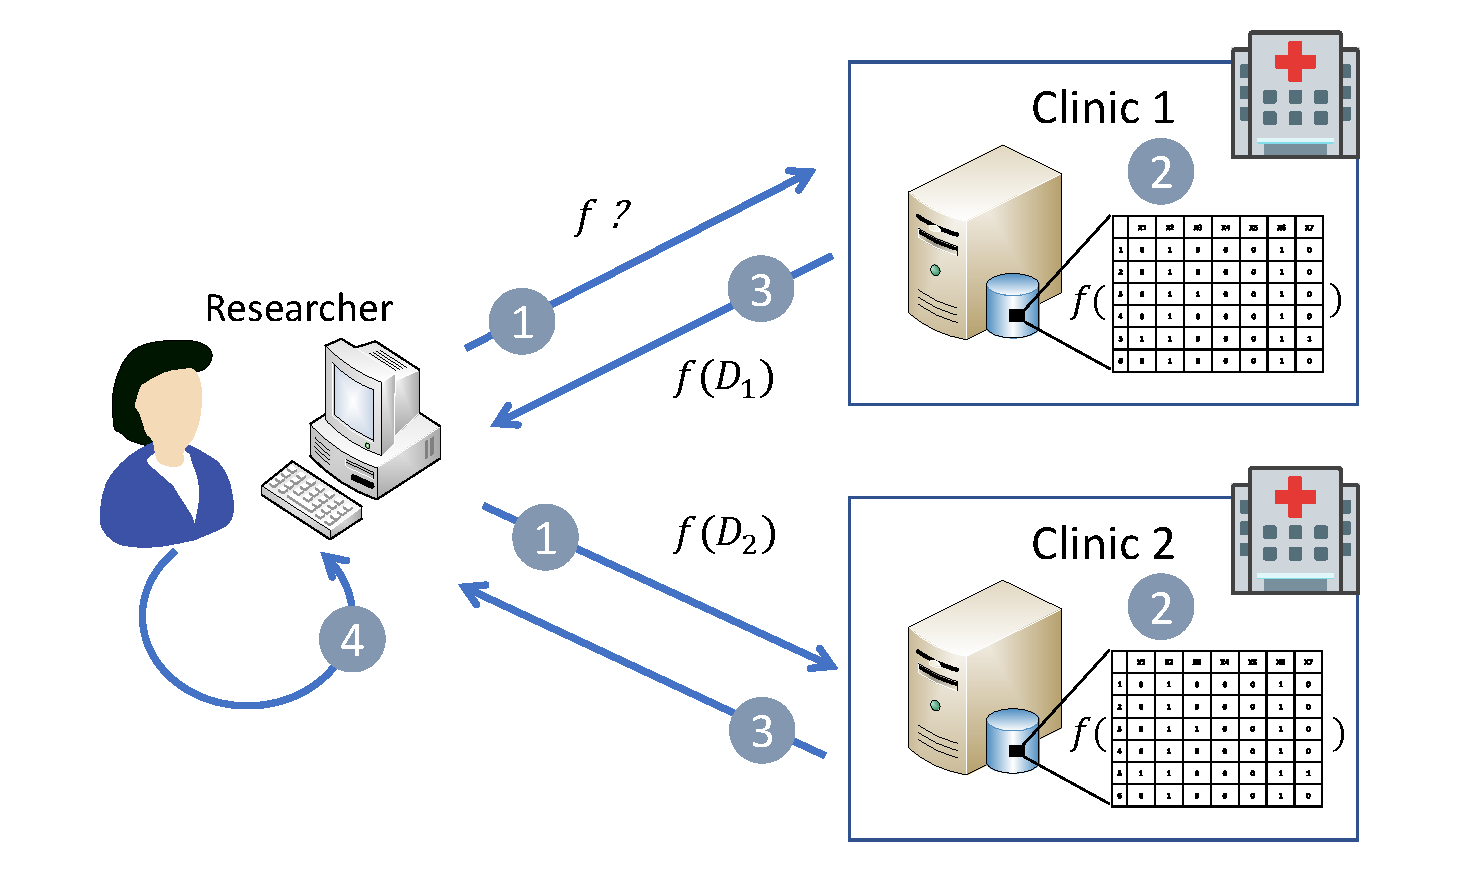
\includegraphics[scale=0.6]{images/datashieldprinciple.pdf}
   \caption{The principle of DataSHIELD. For calculating a desired statistic in a cohort that is distributed across multiple data centers, the DataSHIELD analysis client sends requests \circlenum{1} to the participating sites for the researcher. \circlenum{2} On each site runs an analysis server that manages the data and controls the access. If the requests are allowed, the analysis routine is executed on the data. \circlenum{3} The return values are aggregated statistics, which can be transferred to the user without breaching data protection. \circlenum{4} On the analysis client, the aggregated statistics are combined to calculate the desired statistic.}
   \label{fig:datashieldprinciple}
 \end{figure}

Pre-requisite for performing analyses with DataSHIELD is that the data at the different sites must be harmonized and that the necessary client-server infrastructure must be set up properly.

The client software is provided as the \apkg{dsBaseClient} R package, which is available from GitHub\footnote{https://github.com/datashield/dsBaseClient}.
In principle, the client software can be installed and used on any computer running R.
In practice, however, it makes sense to provide an analysis client on a central RStudio server.
Researchers who want to conduct analyses can get access to this server and find a computation environment that is ready to use.
This has the additional advantage that the firewalls of the analysis servers can be configured to accept only requests from the IP of the central analysis server, which adds an extra layer of security \citep{gruendner}.

The servers of the DataSHIELD infrastructure that run at the different sites and hold the data are called {\em Opal} servers \citep{opal}.
The Opal servers manage the data and control the access to it.
The data is stored in tabular form and the rights to view or analyze data can be set on the level of tables.
All R functions that are allowed to be executed locally must be registered in the Opal server.
An incoming request is only executed if the function that is called via the request is in the set of allowed functions and if the user is authorized to access the data in Opal.

The \apkg{dsBase} package, which bundles the basic functionality of DataSHIELD, can be installed in the Opal server for enabling many basic statistical methods.
The methods available in the package range from the calculation of simple mean values to the calculation of generalized linear models (GLMs) \citep{glm_1972, wolfson_datashield}.
The methods are implemented in a way that the result from calculating a statistic across a distributed cohort is the same as if the data were pooled.
This works via reformulating the algorithms in a way that it suffices to calculate the result in the analysis client from aggregated statistics instead of the individual-level data.
For each function on the client side there are functions on the server-side that return the required aggregated statistics, which are calculated from the local data set.
Their implementation is publicly accessible\footnote{https://github.com/datashield/dsBase} and peer-reviewed to minimize disclosure risk.
Similar to the approach of $k$-anonymity (see \ref{privacyconcepts}), there is a configurable threshold for a minimal number of patients that are required to calculate and share aggregate statistics.
This threshold can be defined separately at each of the participating sites in the Opal server.

\subsubsection{Synthetic data in DataSHIELD}\label{syntheticdata_ds}

To implement an algorithm in DataSHIELD, it needs to be reformulated to rely solely on aggregate statistics.
This is not possible for all algorithms or it may be very complicated to achieve.
Using synthetic data can be an alternative in these cases \citep{bonofiglio2020, manriquevallier_bayesian_2018, synthpop, quick_generating_2018}.
A workflow of how synthetic data can be used in a distributed setting is depicted in Figure \ref{fig:syntheticdataprinciple}.

\begin{figure}[h]
   \centering
   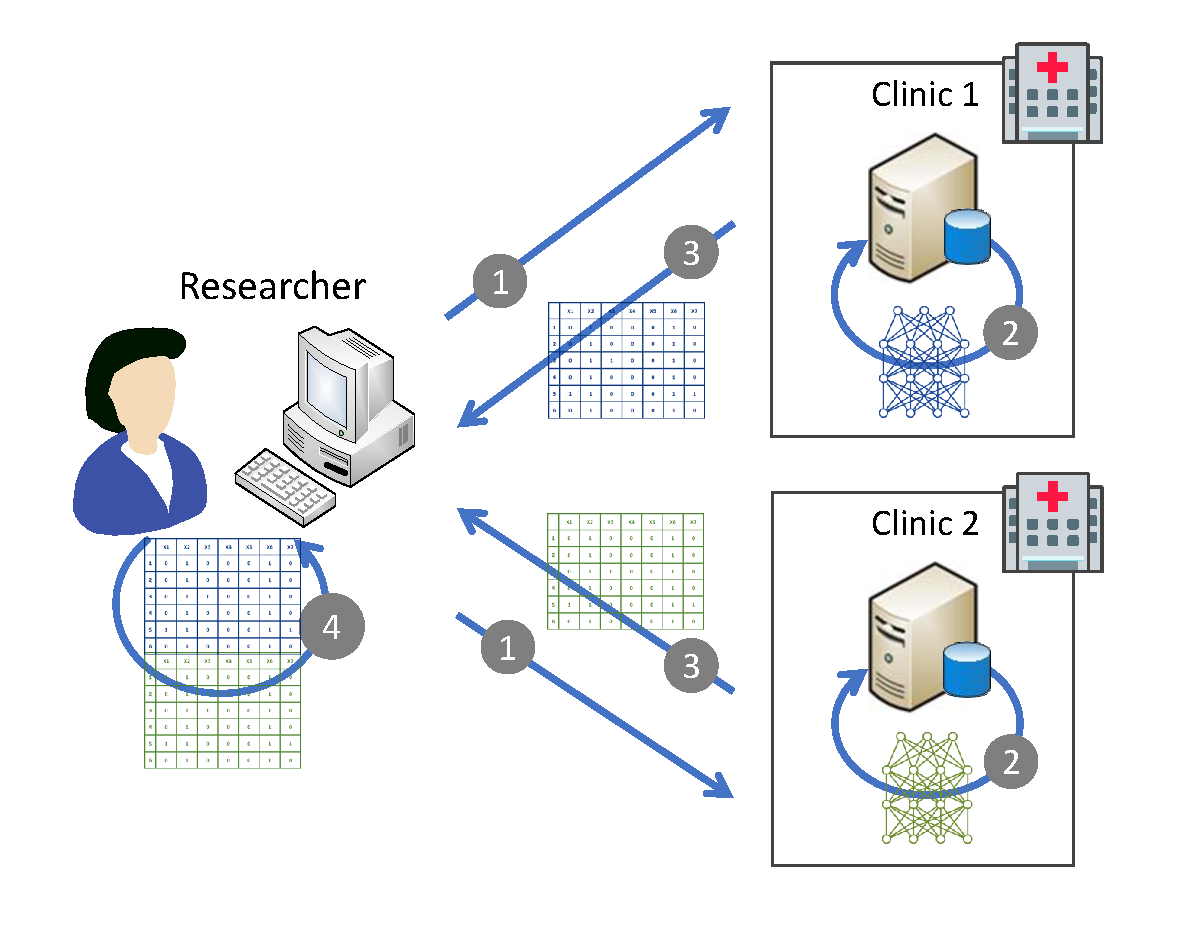
\includegraphics[scale=0.7]{images/synthetic_data_principle.pdf}
   \caption{Working with synthetic data in a distributed setting. \circlenum{1}The researcher asks the different participating sites for synthetic data. \circlenum{2}The sites fit generative models on their local data sets and \circlenum{3} return synthetic data that are generated by the models to the researcher. \circlenum{4}The researcher can conduct arbitrary analyses on the combined synthetic data.}
   \label{fig:syntheticdataprinciple}
 \end{figure}

\subsubsection{Different generative approaches}\label{diffgenmodels}

For creating synthetic data, any generative approach can be used.
In addition to DBMs, which are the main focus of this work, other approaches, in particular other types of neural networks, shall be considered as well.
Two recent approaches, which have gained much popularity in the last years, are {\em variational autoencoders} (VAEs) \citep{Kingma2013} and {\em generative adversarial networks} (GANs) \citep{goodfellow_generative_2014}.
What distinguishes these models from DBMs is that they are feed-forward neural networks.
In contrast to DBMs, where all nodes in the graph influence all of their neighbors in the graph, the activation in VAEs and GANs flows only in one direction.
This has the advantage that VAEs and GANs can be trained via the backpropagation algorithm \citep{backpropagation}, which is supported by many deep learning frameworks.
The implementation of VAEs and GANs that is used for the experiments here is based on the Julia package \apkg{Flux}.

In addition to the complex neural network models, also simpler techniques shall be included in the experiments to be able to see whether more complex models really bring an improvement.

{\em Multiple imputation by chained equations} (MICE) is a technique that is primarily used for imputing missing values in data sets \citep{mice}.
The algorithm can also be used as a generative approach because generating new data can be considered to be equivalent to imputing whole samples.
The algorithm for fitting a MICE model as a generative model on binary data consists of the following steps \citep{goncalves, dsdbm}:
\begin{enumerate}
\item Define a random order of the variables. This may be different from their original ordering. The variables in this order are denoted as $v_1, \dots, v_n$.
\item Estimate the empirical distribution $\hat{p}_1$ of $v_1$. For a binary variable, this means calculating the mean value $\hat{\mu}_1$ of $v_1$.
\item Fit logistic regression models $R_2, \dots, R_n$, with model $R_i$ predicting $v_i$ from  $v_1, \dots, v_{i-1}$. If adding variable $v_{i-1}$ leads to collinearity when estimating $R_i$, then $v_{i-1}$ is not used as independent variable in $R_{i}, \dots, R_n$. Furthermore, if $v_i$ is simply constant, then $R_i$ will predict this constant value without using other variables.
\end{enumerate}

From the MICE model $(\hat{p}_1, R_2, \dots, R_n)$, new samples $\tilde{v}_1, \dots , \tilde{v}_n$ can be generated as follows:

\begin{enumerate}
\item Sample $\tilde{v}_1$ from $\hat{p}_1$.
In the case of a Bernoulli distributed variable, this means to sample $\tilde{v}_1$ from a Bernoulli distribution with $p(\tilde{v}_1 = 1) = \hat{\mu}_1$.
\item For  $i \in 2, \dots, n$: Sample $\tilde{v}_i$ using the prediction of the regression model $R_i$ from the previously sampled values, with $p(\tilde{v}_i = 1) = R_i(\tilde{v}_2, \dots, \tilde{v}_n)$.
\end{enumerate}

By predicting variables from another, the MICE model aims to capture the association between the variables.

Like in \cite{goncalves}, the method of {\em independent marginals} (IM) is considered as the simplest approach for comparison.
This approach does not aim at modeling the association of the variables and treats them independently.
For IM, the empirical distribution of each variable is calculated separately.
Each variable is then sampled independently from the other variables according to its empirical marginal distribution.
For Bernoulli distributed variables, this means to create synthetic samples using the estimated marginal means of the variables, as described above in the algorithm of the MICE method, where this is only used for sampling the first variable.
With this, the IM method provides a baseline reference for the comparison of the different approaches.

\subsubsection{Measuring performance}\label{measuringperformance}
For comparing the generative performance of different generative models, measures for the quality of the generated data are needed.
For imaging data, visual inspection of samples is often used  to demonstrate the quality of the model.
A model that has been trained on images of human faces and that generates diverse faces which are not too close to the original input faces can be regarded as a good model.
For this purpose, generated images and the closest input images are displayed next to each other \citep{theis_note_2015}.
In such a case, a numeric score for measuring the quality is not necessary because the usefulness of the model becomes apparent.
In case of patient records or genetic variant data, assessing the quality of synthetic data is not so simple because the human eye and brain is not equipped in the same way to judge whether patient records or genetic variant data are proper samples of the input distribution and are, at the same time, not too close to original samples.

One possibility for allowing a visual inspection of generated data, however, is to use a clustering approach \citep{hclust}.
With similar records grouped together, the clustered data can be plotted and emerging patterns can be inspected visually.
This is a common visualization technique for inspecting omics data \citep{eisen_cluster_1998}.
The similarity of patterns between original and synthetic data can be compared by putting clustered views of these data sets next to each other.

Still, measuring the performance with a numeric measure has the advantage that different models can be evaluated automatically and that the assessment is less subjective than with the visual inspection of samples.
There are many different measures, which can be used to evaluate the performance of generative models and which also have been applied to medical data sets \citep{goncalves}.

The odds ratio is a measure for the bivariate association between two binary variables \citep{blandaltmannodds}.
For the experiments here, the rooted mean squared error (RMSE) between the pairwise log odds ratios is utilized as a performance metric \citep{nussberger_synthetic_2020}.
Given a validation data set $x_{val}$ and a generated data set $x_{gen}$, this metric is calculated as follows:
For each of the two data sets, the pairwise odds ratios are calculated for all pairs of variables in the respective data set.
These values are logarithmized and collected in matrices.
(If zeros occur in cells of the cross tables for calculating the odds ratios, a value of 0.5 is used for these cells instead to avoid getting infinite values.)
Due to the symmetry of the matrices, only the lower half is used to calculate the Euclidean distance between the two matrices.
The resulting value for the Euclidean distance of the lower half of the matrices is defined as the distance measure $d(x_{gen}, x_{val})$ for the pairwise log odds ratios, which shall be used here to compare different generative approaches.


\subsubsection{Measuring disclosure}\label{measuringdisclosure}

In addition to the utility of the approaches, their disclosure risk shall also be examined and compared.
For this, the focus lies on membership privacy (see \ref{privacyconcepts}).
Applying differential privacy like \cite{abadi_deep_2016} would require to change the learning procedure, which would in turn affect the utility \citep{hayes_logan_2019}.
Additionally, changing the learning procedure may affect different learning algorithms in a different way, which could make it difficult to compare the models fairly.
Therefore, two simpler approaches are used here to assess the disclosure risk instead.

\paragraph{Simulating a membership attack}\label{membershipattack}
A method for measuring disclosure is to simulate a membership attack \citep{choi_generating_2017, goncalves}.
The attacker has a set of synthetic data and a set of ``real'' samples , which are referred to as ``test'' samples for this experiment.
The attacker then guesses whether one of the test samples is in the training set of the model that generated the synthetic data set or not.
The precision and sensitivity of the guesses are reported as outcome of the experiment.

The guesses of the attacker are based on distances between samples.
The attacker assumes that one of the test samples is in the training data set if the test sample is near a synthetic sample, i.e., if the distance with respect to some distance measure is lower than a pre-specified threshold.
As distance measure between two samples, the absolute-value norm is used, which is equivalent to the Hamming distance for binary values.
For each of the training samples, the attacker may identify the sample as training sample if there is a synthetic sample nearby (true positive), or the attacker may guess wrong if no synthetic sample is inside the pre-specified distance (false negative).
Also, for each test sample, the attacker may guess correctly that it has not been used for training (true negative) or assume that it is in the training set (false positive).

Based on the chosen distance, different values for precision and sensitivity result from the experiment.
Since a best value for the distance threshold cannot be determined, different distances are used, and multiple outcomes are reported.
The size of the test data set is chosen to be equal to the size of the training data set.
Consequently, a value of 0.5 as outcome indicates that the synthetic data is not informative for the attacker. 

\subsection{The proportion of overfitting as a new disclosure metric}\label{proportionoverfitting}

Another way of assessing disclosure is to inspect the overfitting of a model.
This is the case because overfitting happens if a model learns the peculiarities of the training data rather than generalizable patterns.
The more the model captures information about the individuals in the training data rather than information that applies to all individuals in the basic population, the more likely it is that an attacker can conclude that a specific individual was used in the training data from comparing this individual with synthetic individuals in contrast to other individuals in the basic population.
Therefore, overfitting has a direct relation to membership privacy.
Overfitting has also been investigated as an indicator for disclosure risk in synthetic images \citep{webster_detecting_2019, hayes_logan_2019}.
The most extreme case of overfitting is if a model directly memorizes the original data and generates samples that are copies of training samples.
Such a case is an obvious violation of privacy.
But for most cases, the decision about a possible disclosure is not easily made in a binary way, and for those a numeric measure is needed.
Here, overfitting is measured using the training data set $x_{train}$, a validation data set $x_{val}$, a generated synthetic data set $x_{gen}$, and a similarity measure.
For the latter, the distance measure $d$, which is also used for measuring the performance (see \ref{measuringperformance}), can be used.
With this, the {\em proportion of overfitting} is defined as

\begin{equation}
\frac{d(x_{gen}, x_{val}) - d(x_{gen}, x_{train})}{d(x_{gen}, x_{val})}.
\end{equation}

This proportion grows if the similarity  between the generated data and the training data increases relative to the similarity between the validation data and the generated data.


\subsection{An experiment with simulated genetic variant data}\label{simuexp}

This experiment investigates whether the approach of generating data in a distributed manner across different sites, as depicted in Figure \ref{fig:syntheticdataprinciple}, is feasible using DBMs.
In particular, I investigate how the number of participating sites and the numbers of samples at each sites influence the quality of the synthetic data.

The experiment is based on simulated genetic variant data with patterns that are clearly visible in a binary heatmap with a hierarchical clustering \citep{hclust} of the  samples.
With these clearly visible patterns it is possible to evaluate the synthetic samples visually by judging whether the original patterns can be recovered in the synthetic data.


\subsubsection{Experimental setup}\label{simuexpsetup}

In the experiment a single simulated data set is distributed equally across different sites.
Figure \ref{fig:experimentalsetup} shows the different steps of the experiment.


\begin{figure}[h]
   \centering
   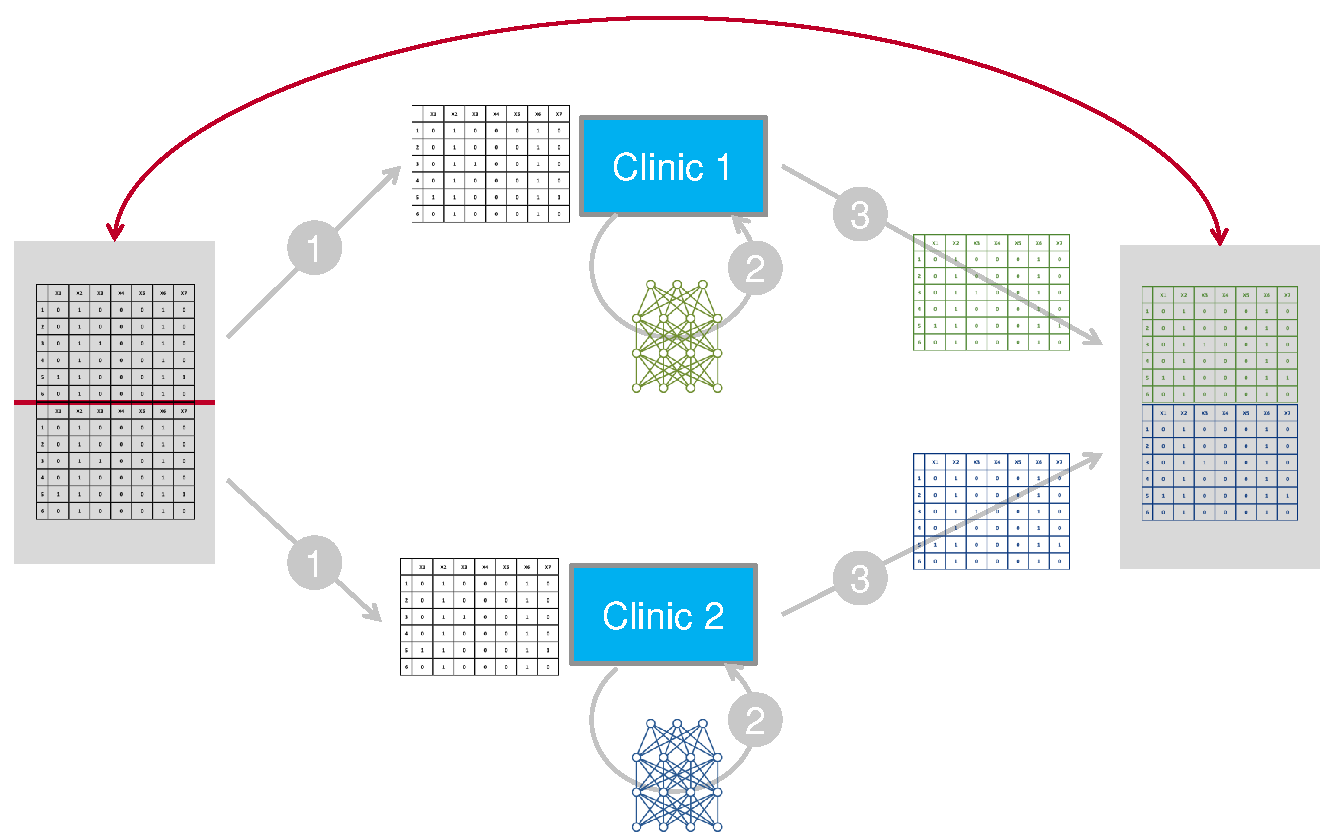
\includegraphics[scale=0.7]{images/experimentalsetup.pdf}
   \caption{Sketch of the experimental setup.
    \circlenum{1} The original data is split onto the different sites. To keep it simple, there are only two sites depicted here.
    \circlenum{2} Generative models are trained at the different sites using their share of the data.
    \circlenum{3} These models generate synthetic data, which are combined into a single synthetic data set. (The generated data sets are of the same size as the respective training sets.)
    \circlenum{4} The original and the combined synthetic data set are compared.}
   \label{fig:experimentalsetup}
 \end{figure}

The simulated data are inspired by genetic variant data, more specifically, single nucleotide polymorphisms (SNPs).
In SNP data, each variable stands for a defined location on a chromosome and the values indicate whether the sample deviates from a defined reference genome at this location.
There are 50 binary variables in the simulated data set.
The 500 samples in the data set are split into ``cases" and ``controls" in a ratio of 1:1.
In all 50 variables, the ``control" samples consist of independently sampled binary values, which are set to 1 with a probability of 0.1.
The ``cases" differ from this in 5 groups of 5 SNP variables.
There are 5 disjoint subgroups among the cases, which have all values set to 1 in either the variables 1-5, or 10-15, or 20-25, or 30-35, or 40-45.
In all other variables, the ``cases" follow the same distribution as the ``controls".
As a motivation behind the properties of the simulation data set, one can consider the following:
If a group like the groups of 5 SNP variables is present in patients with a certain condition (``cases"), this could indicate that these mutations must occur together to activate or deactivate certain genetic pathways, thereby leading to the condition.


\subsubsection{Results}\label{simuexpresults}

A hierarchical clustering view of the data is shown in Figure \ref{fig:distclustersnps}, panel A.
The most obvious structures there are the black blocks.
These result from the five subgroups in the ``cases'' as the hierarchical clustering algorithms manages to group those samples together.
In the original data, these black blocks are very solid as all samples in each subgroup are assigned to one cluster.

 \begin{figure}[!hb]
   \centering
   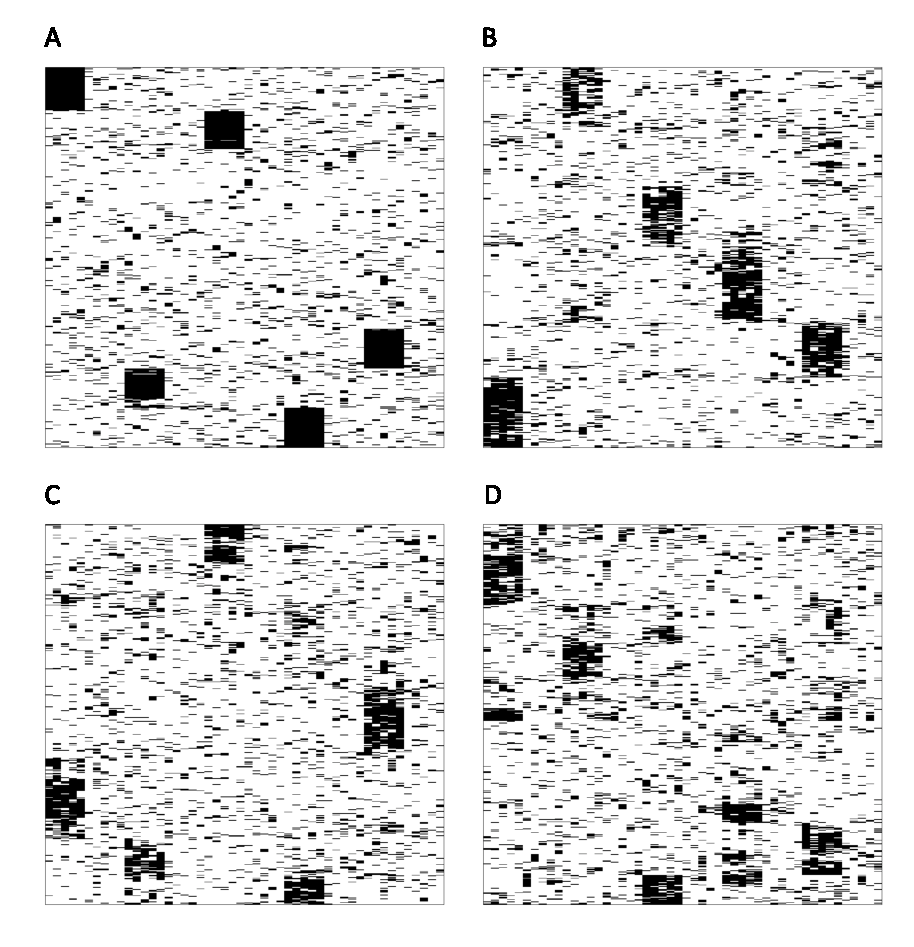
\includegraphics[scale=1]{images/hclust.pdf}
   \caption{Comparison of original (simulated) data and synthetic data. The samples, which are depicted in the rows of the matrices, are clustered hierarchically based on their Euclidean distances. The columns are the different SNPs/variables. Black rectangles indicate values of 1, white rectangles values of zero. The black blocks result from the groups of five 1s, as samples with the same pattern are clustered together. The different vertical positions of the blocks result from the noise outside of the pattern, which randomly influences the clustering. A: original data set. B: synthetic data generated from a DBM trained on the original data set. C and D: synthetic data from the distributed experiment with 2 and 20 sites, respectively.}
   \label{fig:distclustersnps}
 \end{figure}

It has to be noted that the vertical position of the black blocks is irrelevant because also the noise outside of the patterns influences the clustering of the samples and thus determines the vertical positions of the blocks.
The horizontal position of the blocks, however, is determined by the positions of the 5 co-occuring SNP variables and these are the same across all panels.

Different synthetic data sets are depicted in panels B, C and D.
From panel B, where synthetic data from a single DBM is shown, one can see that using synthetic data instead of the original data leads to some bias, as the black blocks are not as dense as in the original data, which means that there is some additional noise in the generated synthetic data.
Nevertheless, it is clearly visible in the synthetic data that there is a strong correlation between the specific variables in subgroups of samples.
This shows that a DBM is able to learn such patterns.
When the data is split between different sites/DBMs as shown in Figure \ref{fig:experimentalsetup}, the blocks become less clear and the noise increases.
Panel D shows an extreme case, where there are 20 sites with only 25 samples per site.
Still, blocks in the respective variables are visible.
But the noise outside of the blocks is captured less well, and artifacts from noise increase as the model has fewer samples to learn from.

The employed DBMs had two hidden layers with 50 and 10 hidden nodes.
A learning rate of 0.001 was used for pre-training and a initial learning rate of 0.1 was used for fine-tuning.
Both pre-training and fine-tuning were performed for 30 training epochs.

Summed up, the results of the experiment indicate that using DBMs on distributed data for generating synthetic data (see Figure \ref{fig:syntheticdataprinciple} in \ref{syntheticdata_ds}) can be a suitable approach for analyzing higher-level patterns in data.

\FloatBarrier
\subsection{An experiment for comparing different distributed generative approaches on real genetic variant data}\label{realexp}

After the experiment with simulated data, the question remains how well the findings generalize to real genetic data.
It is also interesting how DBMs compare to other generative models, in particular, in settings of small sample size.
Therefore, the next experiment evaluates DBMs and other generative approaches in a setting similar to the one in Section \ref{simuexp} using real genetic variant data that is distributed among a number of virtual sites.
As additional generative approaches, VAEs, GANs and MICE are considered.
The method of independent marginals is added as a reference for a baseline performance.

The complete code for reproducing this experiment can be found on GitHub\footnote{\url{https://github.com/stefan-m-lenz/dist-gen-comp/}}.
There, the Julia package \apkg{BoltzmannMachines} provides the DBM implementation.
VAEs and GANs are trained via the \apkg{Flux} Julia package in the same way as done by \cite{nussberger_synthetic_2020}. MICE also is implemented directly in Julia, using the Julia package \apkg{GLM} \citep{juliaglm} for logistic regression.

\subsubsection{Experimental setup}\label{realexpsetup}

The data for the experiment is taken from the 1000 genomes project \citep{1000genomes}.
More specifically, a subset of the 1000 genomes data is used, which is available online from a web page \citep{impute_1000_genomes} of the IMPUTE2 software \citep{impute2}.
This data set contains genetic variant data (SNP data) of 2504 humans.
The data is provided in haploid form, that is, the information about the genetic variation is given on the level of the chromosomes.
In the data there are in total 5008 chromosomes, which are used as independent samples for the purpose of learning structure in genetic data.
Each of these samples is a vector of binary SNP variables.
Each variable stands for a defined location on a chromosome, with a value of 1 indicating that the sample has a defined deviation from the reference genome in this place.
Such a deviation is also referred to as the minor allele.

From the complete genetic information, 30 loci on chromosome 6, spanning 50 SNP variables, are randomly selected.
As the variance in some SNPs across samples is very low, only SNPs with a minor allele frequency above 0.2 were considered.
This prevents that the structure in the data sets becomes too simple by excluding variables that are expected to be mostly constant in subsets of samples.
For each of these 30 different genomic locations, a training data set $x_{train}$, a test data set $x_{test}$, and a validation data set $x_{val}$ are selected.
From the 5008 samples, 500 samples are used in the training data sets, 100 in the test data sets, and 1000 in the validation data sets.

To evaluate different generative approaches in a distributed setting,
the setup of the experiment is very similar to the one with the simulated data shown in Section \ref{simuexp}.
In the same way as described in \ref{simuexpsetup} and shown in Figure \ref{fig:experimentalsetup},
the training data is distributed among different sites, and then different models are trained at the sites on their share of the data.
Further, the models at the different sites generate synthetic data, which are then compiled into a joint synthetic data set.
The joint synthetic data sets are finally used for the evaluation.

As generative approaches, DBMs, VAEs, GANs, MICE and IM are considered (see \ref{diffgenmodels}).
The network architecture of DBMs, VAEs, and GANs is chosen to be similar.
For DBMs, VAEs, and GANs, the number of training epochs and the random initialization of the model parameters are subject to hyperparameter optimization.
The best models are found via a grid search, which includes up to 2000 training epochs and 15 different seeds for the random number generator.
For MICE, also 15 different orderings of the variables are explored.

To have a fair comparison between the approaches, the same performance metric must be used for picking the best model per approach as for the overall comparison.
For this purpose, only a measure that applies to the synthetic data can be used, as the different approaches have different optimization criteria.
GANs, in particular, do not even have a single optimization criterion because the discriminator and generator networks have different loss functions.
Therefore, a measure of the quality of the synthetic data is needed for comparing the models as well as for picking the model with the best performance for each approach.
Here, the rooted mean squared error (RMSE) of the log odds ratios is employed as this performance measure (see \ref{measuringperformance}).

For the models with the best performance, the disclosure risk of the generated data is also assessed.
This is done via the proportions of overfitting (see \ref{proportionoverfitting}) and simulated membership attacks (see \ref{membershipattack}).
The test data sets for the simulated membership attacks comprise 500 samples from the respective validation data sets.

\FloatBarrier
\subsubsection{Results}\label{realexpresults}

\paragraph{Generative performance}
The results of the comparison with respect to the generative performance of the different approaches are shown in Figure \ref{fig:rmseodds} and Table \ref{tab:distgenresults_rmse}.
There, the distance $d(x_{gen},x_{val})$, which has been defined in \ref{measuringperformance}, is used as performance metric.
This distance measures how well the bivariate associations between all combinations of variables in the original data are preserved in the synthetic data.
The effect of the sample size and the number of participating sites can be seen by comparing the results for using the whole data set (``One site''), and splitting the data on 2, 5, and 20 sites.
By splitting the data, the number of samples per site decreases from 500 to 250, 100, and 25, respectively.

Running the complete experiment took 25 hours on a cluster of three computers with 8, 12, and 28 cores with clock speeds of about 3 GHz and at least than 8 GB RAM per core.

The median performance of DBMs and VAEs is very close, especially in the settings with one and two sites (see Figure \ref{fig:rmseodds} and Table \ref{tab:distgenresults_rmse}).
The other approaches perform clearly worse in all scenarios.
As IM does not aim at modeling the bivariate associations, and MICE is not clearly better than IM, it can be concluded that MICE also mostly fails to capture the overall structure of the bivariate assiciations.
In the setting with one site and 500 samples, the GAN is at least somewhat better than the simpler approaches, IM and MICE.
The limited sample size seems to be especially impacting GANs negatively, as the performance becomes equally bad to IM and MICE in the other settings with split data.

In the settings with 5 and 20 sites, the variance in the performance of DBMs gets higher.
The variance of the performance of VAEs stays very constant across all the scenarios.

\paragraph{Disclosure risk}
With lower sample size, the question of the disclosure risk becomes more critical, as the danger of copying data increases.
I am first measuring the disclosure risk by evaluating the proportion of overfitting as defined in \ref{proportionoverfitting}.
The results for this evaluation can be found in Figure \ref{fig:distgenresults_overfitting} and Table \ref{tab:distgenresults_overfitting}.
There, the same models as shown in Figure \ref{fig:rmseodds} are evaluated with respect to disclosure.

It can be seen that DBMs exhibit less overfitting than VAEs and GANs here.
In the scenarios with two and five sites, they even overfit less than all the other approaches.
In the extreme scenario with 20 sites with 25 samples, the overfitting is similarly pronounced in all approaches.
With a decreased number of samples, the variance of the overfitting increases. This can simply be explained by the fact that if fewer samples are in the data set, they may not always represent the overall structure well.

For the same models as used for assessing the overfitting, the disclosure risk is also appraised via simulated membership attacks as described in \ref{membershipattack}.
The precision and sensitivity of the membership attacks are shown in Figure \ref{fig:membershipattack}.

To interpret the values for precision and sensitivity, one can consider the following:
As the training and test data set for the membership attacks have equal size, a precision of 0.5 is expected for a random guess.
Models generating synthetic data that cannot be used by the attacker to infer membership should therefore also have a precision that is close to 0.5.
A higher precision results from models generating samples that are nearer to training samples.
A low precision can correspond to a low sensitivity, as can be seen in Figure \ref{fig:membershipattack}.
The sensitivity can be seen as a performance metric on the training data here because it quantifies the overall distance between synthetic samples and training samples.
Therefore, a very low sensitivity means that the synthetic samples are too far away from the training samples.
This in turn may result in a precision that is lower than 0.5 because the attacker is simply mislead by synthetic data of bad quality.
If a model produces data that is so different from the training data that no true positives or false positives can be found by the attacker, no value for the precision can be determined.

For DBMs and VAEs, the values for the precision are very close to 0.5 across all settings.
This means that no disclosure risk can be detected by this method in DBMs and VAEs.
VAEs have a slightly higher sensitivity than DBMs, indicating a slightly better performance on the training data, which is in line with the higher overfitting of VAEs compared to DBMs here.
The variance of the precision of the membership attack on GANs becomes higher with an  increasing number of sites and a decreasing number of samples.
This corresponds to an increasingly worse performance of GANs there, which can also be seen in the lower sensitivity values.
MICE and IM also have clearly lower sensitivity values than DBMs and VAEs.


\noindent\begin{minipage}{\linewidth}
   \centering
   \captionsetup{type=figure}
   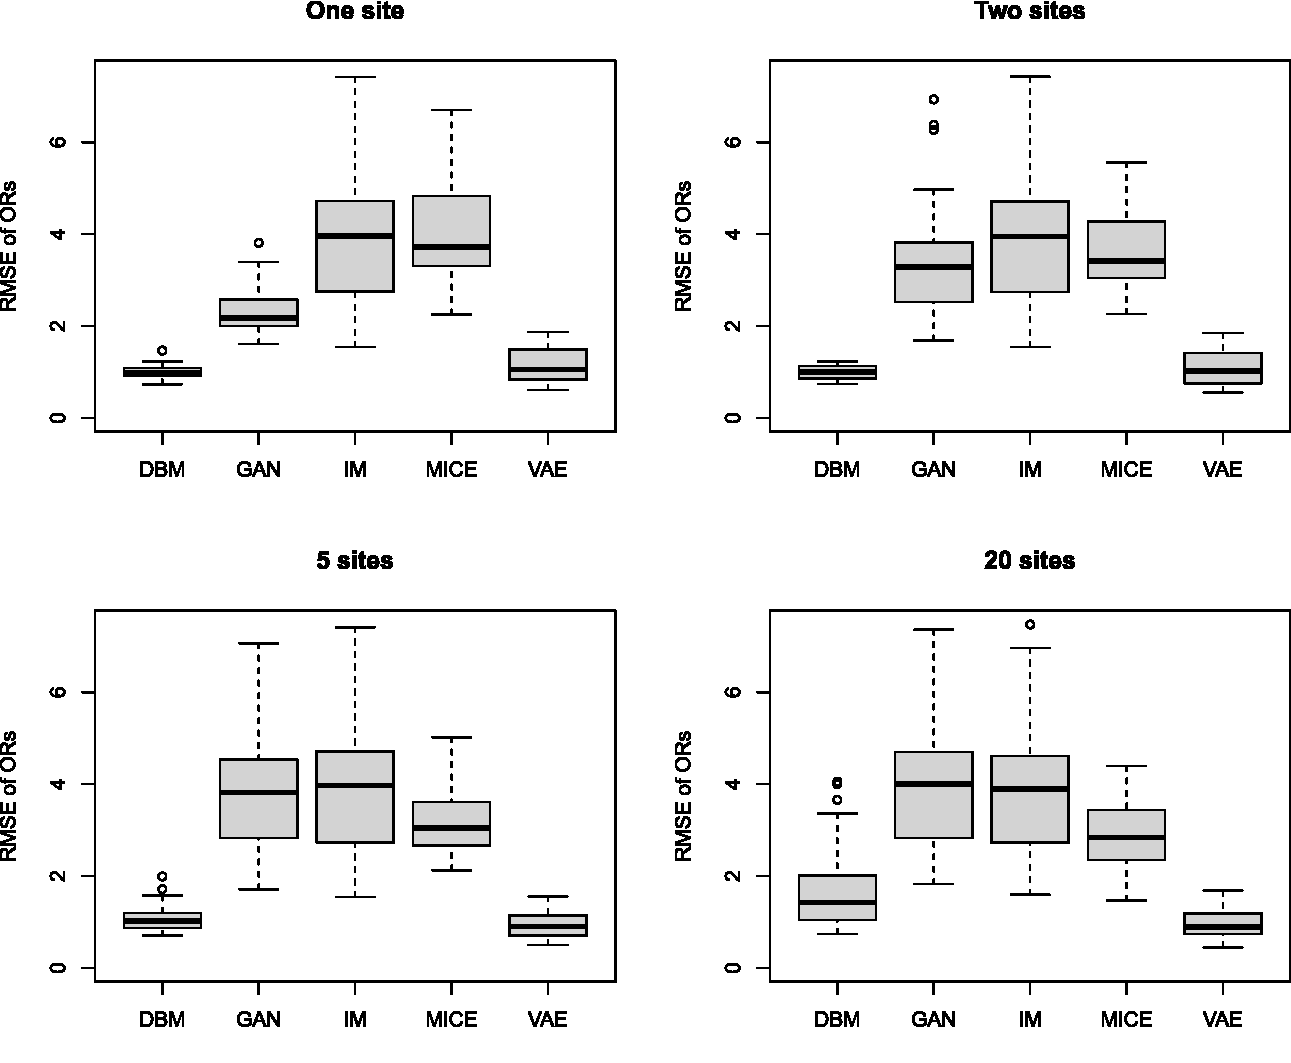
\includegraphics[scale=0.7]{images/rmseodds.pdf}
   \captionof{figure}{Comparing the generative performance of DBMs, GANs, IM, MICE, and VAEs via the RMSE of log odds ratios. There is one data point for each genomic locus in the box plots. (See \ref{realexpsetup} for the description of the data sets.)
   Separate for the different approaches, the data points in the plot show the performance of the best models with respect to the RMSE of log odds ratios that are found in the grid search.}
   \label{fig:rmseodds}


\captionsetup{type=table}
\captionof{table}{Quantiles of the RMSE of log odds ratios as depicted in Figure \ref{fig:rmseodds} summarized as: {\em Median} ({\em 5\% quantile} - {\em 95\% quantile}).}
\label{tab:distgenresults_rmse}
\begin{tabular}{l|cccc}
\\\\[-4\medskipamount]
& 1 site & 2 sites & 5 sites & 20 sites \\[0.5ex]
\hline
\\\\[-4\medskipamount]
DBM & \makecell{0.98 \\ (0.82 - 1.21)} & \makecell{1.00 \\ (0.78 - 1.19)} & \makecell{1.03 \\ (0.74 - 1.65)} & \makecell{1.42 \\ (0.89 - 3.85)} \\[2ex]
GAN & \makecell{2.17 \\ (1.86 - 3.36)} & \makecell{3.28 \\ (2.12 - 6.33)} & \makecell{3.82 \\ (2.41 - 6.41)} & \makecell{4.00 \\ (2.41 - 6.88)} \\[2ex]
IM & \makecell{3.96 \\ (2.33 - 6.95)} & \makecell{3.95 \\ (2.32 - 6.95)} & \makecell{3.97 \\ (2.32 - 6.95)} & \makecell{3.90 \\ (2.30 - 6.84)} \\[2ex]
MICE & \makecell{3.72 \\ (2.87 - 6.04)} & \makecell{3.41 \\ (2.76 - 5.13)} & \makecell{3.05 \\ (2.47 - 4.61)} & \makecell{2.84 \\ (1.93 - 4.22)} \\[2ex]
VAE & \makecell{1.05 \\ (0.72 - 1.85)} & \makecell{1.02 \\ (0.68 - 1.72)} & \makecell{0.90 \\ (0.61 - 1.50)} & \makecell{0.89 \\ (0.53 - 1.53)} \\[2ex]
\end{tabular}
\end{minipage}

\noindent\begin{minipage}{\linewidth}
   \centering
   \captionsetup{type=figure}
   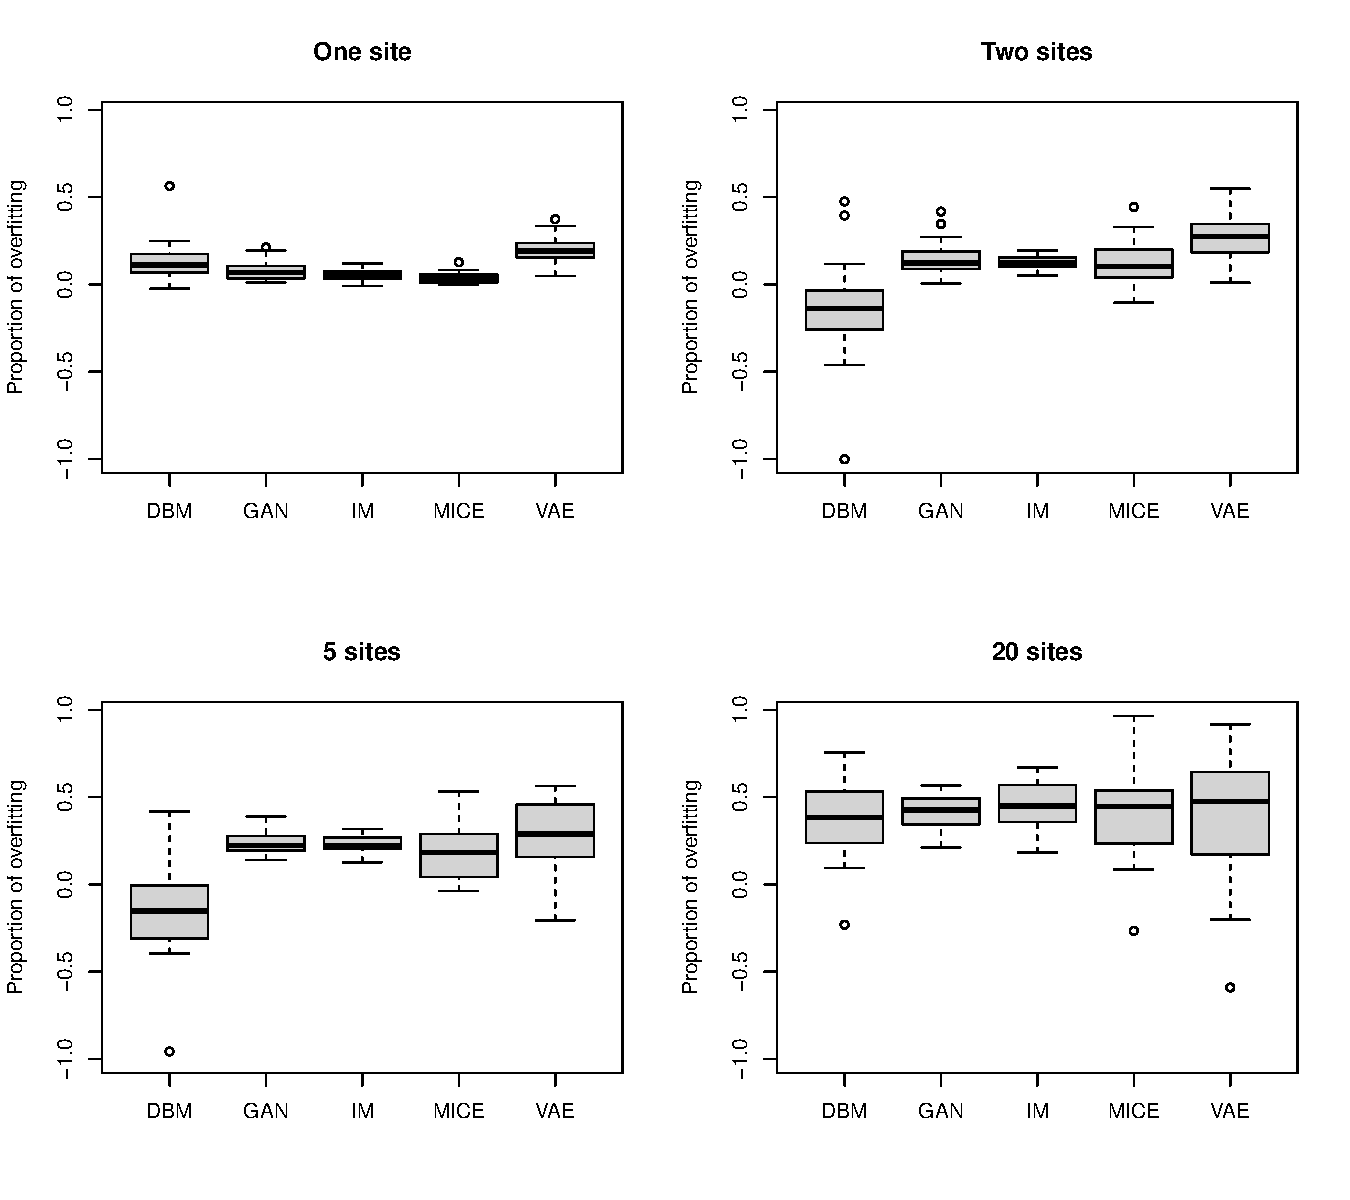
\includegraphics[scale=0.7]{images/overfitting.pdf}
   \captionof{figure}{Comparing the proportion of overfitting in DBMs, GANs, IM, MICE, and VAEs via the RMSE of log odds ratios in several settings of distributed data.
   The data points shown stand for the same data sets and models as in Figure \ref{fig:rmseodds}, i.e., there is one data point for the best model with respect to the RMSE of log odds ratios per genomic locus.}
   \label{fig:distgenresults_overfitting}

\captionsetup{type=table}
\caption{Quantiles of the proportion of overfitting as depicted in Figure \ref{fig:distgenresults_overfitting}, summarized as: {\em Median} ({\em 5\% quantile} - {\em 95\% quantile}).}\label{tab:distgenresults_overfitting}.
\begin{tabular}{l|cccc}
\\\\[-4\medskipamount]
& 1 site & 2 sites & 5 sites & 20 sites \\[0.5ex]
\hline
\\\\[-4\medskipamount]
DBM & \makecell{0.11 \\ (-0.016 - 0.24)} & \makecell{-0.14 \\ (-0.44 - 0.27)} & \makecell{-0.15 \\ (-0.39 - 0.24)} & \makecell{0.38 \\ (0.11 - 0.69)} \\[2ex]
GAN & \makecell{0.068 \\ (0.013 - 0.17)} & \makecell{0.12 \\ (0.018 - 0.31)} & \makecell{0.22 \\ (0.15 - 0.34)} & \makecell{0.43 \\ (0.29 - 0.55)} \\[2ex]
IM & \makecell{0.055 \\ (-0.0045 - 0.099)} & \makecell{0.12 \\ (0.058 - 0.18)} & \makecell{0.22 \\ (0.15 - 0.31)} & \makecell{0.45 \\ (0.30 - 0.63)} \\[2ex]
MICE & \makecell{0.031 \\ (0.0022 - 0.08)} & \makecell{0.10 \\ (0.0048 - 0.32)} & \makecell{0.18 \\ (-0.019 - 0.45)} & \makecell{0.45 \\ (0.09 - 0.85)} \\[2ex]
VAE & \makecell{0.19 \\ (0.057 - 0.32)} & \makecell{0.27 \\ (0.062 - 0.45)} & \makecell{0.29 \\ (0.064 - 0.56)} & \makecell{0.48 \\ (-0.20 - 0.82)} \\[2ex]
\end{tabular}
\end{minipage}


\begin{figure}[h]
\centering
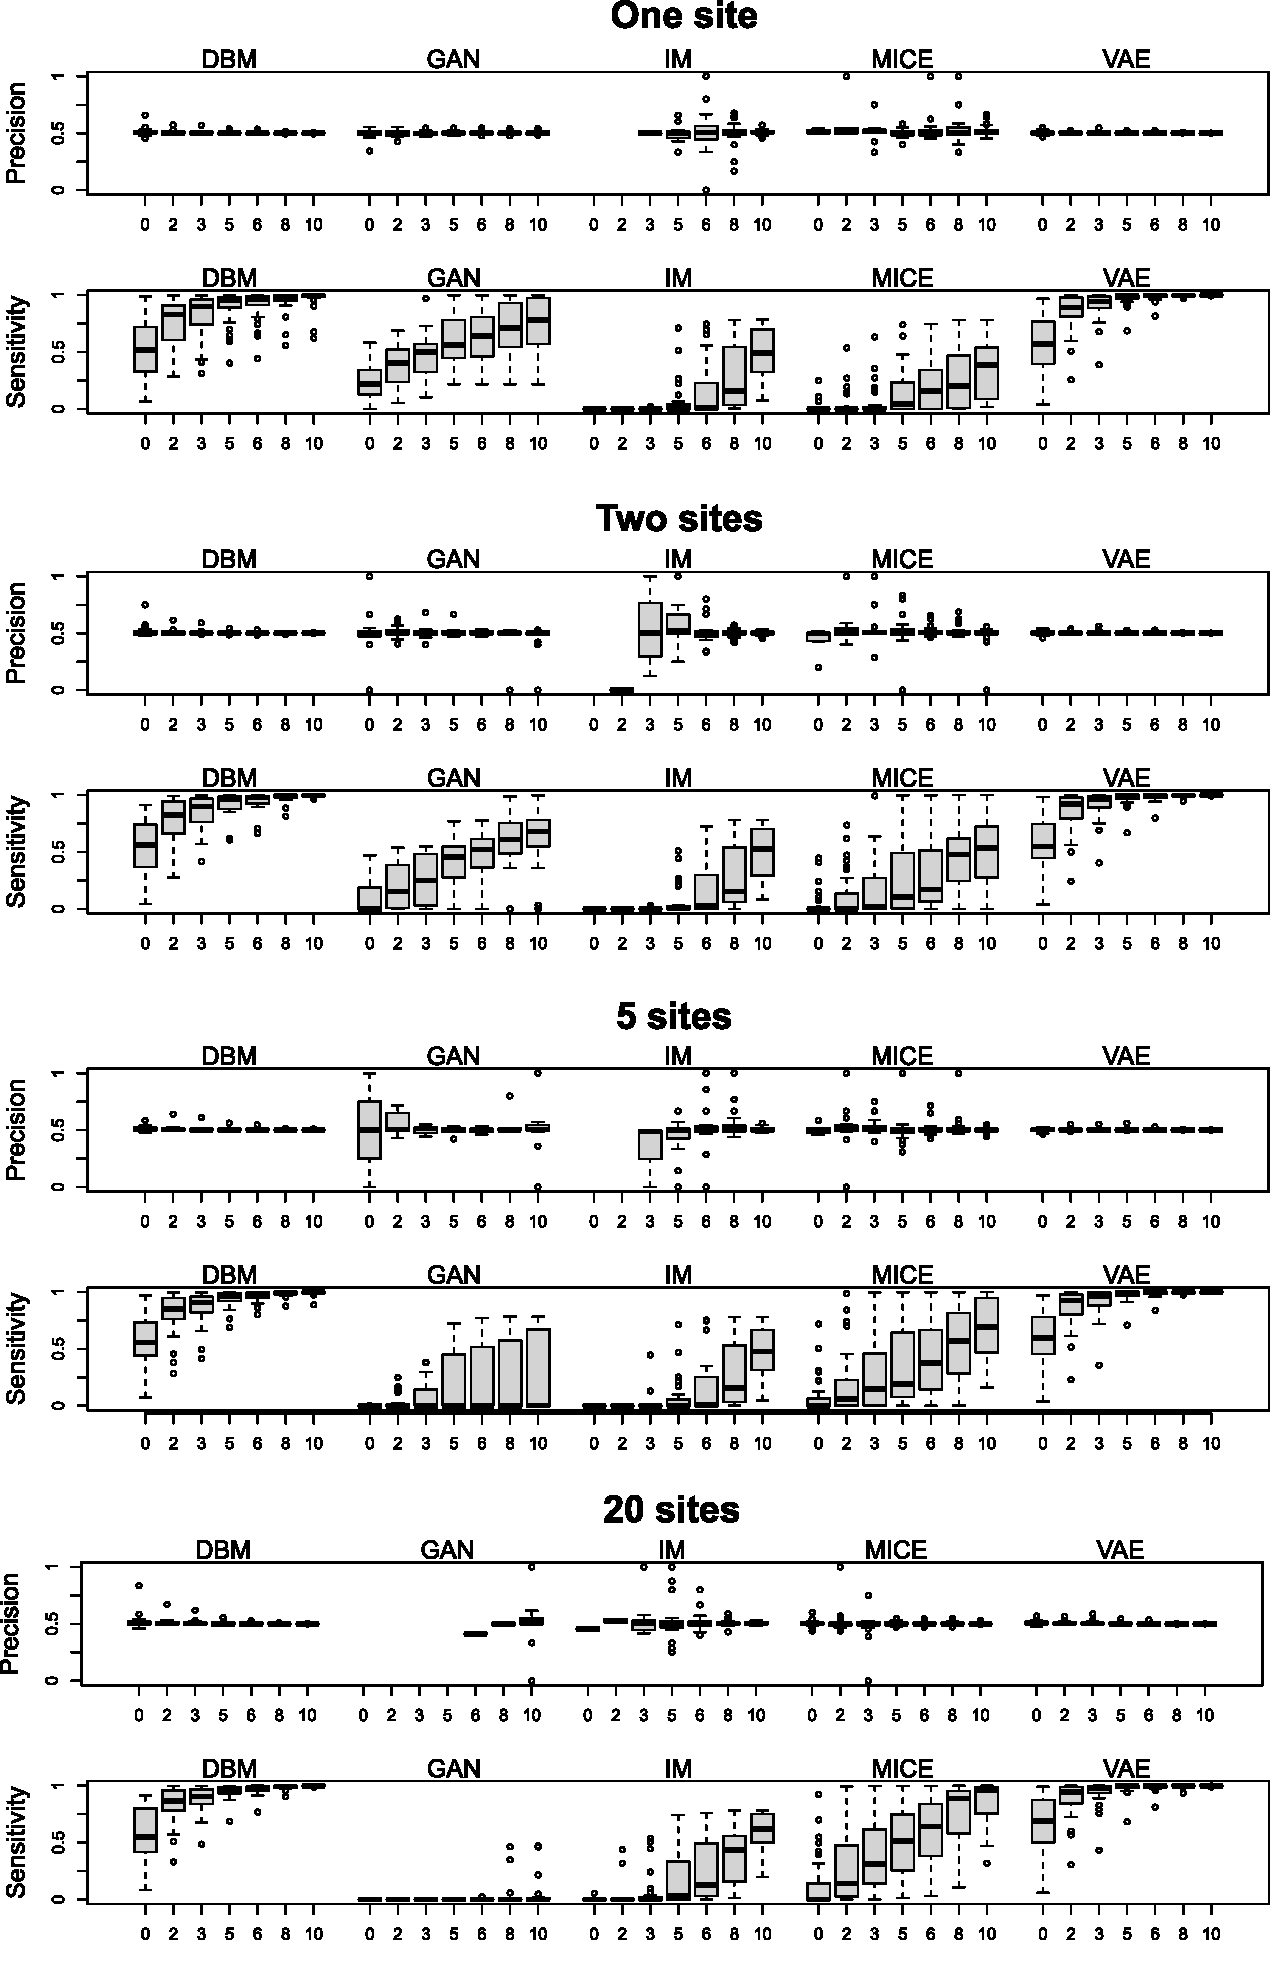
\includegraphics[scale=0.7]{images/membership_combined.pdf}
\caption{Precision and sensitivity of simulated membership attacks.  The data points shown stand for the same data sets and models as in Figure \ref{fig:rmseodds} and Figure \ref{fig:distgenresults_overfitting}. The x-axes indicate different distances used by the attacker (see \ref{membershipattack}).}
\label{fig:membershipattack}
\end{figure}



\FloatBarrier
\subsection{The \apkg{dsBoltzmannMachines} DataSHIELD package}\label{dsBoltzmannMachinesImpl}

The previous experiments in \ref{simuexp} and \ref{realexp} have investigated the feasibility of using synthetic data for joint analyses of distributed data.
In \ref{simuexp}, a hierarchical clustering was performed as a joint analysis.
The subsequent experiment in \ref{realexp} compares odds ratios in the synthetic data with odds ratios in the original data.
This comparison can be interpreted as an indicator for how well the synthetic data can be used in analyses like logistic regression models because odds ratios and logistic regression models are closely linked \citep{blandaltmannodds}.

Now a practical implementation of working with synthetic data in a distributed setting is presented on the basis of DBMs in DataSHIELD.
The resulting software is the first that allows generating synthetic data in DataSHIELD using deep learning.
The general principle for this has been sketched in Figure \ref{fig:syntheticdataprinciple}.
In Figure \ref{fig:examplaryworkflow}, the workflow using the software is shown in more detail using a single site.

\begin{figure}[h]
   \centering
   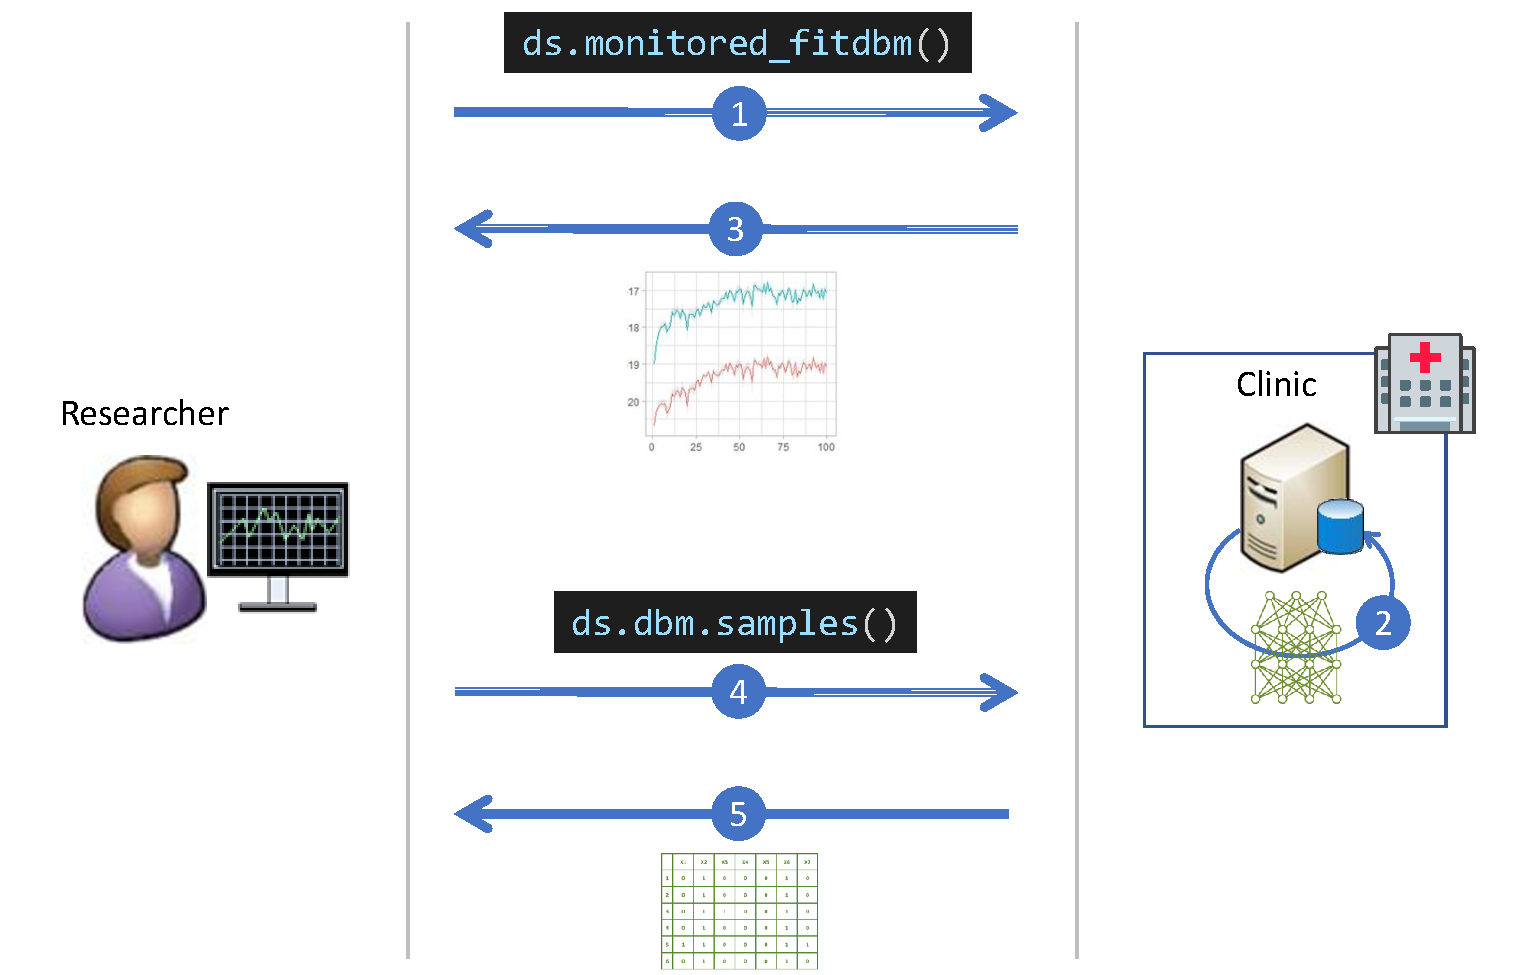
\includegraphics[scale=0.5]{images/dsBoltzmannWorkflow.pdf}
   \caption{Exemplary workflow for using the \apkg{dsBoltzmannMachines} package.
   \circlenum{1} The researcher calls a function for fitting a model, here a DBM, using a DataSHIELD analysis client with the client side of the software installed.
   \circlenum{2} The model is trained at the site using the server-side part of the software. During the training, the training can be monitored.
   \circlenum{3} This evaluation data can be returned to the researcher because it does not contain information about individuals.
   For finding good hyperparameters, these steps may be repeated several times.
   \circlenum{4} If the researcher is satisfied with a model, he/she can request samples from a model.
   \circlenum{5} The requested synthetic data is then returned to the researcher.}
   \label{fig:examplaryworkflow}
 \end{figure}

As indicated in Figure \ref{fig:examplaryworkflow}, the software consists of a client-side part and a server-side part.
These are implemented in two separate R packages, \apkg{dsBoltzmannMachinesClient}\footnote{\url{https://github.com/stefan-m-lenz/dsBoltzmannMachinesClient}} and \apkg{dsBoltzmannMachines}\footnote{\url{https://github.com/stefan-m-lenz/dsBoltzmannMachines}}.
The dependencies of all the parts are shown in Figure \ref{fig:dsBoltzmann_dependencies}.
Plots from the monitoring data are produced by a separate package, \apkg{BoltzmannMachinesRPlots}\footnote{\url{https://github.com/stefan-m-lenz/BoltzmannMachinesRPlots}}, which utilizes the \apkg{ggplot2} \citep{ggplot2} package.
Separating this functionality has the advantage that this package can also be used directly with the \apkg{BoltzmannMachines} Julia package in R via the \apkg{JuliaConnectoR} without DataSHIELD (see Section \ref{juliaconnectorDbmexample}).
For the communication with the Opal server, the Opal R client package is used, which can access functions that have been installed in a remote Opal server.
The functions on the server side are packaged in the \apkg{dsBoltzmannMachines} package.
These wrap the functionality of the \apkg{BoltzmannMachines} Julia package via the \apkg{JuliaConnectoR}.

\begin{figure}[h]
   \centering
   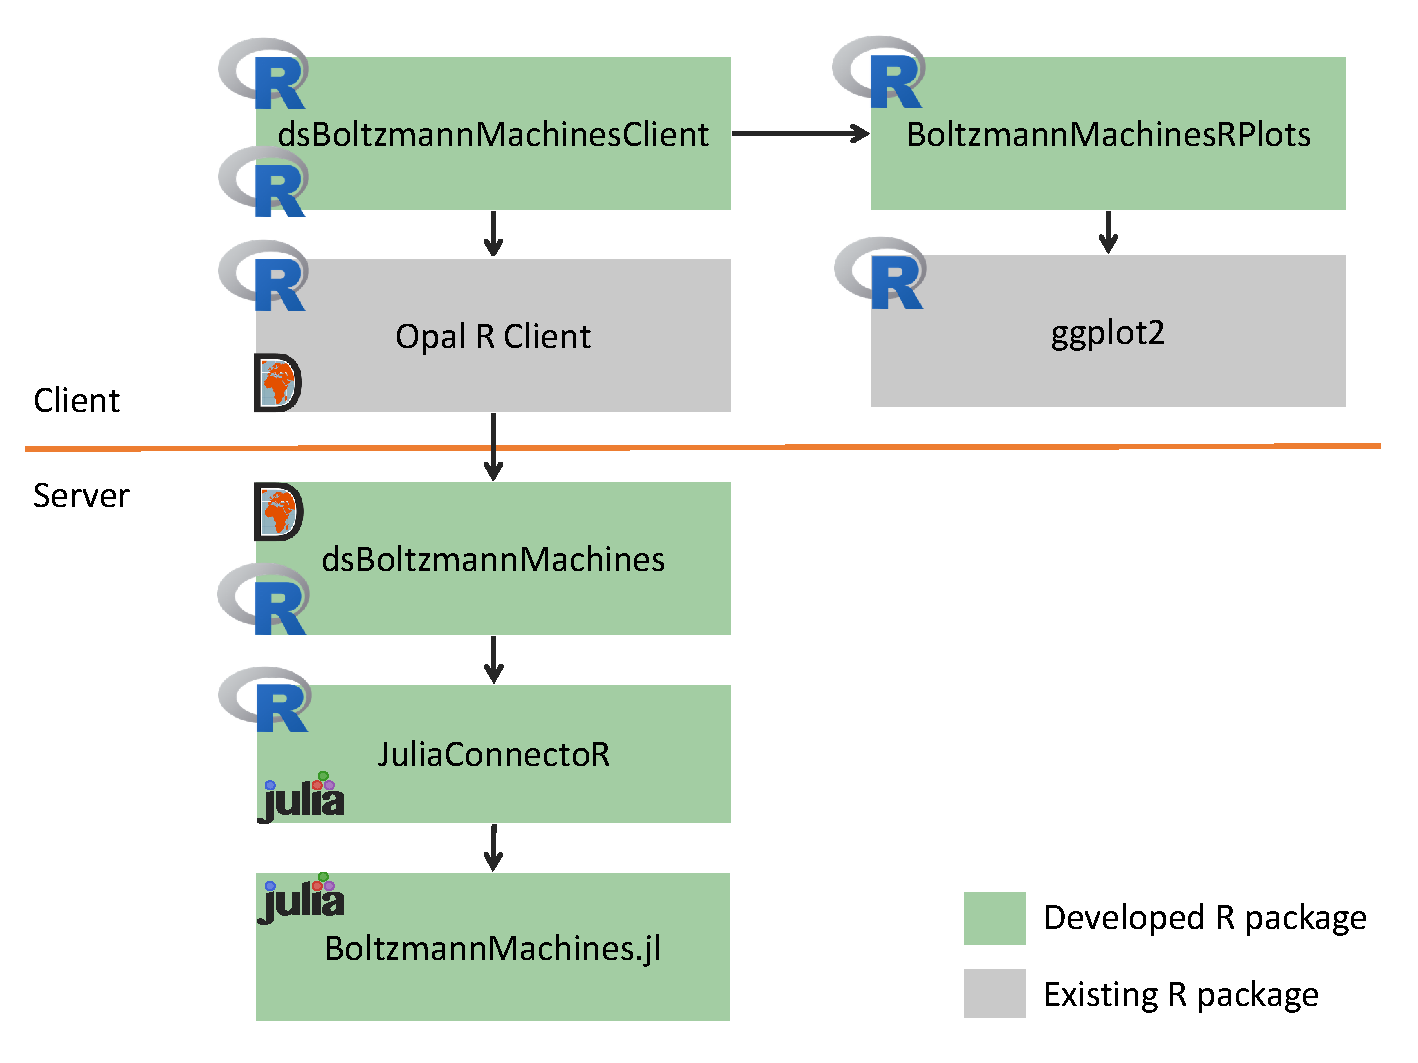
\includegraphics[scale=0.6]{images/dsBoltzmannMachinesOverview.pdf}
   \caption{Overview of the dependencies between the developed packages}
   \label{fig:dsBoltzmann_dependencies}
 \end{figure}   
 


In the following, the R code for performing the complete workflow as shown in Figure \ref{fig:examplaryworkflow} is detailed.
In a first step (see Listing \ref{lst:dslogin}), the user has to load the \apkg{dsBoltzmannMachinesClient} package and login to the remote Opal servers.
As the \apkg{dsBoltzmannMachinesClient} package depends on the Opal R client, that is loaded implicitly as well.
The login function can be used to obtain a DataSHIELD login object using the URL of the Opal server and the credentials of the user.
After a successful login, the resulting login object is assigned to the variable \inlinecode{o} here.
It is also possible to login to multiple Opal servers at once.
In this case the login object contains the references to multiple servers.
Calling functions via this login object sends the request parallely to multiple servers and  combines the results into one returned object. 
With the argument \inlinecode{assign} set to \inlinecode{TRUE}, the specified table is loaded and available by default as data set ``\inlinecode{D}'' on the server side.

\begin{lstlisting}[language=R,float=!h,caption={Loading package and logging in to the remote servers},label={lst:dslogin}]
library(dsBoltzmannMachinesClient)
logindata <- data.frame(server = "server",
                        url = "https://datashield.example.com",
                        user = "user", password = "password",
                        table = "MyTable")

o <- datashield.login(logins = logindata, assign = TRUE)
\end{lstlisting}

The created login object needs to be passed to the functions of the \apkg{dsBoltzmannMachinesClient} package to access the remote servers.
In a first step of the analysis, it is well advised to set a random seed to make the results of the stochastic algorithms reproducible.
The seed needs to be set in Julia because the random number generator of Julia is independent from that of R.

\begin{lstlisting}[language=R, float=!h]
ds.setJuliaSeed(o, 1)
\end{lstlisting}

The data set ``\inlinecode{D}'', which has been defined at the login above, can be split randomly into a training and a test data set.
These are assigned to the new variables \inlinecode{D.Train} and \inlinecode{D.Test} on the server side via the following call to \inlinecode{ds.splitdata}.
Here, 20\% of the data are used as test data.

\begin{lstlisting}[language=R, float=!h]
ds.splitdata(o, "D", 0.2, "D.Train", "D.Test")
\end{lstlisting}

A call to \inlinecode{ds.monitored\_fitdbm} fits a DBM on the training data.
The available arguments for the hyperparameters are the same as in the \apkg{BoltzmannMachines} Julia package.
Using both the training and the test data to evaluate the DBM may be used to determine the overfitting.
By default, the pre-training is monitored by evaluating the reconstruction error and the fine-tuning is monitored via estimating the lower bound of the log likelihood with AIS.
\begin{lstlisting}[language=R, float=!h]
result <- ds.monitored_fitdbm(o, data = "D.Train", 
                              nhiddens = c(50, 25, 15),
                              epochspretraining = 30,
                              learningratepretraining = 0.005,
                              epochs = 100,
                              learningrate = 0.05,
                              monitoringdata = c("D.Train",
                                                 "D.Test"))
\end{lstlisting}

The returned result contains by default only the monitoring information.
The trained model is assigned to a variable at the server side, which is called ``\inlinecode{dbm}'' by default.
(Subsequent functions that use a DBM will also assume this if it is not specified otherwise.)
It is technically possible to return the trained model itself, as the \apkg{JuliaConnectoR} can translate Julia objects to R objects, and the communication with the Opal server allows to return arbitrary R objects.
For increasing the data protection, returning the models is not allowed by default but it can be enabled by setting the variable \inlinecode{dsBoltzmannMachines.shareModels} to ``\inlinecode{TRUE}'' in the Opal server.
Technically this becomes possible because the \apkg{JuliaConnectoR} can translate complete Julia objects to R objects (see \ref{translatejuliar}).
Another option for data protection that can be set in the Opal server is the minimum number of samples that are required to train a model. This can be specified via the variable \inlinecode{dsBoltzmannMachines.privacyLevel}.

The \apkg{BoltzmannMachinesRPlots} package has implicitly been loaded as well when loading the \inlinecode{dsBoltzmannMachinesClient} package. 
With its \inlinecode{plotmonitoring} function, the learning curves \citep{ml_encyclopedia} can be displayed.
The resulting curves look similar to the ones shown in Figure \ref{fig:monitoring_bmplots}.

\begin{lstlisting}[language=R, float=!h]
plotMonitoring(result)
\end{lstlisting}

It is also possible to spare the monitoring by passing an empty vector as \inlinecode{monitoringdata} argument.
To get an impression of the amount of time that the training requires, Figure \ref{fig:dbmtrainingtimes} shows measurements taken with varying numbers of samples and variables.
The training time grows linearly with the number of samples if the hyperparameters are left unchanged.
If the number of variables is increased and the number of hidden nodes is scaled in the same proportion, the execution time grows quadratically.
These measurements show empirically what is expected theoretically, i.e., that the algorithm has the same time complexity as matrix multiplication.

\begin{figure}[hb]
   \centering
   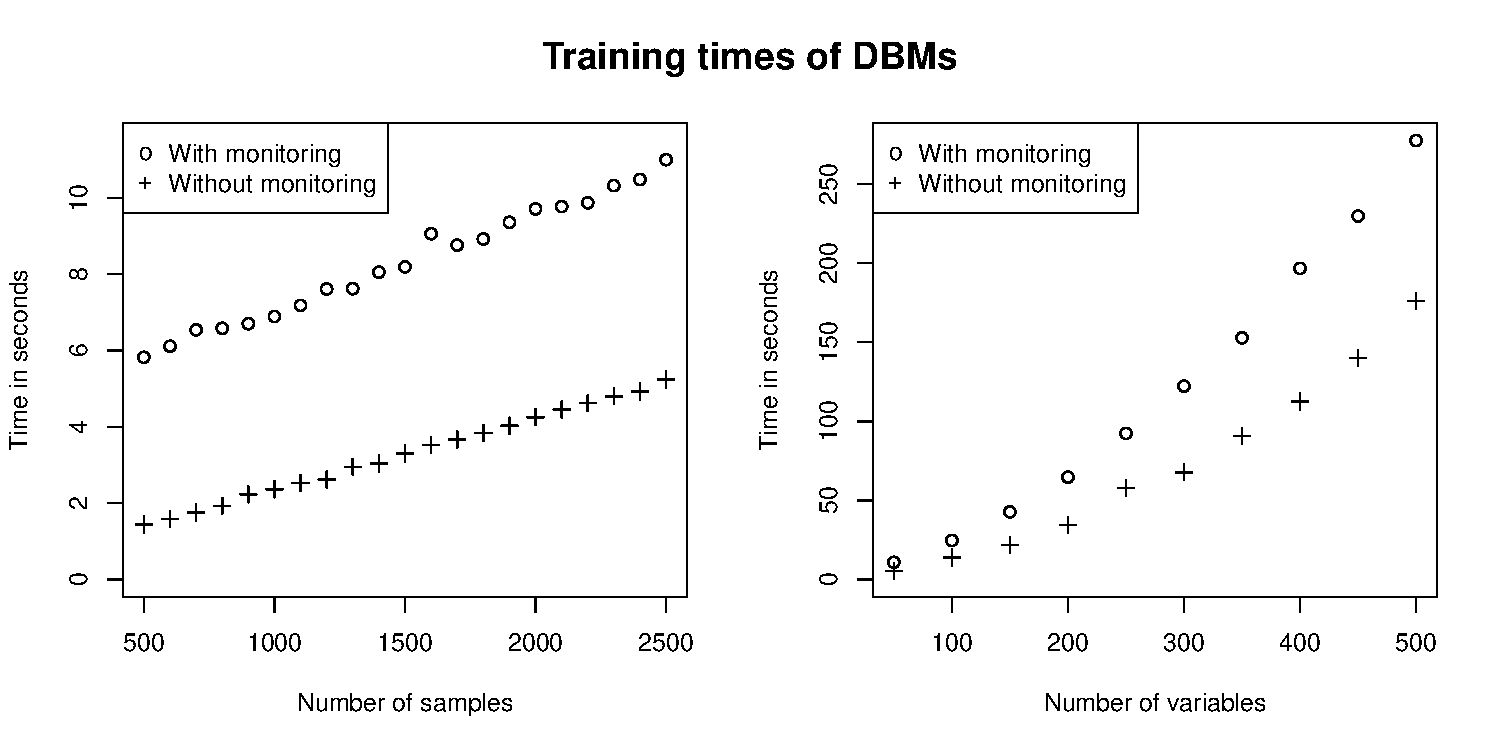
\includegraphics[scale=.6]{images/trainingtimes.pdf}
   \caption{Training duration of DBMs using the dsBoltzmannMachines package. On the left, the DBMs are trained on data sets with 50 variables and a varying number of samples. The DBMs have two hidden layers with 50 and 10 nodes, respectively. On the right, the number of samples is fixed as 2500. The DBMs are trained using data sets with varying numbers of variables. The hidden layers are scaled proportionally. In all cases the training consists of 30 epochs pre-training and 30 epochs fine-tuning and the monitoring is performed on the training data set and a test data set with 10 percent of the samples in the training data set. The times were measured on a virtual machine with one core, giving a lower bound of the performance. As can be seen, the performance scales in the same way as matrix multiplication. }
   \label{fig:dbmtrainingtimes}
 \end{figure}

Training without monitoring is faster but may give less insights about the choice of the hyperparameters (see \ref{monitoring}) because no learning curves can be shown.
Evaluating the training objective afterwards is still possible with the function \inlinecode{ds.dbm.logproblowerbound}.
When using this function it must be considered that the estimation is performed with a stochastic approximation algorithm and the results are therefore expected to differ slightly in different calls.

\begin{lstlisting}[language=R]
ds.dbm.logproblowerbound(o, data = "D.Train")
ds.dbm.logproblowerbound(o, data = "D.Test")
\end{lstlisting}



Most importantly, synthetic data can be generated by \inlinecode{ds.dbm.samples}. 

\begin{lstlisting}[language=R, float=!h]
generated <- ds.dbm.samples(o, nsamples = 1000)
\end{lstlisting}

It is also possible to perform a dimension reduction.
This can be done with the function \inlinecode{ds.dbm.top2LatentDims}, which performs a PCA on the logit-transformed mean-field activations that are induced by the data in the top hidden layer of the DBM.
An exemplary output can be seen in Figure \ref{fig:dbmvspca}.
\begin{lstlisting}[language=R]
ds.dbm.top2LatentDims(o, data = "D")
\end{lstlisting}

The resulting plot provides a clearly better dimension reduction than PCA alone in this case.
The five subgroups of the cases and the control group (see also Section \ref{simuexpsetup} for the textual description of the data set and Figure \ref{fig:distclustersnps}, panel A, for the hierarchical clustering view on the data set) form 6 distinct clusters there, which are not visible in the PCA.


 \begin{figure}[!hb]
   \centering
   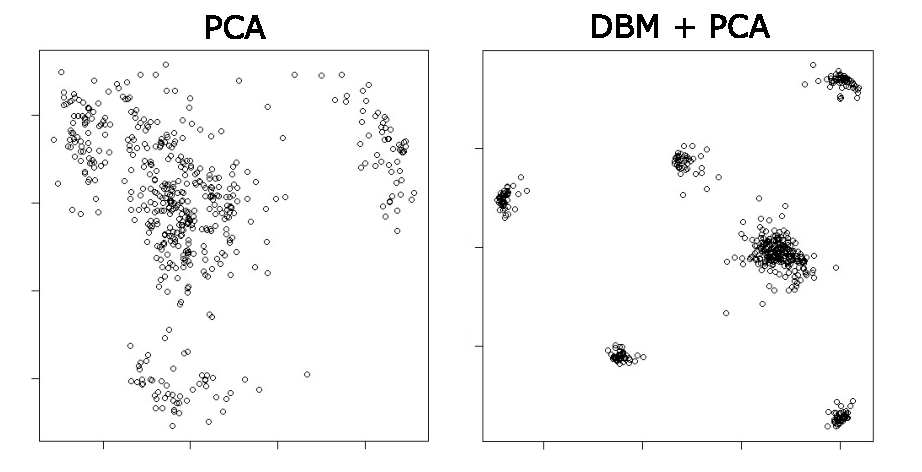
\includegraphics[scale=1]{images/dbmvspca.pdf}
   \caption{Dimension reduction using DBMs and PCA. The data set used is the simulated data set from Section \ref{simuexp}. Left: Principal component analysis (PCA) of the data. Right: Output from \inlinecode{ds.dbm.top2LatentDims}, which performs a PCA on  activation of the hidden nodes that is induced by the data using the mean-field algorithm.}
   \label{fig:dbmvspca}
 \end{figure}

In addition to DBMs, it is also possible to train RBMs and DBNs like in the \apkg{BoltzmannMachines} Julia package.
More complex partitioned architectures can be constructed as well by defining the parameters for individual layers via \inlinecode{ds.bm.defineLayer} and \inlinecode{ds.bm.definePartitionedLayer}.
Table \ref{tab:dsBoltzmannFuns} provides a summary of the available functions.
More detailed descriptions, including an explanation of the arguments, can be found in the documentation of the \apkg{dsBoltzmannMachinesClient} package, which is also reproduced in appendix \ref{dsbmsdoku}.

\rowcolors{1}{gray!25}{white}
\begin{table}[!htb]
\caption{Overview of the functions in the \apkg{dsBoltzmannMachinesClient} package}
\label{tab:dsBoltzmannFuns}
   \begin{tabularx}{\textwidth}{X}
   \Xhline{1pt}
\inlinecode{ds.monitored\_fitrbm} \rightpageref{rdokitem_ds.monitored.Rul.fitrbm} \\
Monitored training of an RBM model \\
\inlinecode{ds.monitored\_stackrbms} \rightpageref{rdokitem_ds.monitored.Rul.stackrbms} \\
Monitored training of a stack of RBMs. Can be used for pre-training a DBM or for training a DBN \\
\inlinecode{ds.monitored\_fitdbm} \rightpageref{rdokitem_ds.monitored.Rul.fitdbm} \\
Monitored training of a DBM, including pre-training and fine-tuning \\
\inlinecode{ds.setJuliaSeed} \rightpageref{rdokitem_ds.setJuliaSeed} \\
Set a seed for the random number generator \\
\inlinecode{ds.dbm.samples} / \inlinecode{ds.rbm.samples} \rightpagerefs{rdokitem_ds.dbm.samples}{rdokitem_ds.rbm.samples} \\
Generate samples from a DBM/RBM.
This also allows conditional sampling.\\
\inlinecode{ds.bm.defineLayer} \rightpageref{rdokitem_ds.bm.defineLayer} \\
Define training parameters individually for a RBM layer in a DBM or DBN \\
\inlinecode{ds.bm.definePartitionedLayer} \rightpageref{rdokitem_ds.bm.definePartitionedLayer} \\
Define a partitioned layer using other layers as parts \\
\inlinecode{ds.dbm.top2LatentDims} \rightpageref{rdokitem_ds.dbm.top2LatentDims} \\
Get a two-dimensional representation of latent features \\
\inlinecode{ds.rbm.loglikelihood} \rightpageref{rdokitem_ds.rbm.loglikelihood} \\
Estimates the partition function of an RBM with AIS and then calculates the log-likelihood \\
\inlinecode{ds.dbm.loglikelihood} \rightpageref{rdokitem_ds.dbm.loglikelihood} \\
Performs a separate AIS run for each of the samples to estimate the log-likelihood of a DBM \\
\inlinecode{ds.dbm.logproblowerbound} \rightpageref{rdokitem_ds.dbm.logproblowerbound} \\
Estimates the variational lower bound of the likelihood of a DBM with AIS \\
\inlinecode{ds.rbm.exactloglikelihood} /
\inlinecode{ds.dbm.exactloglikelihood} \rightpagerefs{rdokitem_ds.dbm.exactloglikelihood}{rdokitem_ds.rbm.exactloglikelihood} \\
Calculates the log-likelihood for a RBM/DBM (exponential complexity)\\
   \Xhline{1pt}
\end{tabularx}
\end{table}

%\begin{figure}[h]
%   \centering
%   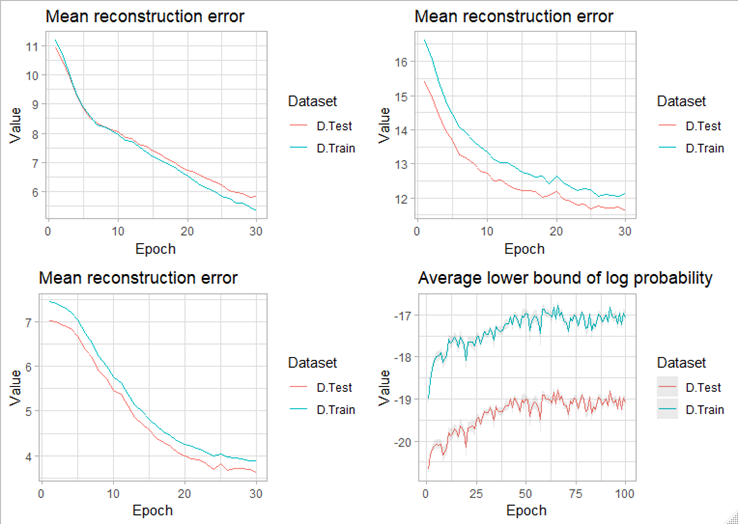
\includegraphics[scale=0.4,trim={0.1cm 0 0 0.1cm},clip]{images/dsBoltzmannLearningcurves.png}
%   \caption{Examples for learning curves produced by the package \apkg{BoltzmannMachinesPlots}. This shows learning curves for the training of a DBM with three layers. The plots showing the mean reconstruction error are the result of monitoring the greedy layerwise pre-training. The plot showing the lower bound of the log probability comes is the monitoring output of the fine-tuning of the DBM. There are two curves in each plot, one for the training data and one for the test data.}
% \end{figure}


\clearpage
\FloatBarrier

\section{Discussion}

\subsection{Computational performance}
For performing deep learning on large quantities of image and text data, the need for special hardware rises \citep{lecun_dlhardware}.
Major breakthroughs in language processing and image recognition such as the famous models {\em GPT-3} and \citep{gpt3} {\em ResNet} \citep{resnet} build on very deep architectures with many parameters.
This may give the impression that immense amounts of data and computation are needed to make use of deep learning at all.
The results of the experiments conducted here (see \ref{simuexpresults} and \ref{realexpresults}) show that deep learning can bring also benefits on a smaller scale, particularly in settings with lower sample sizes.
With the software employed here, the speed of the training was sufficient, even utilizing only standard hardware.
This demonstrates that deep learning can also be feasible and beneficial without investments in dedicated hardware.

But, of course, performance improvements are worth considering.
When optimizing software solutions, it must, however, always be taken into account that such changes cost time when implementing them, and they may cost additional time in the future if the flexibility to apply further changes is affected by the optimization.
This dilemma has been addressed in the famous quote "premature optimization is the root of all evil" \citep{knuth_1974}.
The dilemma exists also in research software development because the resulting software needs to be subject to experimentation.

Julia was chosen as language for the implementation of deep Boltzmann machines here because it aims to hit the sweet spot in this dilemma with its attempt to solve the ``two-language problem'' \citep{bezanson2017julia}, i.e., having one scripting language, such as Python, for fast development and prototyping, and an additional low-level language, such as C or Fortran, for speeding up time-critical parts.
With Julia aiming at the speed of C, there is no need to move parts of the implementation to a low-level language.
Improvements such as reusing allocated space (see \ref{impltechnology} for more details) can be implemented directly in Julia.

Optimizing the performance of the implementation of deep Boltzmann machines could be done via further parallelizing the algorithms.
With their special architecture, graphics processing units (GPUs) allow a massive parallelization of operations that are executed simultaneously in the same way on different data points.
Many deep learning frameworks such as \apkg{TensorFlow} \citep{tensorflow} and \apkg{PyTorch} \citep{pytorch} support to run code on GPUs in addition to the central processing unit (CPU).
Also the Julia package \apkg{Flux} supports to run array operations on NVIDIA GPUs via the \apkg{CUDA} Julia package \citep{juliagpu}.
As the multiplication of large matrices is already multi-threaded on CPUs with multiple cores, performance gains by moving computations to the GPU may only be expected if the matrix operations exhaust the threading capabilities of the CPU.
On CPUs with multiple cores, multi-threading can speed up the matrix multiplications for large matrices.
This is done by the highly optimized OpenBLAS library, which is employed by Julia and which is capable of multi-threading internally \citep{openblas}.
To get substantial performance improvements by switching to GPU computing, the matrices need to have a sufficient size \citep{performancegpucpu}.
This size is restricted by the batch size, as the update in the training algorithm can only be parallelized for samples in the same batch, and large batch sizes are not desirable in all cases \citep{masters_revisiting_2018}.
Moreover, specific hardware requirements such as restrictions to certain types of graphics cards of a specific vendor make this kind of optimizations less attractive, in particular when considering a distributed setting, such as discussed in Section \ref{deepgends}, involving several clinics with different compute infrastructures.
Given these considerations, which show that it is not trivial to harness the power of GPUs, a definitive use case where the performance would be needed to investigate this direction further.


\subsection{Generative performance and modeling capabilities}
The experiment shown in Section \ref{realexp} builds on \cite{nussberger_synthetic_2020} where the generative performance of DBMs, VAEs, and GANs is compared in diverse settings, in particular with a broad range regarding the number of samples.
The results of \cite{nussberger_synthetic_2020} show that DBMs and VAEs are suitable as generative models for genetic variant data, while the generative performance GANs is insufficient in settings of low sample size.
Here, these approaches are investigated in settings where data is distributed across a number of sites.
The results for the generative performance in these distributed settings are in concordance with \cite{nussberger_synthetic_2020}.

The comparison to the MICE model, which has been used as an approach for creating synthetic data in practice \citep{mice_buuren_2011}, shows that applying deep learning can lead to clearly superior results also in small data sets.
It also shows that not all deep learning models are suited well for such settings and the size of the data set is a factor to consider when choosing a deep learning approach.

The networks considered in the experiments were densely connected. 
For modeling higher dimensional data, more parsimonious models may perform better \citep{nussberger_synthetic_2020}.
More generally, saving parameters can aid in training models also with fewer data points per dimension \citep{chan_classifier_1999}.
One approach for reducing the number of parameters in DBMs is to partition the layers.
For genetic variant data, an approach using sparse regression for partitioning clusters of SNPs has been examined in DBMs \citep{hess2017partitioned} and lead to meaningful results.
The implementation was also based on the \apkg{BoltzmannMachines} package.
The concept of multimodal DBMs in the package allows to train DBMs with partitioned layers conveniently.
It is based on using restricted Boltzmann machines (RBMs) as building blocks.
This makes it also easy to model different distributions at the visible layer.
\cite{treppner_making_2020} used this feature to construct DBMs with input variables following negative binomial distributions for clustering single-cell sequencing data.

\subsection{Disclosure risk of synthetic data}
In addition to evaluating the performance, the disclosure risk is regarded here as well, with a focus on membership disclosure \citep{li_membership_2013}.
For this, a new approach to evaluate the disclosure risk by assessing the overfitting via the proposed ``proportion of overfitting'' (see \ref{proportionoverfitting}).
As an additional method for measuring the disclosure risk, simulated membership attacks are performed \citep{goncalves}.
Both disclosure metrics can be applied directly to the synthetic data without having to distort the data or having to modify the training to control the disclosure, as it is needed when applying differential privacy \citep{dwork_differential_2008, abadi_deep_2016}.

The membership attack requires to take the sensitivity and the attackers' distance threshold  into account when interpreting the precision.
The advantage of the proportion of overfitting is that it consists of a single number.
It can therefore be used more easily to compare two models directly with respect to disclosure.
The proportion of overfitting has also an intuitive meaning.
It is the amount of which a model learns more about the training data than about the general structure of the underlying data distribution.

In both the results of the proportion of overfitting and the precision of the membership attacks, DBMs and VAEs do not exhibit an increased disclosure risk compared to the simpler approaches IM and MICE.
Particularly interesting is the higher variance in the precision of the membership attack on MICE compared to VAEs and DBMs.
One can interpret this as a higher disclosure risk of MICE compared to the two neural network approaches in this scenario.
This means that there is not more identifying information derivable from the synthetic data generated by a DBM or VAE than from data generated via a sequence of logistic regression models, such as in the MICE method.
This is in contrast to the possible intuition that the more complex approaches must have a higher risk of leaking information.
Since DataSHIELD allows to extract information via logistic regression models and it is therefore possible to use the MICE method to generate synthetic data from the DataSHIELD client side already, one can argue that using DBMs or VAEs as generative approaches does not lower the level of privacy in a setting where DataSHIELD is used.

In DataSHIELD only known users are allowed to conduct analyses and their activity is logged to prevent analyses with malicious intent.
If data is to be released completely without restrictions, e.g., by putting it on a internet site for anyone to download and analyze, the privacy concerns are higher than in a setting where only known users analyze data via DataSHIELD.
In an unrestricted scenario, additional measures are needed to ensure the best confidence in the protection of sensitive data.
Yet, this applies regardless of the data protection method, as all approaches for managing the disclosure risk work with thresholds, which are hard to validate and also cannot give an absolute certainty (see \ref{privacyconcepts}).
A combination of different disclosure metrics and human assessment can minimize the risk in such cases.

Summed up, the results strengthen the assumption that it is possible to use DBMs, and additionally VAEs, for generating synthetic data from sensitive data of individuals.


%\subsection{Handling different data types}
%one step for applying arbitrary tabular data.

%dbms verbessern missing values, softmax evaluieren
%TODO martin paper zitieren?
%Privacy-consideration better use intensity values.


\subsection{Outlook}

\cite{hinton_reducing_2006} used deep belief networks to pre-train autoencoder networks, which were then fine-tuned using backpropagation.
This was done to overcome the problem that the backpropagation algorithm alone was not able to find a good solution given a limited amount of data \citep{lecun_deep_learning_2015}.
It might be interesting to investigate whether {\em variational} autoencoders could profit in the same way from such a pre-training in settings of low sample size, as they are also trained via backpropagation. 

Another idea to create better synthetic data sets could be to combine different types of generative models in ensembles of generative models.
Ensemble learning is mostly done with classification tasks \citep{ensemble_learning_survey_2018}.
Ensembles of predictive models are used to increase the predictive performance.
Multiple models are trained on the data and their predictions are combined to get a better predictor.
Unsupervised ensembles have been used for outlier detection \citep{unsupervised_outlier}.
The heterogeneity between the models can prevent overfitting and thereby leads to results that generalize better \citep{ensemble_learning_survey_2018}.
Translating this idea to increase the quality of synthetic data could therefore be promising, in particularly in setting of small sample size, where the issue of overfitting is most important.
Using generative ensembles has been investigated in GANs to prevent mode collapse and increase the diversity of generated samples \citep{toutouh_ensemblegan_2020}.
For creating synthetic data, multiple models can be used to enhance the performance with respect to a performance criterion that is applied on combined data from different models.
Experimentally this could be investigated with a similar setup to the one in the distributed experiments.
In the experiments with simulated and real genetic variant data here, the data is split in different parts, corresponding to different sites/clinics.
Synthetic data is generated from different models that have been trained on different parts. Then, the resulting synthetic data sets are combined and evaluated.
A very similar approach can be used to investigate generative ensembles. 
Instead of splitting the data, the same data but different generative approaches can be used to create the parts of the synthetic data set.
The combined synthetic data can be assessed in a similar way as shown here with respect to performance and disclosure.
This way, the question whether a combination of different approaches can lead to better and more diverse synthetic data could be studied further.

The findings here indicate that DBMs and VAEs can both be suitable for data of small sample size.
Combining their generative capabilities could therefore be particularly promising.
A first step could be to implement VAEs in DataSHIELD as an additional deep generative approach.
This can be done analogously to the implementation shown in Section \ref{dsBoltzmannMachinesImpl}.
VAEs can be constructed and trained using the \apkg{Flux} package in Julia.
The interface can be wrapped in a DataSHIELD R package via the \apkg{JuliaConnectoR}.
The same approach can be taken for all kinds of other generative models.
Using an example of neural differential equations models \citep{juliaconnector_2021, chen_neural_2019}, it has been demonstrated that also complex neural networks based on \apkg{Flux} can be wrapped via the \apkg{JuliaConnectoR} for being handled in R.
This shows that it is in principle possible to bring very diverse deep learning algorithms into the DataSHIELD infrastructure.

\subsection{Conclusion}
Deep learning can help to create synthetic data that preserve higher-level structures in biomedical data.
Both DBMs and VAEs are promising models for creating synthetic data from data of small sample size, whereas GANs do not perform well in such settings.
Even given only a limited number of samples, DBMs and VAEs can generate clearly better synthetic data than simpler methods such as multiple imputation via chained logistic regression models.
Using deep learning for generating synthetic data from sensitive information such as genetic variant data of individuals does not necessarily result in an increased disclosure risk.

The implementation of DBMs in Julia via the \apkg{BoltzmannMachines} package allows a flexible composition of DBMs from building blocks of RBMs.
It also offers convenient methods for evaluating the training.
This is important for finding good hyperparameters, which is especially relevant when regarding the diversity of biomedical data sets, where default values for hyperparameters are often not sufficient.

Algorithms and data structures from Julia can be accessed in R via the \apkg{JuliaConnectoR} R package.
This allows wrapping the functionality of the \apkg{BoltzmannMachines} package into a DataSHIELD R package.
With the same mechanism, VAEs or other complex generative models could be integrated in DataSHIELD for enabling distributed analyses based on synthetic data.

\clearpage
\appendix



\begin{appendices}
\singlespacing
\section{References}

\renewcommand{\bibsection}{} % funzt nur mit natbib: https://tex.stackexchange.com/a/370784/206178

\bibliography{references}

\clearpage
\onehalfspacing
\section[Publications and declaration of own contributions]{Publications and declaration of \\ own contributions}
Parts of this work have been published in the following articles:

\begin{enumerate}[(1)]
\item
Lenz, S., Hess, M. \harvardand\ Binder, H.  \harvardyearleft
   2019\harvardyearright , `Unsupervised deep learning on biomedical data with \apkg{BoltzmannMachines.jl}', {\em bioRxiv 578252}.
\newline\harvardurl{\url{https://doi.org/10.1101/578252}}

\item 
Lenz, S., Hackenberg, M. \harvardand\ Binder, H.  \harvardyearleft
  2021\harvardyearright , `The {JuliaConnectoR}: a functionally oriented
  interface for integrating {Julia} in {R}', {\em arXiv:2005.06334 [cs, stat]}. 
  \newline(Accepted by the {\em Journal of Statistical Software})
\newline\harvardurl{\url{http://arxiv.org/abs/2005.06334}}

\item
Lenz, S., Hess, M. \harvardand\ Binder, H.  \harvardyearleft
  2021\harvardyearright , `Deep generative models in {DataSHIELD}', {\em BMC
  Medical Research Methodology} {\bf 21}(1),~64.
\newline\harvardurl{\url{https://doi.org/10.1186/s12874-021-01237-6}}
\end{enumerate}

All three articles have been written primarily by me under the supervision of Prof.~Dr.~Harald Binder. 
All plots and drawings have been created by myself.
All artwork that was used for composing the drawings does not require attribution.
The contributions to the publications and to the underlying software packages are further:

\begin{enumerate}[(1)]
\item
Harald Binder contributed to the initial design of the \apkg{BoltzmannMachines} package by creating a Julia version from a MATLAB predecessor that I wrote.
I then developed the Julia code further and made the training more flexible, added the concept of multimodal DBMs, and put a special emphasis for evaluating the training.
Moritz Hess contributed by providing the perspective of the application on omics data.

\item
I devised the design of the \apkg{JuliaConnectoR} package and implemented it.
Harald Binder contributed by requesting features for convenient interactive use, thereby steering the software design into this direction.
Maren Hackenberg contributed the example for using neural differential equations in the article. 
This example is not included in the thesis.

\item
I developed the concept for the analysis and the simulation design with the advice of Harald Binder. I designed and implemented the software and conducted the analyses. Moritz Hess contributed to  the experiment for comparing the different generative models on genetic variant data by preparing the data and giving advice for the model training.
\end{enumerate}




\setlength{\emergencystretch}{3em}

\clearpage
\section[Documentation of Julia package \apkg{BoltzmannMachines}]{Documentation of Julia package \\ \apkg{BoltzmannMachines}}
\label{BMDoku}

This appendix lists the documentation for all exported and documented items of the \apkg{BoltzmannMachines} Julia package, as of version 1.2.0. The code of the package and more documentation can be found on the GitHub repository \url{https://github.com/stefan-m-lenz/BoltzmannMachines.jl}.

\subsection*{AbstractOptimizer}
The \texttt{AbstractOptimizer} interface allows to specify optimization procedures. It consists of three methods:

\begin{itemize}
\item \texttt{initialized(optimizer, bm)}: May be used for creating an optimizer that is  specifically initialized for the Boltzmann machine \texttt{bm}.  In particular it may be used to allocate reusable space for the gradient.  The default implementation simply returns the unmodified \texttt{optimizer}.


\item \texttt{computegradient!(optimizer, v, vmodel, h, hmodel, rbm)} or \texttt{computegradient!(optimizer, meanfieldparticles, gibbsparticles, dbm)}  needs to be implemented for computing the gradient given the samples  from the positive and negative phase.


\item \texttt{updateparameters!(bm, optimizer)} needs to be specified for taking the  gradient step. The default implementation for RBMs expects the fields  \texttt{learningrate} and \texttt{gradient} and adds \texttt{learningrate * gradient} to the  given RBM.

\end{itemize}
\noindent\rule{\textwidth}{1pt}
%======================================================
\subsection*{AbstractRBM}
Abstract supertype for all RBMs 

\noindent\rule{\textwidth}{1pt}
%======================================================
\subsection*{AbstractTrainLayer}
Abstract supertype for layerwise training specification. May be specifications for a normal RBM layer (see \texttt{TrainLayer}) or multiple combined specifications for a partitioned layer (see \texttt{TrainPartitionedLayer}).

\noindent\rule{\textwidth}{1pt}
%======================================================
\subsection*{BernoulliGaussianRBM}
\begin{verbatim}
BernoulliGaussianRBM(weights, visbias, hidbias)
\end{verbatim}
Encapsulates the parameters of an RBM with Bernoulli distributed visible nodes and Gaussian distributed hidden nodes. The standard deviation of the Gaussian distribution is 1.

\noindent\rule{\textwidth}{1pt}
%======================================================
\subsection*{BernoulliRBM}
\begin{verbatim}
BernoulliRBM(weights, visbias, hidbias)
\end{verbatim}
Encapsulates the parameters of an RBM with Bernoulli distributed nodes.

\begin{itemize}
\item \texttt{weights}: matrix of weights with size (number of visible nodes, number of hidden nodes)


\item \texttt{visbias}: bias vector for visible nodes


\item \texttt{hidbias}: bias vector for hidden nodes

\end{itemize}
\noindent\rule{\textwidth}{1pt}
%======================================================
\subsection*{Binomial2BernoulliRBM}
\begin{verbatim}
Binomial2BernoulliRBM(weights, visbias, hidbias)
\end{verbatim}
Encapsulates the parameters of an RBM with 0/1/2-valued, Binomial (n=2) distributed visible nodes, and Bernoulli distributed hidden nodes. This model is equivalent to a BernoulliRBM in which every two visible nodes are connected with the same weights to each hidden node. The states (0,0) / (1,0) / (0,1) / (1,1) of the visible nodes connected with with the same weights translate as states 0 / 1 / 1 / 2 in the Binomial2BernoulliRBM.

\noindent\rule{\textwidth}{1pt}
%======================================================
\subsection*{DataDict}
A dictionary containing names of data sets as keys and the data sets (matrices with samples in rows) as values.

\noindent\rule{\textwidth}{1pt}
%======================================================
\subsection*{GaussianBernoulliRBM}
\begin{verbatim}
GaussianBernoulliRBM(weights, visbias, hidbias, sd)
\end{verbatim}
Encapsulates the parameters of an RBM with Gaussian distributed visible nodes and Bernoulli distributed hidden nodes.

\noindent\rule{\textwidth}{1pt}
%======================================================
\subsection*{GaussianBernoulliRBM2}
\begin{verbatim}
GaussianBernoulliRBM2(weights, visbias, hidbias, sd)
\end{verbatim}
Encapsulates the parameters of an RBM with Gaussian distributed visible nodes and Bernoulli distributed hidden nodes with the alternative energy formula proposed by KyungHyun Cho.

\noindent\rule{\textwidth}{1pt}
%======================================================
\subsection*{LoglikelihoodOptimizer}
Implements the \texttt{AbstractOptimizer} interface for optimizing the loglikelihood with stochastic gradient descent.

\noindent\rule{\textwidth}{1pt}
%======================================================
\subsection*{Monitor}
A vector for collecting \texttt{MonitoringItem}s during training.

\noindent\rule{\textwidth}{1pt}
%======================================================
\subsection*{MonitoringItem}
Encapsulates the value of an evaluation calculated in one training epoch. If the evaluation depends on a dataset, the dataset's name can be specified also.

\noindent\rule{\textwidth}{1pt}
%======================================================
\subsection*{Particles}
\texttt{Particles} are an array of matrices. The i'th matrix contains in each row the vector of states of the nodes of the i'th layer of an RBM or a DBM. The set of rows with the same index define an activation state in a Boltzmann Machine. Therefore, the size of the i'th matrix is (number of samples/particles, number of nodes in layer i).

\noindent\rule{\textwidth}{1pt}
%======================================================
\subsection*{PartitionedRBM}
\begin{verbatim}
PartitionedRBM(rbms)
\end{verbatim}
Encapsulates several (parallel) AbstractRBMs that form one partitioned RBM. The nodes of the parallel RBMs are not connected between the RBMs.

\noindent\rule{\textwidth}{1pt}
%======================================================
\subsection*{TrainLayer}
Specify parameters for training one RBM-layer in a DBM.

\paragraph*{Optional keyword arguments:}
\begin{itemize}
\item The optional keyword arguments \texttt{rbmtype}, \texttt{nhidden}, \texttt{epochs}, \texttt{learningrate}/\texttt{learningrates}, \texttt{sdlearningrate}/\texttt{sdlearningrates}, \texttt{categories}, \texttt{batchsize}, \texttt{pcd}, \texttt{cdsteps}, \texttt{startrbm} and \texttt{optimizer}/\texttt{optimizers} are passed to \texttt{fitrbm}. For a detailed description, see there. If a negative value is specified for \texttt{learningrate} or \texttt{epochs}, this indicates that a corresponding default value should be used (parameter defined by call to \texttt{stackrbms}).


\item \texttt{monitoring}: also like in \texttt{fitrbm}, but may take a \texttt{DataDict} as third argument  (see function \texttt{stackrbms} and its argument \texttt{monitoringdata}).


\item \texttt{nvisible}: Number of visible units in the RBM. Only relevant for partitioning.  This parameter is derived as much as possible by \texttt{stackrbms}.  For \texttt{MultimodalDBM}s with a partitioned first layer, it is necessary to specify  the number of visible nodes for all but at most one partition in the input layer.

\end{itemize}
\noindent\rule{\textwidth}{1pt}
%======================================================
\subsection*{TrainPartitionedLayer}
Encapsulates a vector of \texttt{TrainLayer} objects for training a partitioned layer.

\noindent\rule{\textwidth}{1pt}
%======================================================
\subsection*{aislogimpweights}
\begin{verbatim}
aislogimpweights(rbm; ...)
\end{verbatim}
Computes the logarithmised importance weights for estimating the ratio of the partition functions of the given \texttt{rbm} to the RBM with zero weights, but same visible and hidden bias as the \texttt{rbm}. This function implements the Annealed Importance Sampling algorithm (AIS) like described in section 4.1.3 of [Salakhutdinov, 2008].

\paragraph*{Optional keyword arguments (for all types of Boltzmann Machines):}
\begin{itemize}
\item \texttt{ntemperatures}: Number of temperatures for annealing from the starting model to the target model, defaults to 100


\item \texttt{temperatures}: Vector of temperatures. By default \texttt{ntemperatures} ascending numbers, equally spaced from 0.0 to 1.0


\item \texttt{nparticles}: Number of parallel chains and calculated weights, defaults to  100


\item \texttt{burnin}: Number of steps to sample for the Gibbs transition between models

\end{itemize}
\begin{verbatim}
aislogimpweights(rbm1, rbm2; ...)
\end{verbatim}
Computes the logarithmised importance weights for estimating the log-ratio log(Z2/Z1) for the partition functions Z1 and Z2 of \texttt{rbm1} and \texttt{rbm2}, respectively. Implements the procedure described in section 4.1.2 of [Salakhutdinov, 2008]. This requires that \texttt{rbm1} and \texttt{rbm2} are of the same type and have the same number of visible units.

\begin{verbatim}
aislogimpweights(dbm; ...)
\end{verbatim}
Computes the logarithmised importance weights in the Annealed Importance Sampling algorithm (AIS) for estimating the ratio of the partition functions of the given DBM \texttt{dbm} to the base-rate DBM with all weights being zero and all biases equal to the biases of the \texttt{dbm}.

Implements algorithm 4 in [Salakhutdinov+Hinton, 2012]. For DBMs with Bernoulli-distributed nodes only (i. e. here DBMs of type \texttt{PartitionedBernoulliDBM}), it is possible to calculate the importance weights by summing out either the even layers (h1, h3, ...) or the odd layers (v, h2, h4, ...). In the first case, the nodes' activations in the odd layers are used to calculate the probability ratios, in the second case the even layer are used. If \texttt{dbm} is of type \texttt{PartitionedBernoulliDBM}, the optional keyword argument \texttt{sumout} can be used to choose by specifying the values \texttt{:odd} (default) or \texttt{:even}. In the case of \texttt{MultimodalDBM}s, it is not possible to choose and the second case applies there.

\noindent\rule{\textwidth}{1pt}
%======================================================
\subsection*{aisprecision}
\begin{verbatim}
aisprecision(logr, aissd, sdrange)
\end{verbatim}
Returns the differences of the estimated logratio \texttt{r} to the lower and upper bound of the range defined by the multiple \texttt{sdrange} of the standard deviation of the ratio's estimator \texttt{aissd}.

\begin{verbatim}
aisprecision(logimpweights, sdrange)
\end{verbatim}
\noindent\rule{\textwidth}{1pt}
%======================================================
\subsection*{aisstandarddeviation}
Computes the standard deviation of the AIS estimator (not logarithmised) (eq 4.10 in [Salakhutdinov+Hinton, 2012]) given the logarithmised importance weights.

\noindent\rule{\textwidth}{1pt}
%======================================================
\subsection*{barsandstripes}
\begin{verbatim}
barsandstripes(nsamples, nvariables)
\end{verbatim}
Generates a test data set. To see the structure in the data set, run e. g. \texttt{reshape(barsandstripes(1, 16), 4, 4)} a few times.

Example from: MacKay, D. (2003). Information Theory, Inference, and Learning Algorithms

\noindent\rule{\textwidth}{1pt}
%======================================================
\subsection*{computegradient!}
\begin{verbatim}
computegradient!(optimizer, v, vmodel, h, hmodel, rbm)
\end{verbatim}
Computes the gradient of the RBM \texttt{rbm} given the the hidden activation \texttt{h} induced by the sample \texttt{v} and the vectors \texttt{vmodel} and \texttt{hmodel} generated by sampling from the model. The result is stored in the \texttt{optimizer} in such a way that it can be applied by a call to \texttt{updateparameters!}. There is no return value.

For RBMs (excluding PartitionedRBMs), this means saving the gradient in a RBM of the same type in the field \texttt{optimizer.gradient}.

\noindent\rule{\textwidth}{1pt}
%======================================================
\subsection*{crossvalidation}
\begin{verbatim}
crossvalidation(x, monitoredfit; ...)
\end{verbatim}
Performs k-fold cross-validation, given

\begin{itemize}
\item the data set \texttt{x} and


\item \texttt{monitoredfit}: a function that fits and evaluates a model. As arguments it must accept:

\begin{itemize}
\item a training data data set


\item a \texttt{DataDict} containing the evaluation data.

\end{itemize}
\end{itemize}
The return values of the calls to the \texttt{monitoredfit} function are concatenated with \texttt{vcat}. If the monitoredfit function returns \texttt{Monitor} objects, \texttt{crossvalidation} returns a combined \texttt{Monitor} object that can be displayed by creating a cross-validation plot via \texttt{BoltzmannMachinesPlots.crossvalidationplot}.

\paragraph*{Optional named argument:}
\begin{itemize}
\item \texttt{kfold}: specifies the \texttt{k} in "\texttt{k}-fold" (defaults to 10).

crossvalidation(x, monitoredfit, pars; ...)

\end{itemize}
If additionaly a vector of parameters \texttt{pars} is given, \texttt{monitoredfit} also expects an additional parameter from the parameter set.

\noindent\rule{\textwidth}{1pt}
%======================================================
\subsection*{empiricalloglikelihood}
\begin{verbatim}
empiricalloglikelihood(x, xgen)
empiricalloglikelihood(bm, x, nparticles)
empiricalloglikelihood(bm, x, nparticles, burnin)
\end{verbatim}
Computes the mean empirical loglikelihood for the data set \texttt{x}. The probability of a sample is estimated to be the empirical probability of the sample in a dataset generated by the model. This data set can be given as \texttt{xgen} or it is generated by running a Gibbs sampler with \texttt{nparticles} for \texttt{burnin} steps (default 5) in the Boltzmann Machine \texttt{bm}. Throws an error if a sample in \texttt{x} is not contained in the generated data set.

\noindent\rule{\textwidth}{1pt}
%======================================================
\subsection*{energy}
\begin{verbatim}
energy(rbm, v, h)
\end{verbatim}
Computes the energy of the configuration of the visible nodes \texttt{v} and the hidden nodes \texttt{h}, specified as vectors, in the \texttt{rbm}.

\noindent\rule{\textwidth}{1pt}
%======================================================
\subsection*{exactloglikelihood}
\begin{verbatim}
exactloglikelihood(rbm, x)
\end{verbatim}
Computes the mean log-likelihood for the given dataset \texttt{x} and the RBM \texttt{rbm} exactly. The log of the partition function is computed exactly by \texttt{exactlogpartitionfunction(rbm)}. Besides that, the function simply calls \texttt{loglikelihood(rbm, x)}.

\begin{verbatim}
exactloglikelihood(dbm, x)
exactloglikelihood(dbm, x, logz)
\end{verbatim}
Computes the mean log-likelihood for the given dataset \texttt{x} and the DBM \texttt{dbm} exactly. If the value of the log of the partition function of the \texttt{dbm} is not supplied as argument \texttt{logz}, it will be computed by \texttt{exactlogpartitionfunction(dbm)}.

\noindent\rule{\textwidth}{1pt}
%======================================================
\subsection*{exactlogpartitionfunction}
\begin{verbatim}
exactlogpartitionfunction(rbm)
\end{verbatim}
Calculates the log of the partition function of the BernoulliRBM \texttt{rbm} exactly. The execution time grows exponentially with the minimum of (number of visible nodes, number of hidden nodes).

\begin{verbatim}
exactlogpartitionfunction(gbrbm)
\end{verbatim}
Calculates the log of the partition function of the GaussianBernoulliRBM \texttt{gbrbm} exactly. The execution time grows exponentially with the number of hidden nodes.

\begin{verbatim}
exactlogpartitionfunction(bgrbm)
\end{verbatim}
Calculates the log of the partition function of the BernoulliGaussianRBM \texttt{bgrbm} exactly. The execution time grows exponentially with the number of visible nodes.

\begin{verbatim}
exactlogpartitionfunction(dbm)
\end{verbatim}
Calculates the log of the partition function of the DBM \texttt{dbm} exactly. If the number of hidden layers is even, the execution time grows exponentially with the total number of nodes in hidden layers with odd indexes (i. e. h1, h3, ...). If the number of hidden layers is odd, the execution time grows exponentially with the minimum of (number of nodes in layers with even index, number of nodes in layers with odd index).

\begin{verbatim}
exactlogpartitionfunction(mdbm)
\end{verbatim}
Calculates the log of the partition function of the MultimodalDBM \texttt{mdbm} exactly. The execution time grows exponentially with the total number of nodes in hidden layers with odd indexes (i. e. h1, h3, ...).

\noindent\rule{\textwidth}{1pt}
%======================================================
\subsection*{fitdbm}
\begin{verbatim}
fitdbm(x; ...)
\end{verbatim}
Fits a (multimodal) DBM to the data set \texttt{x}. The procedure consists of two parts: First a stack of RBMs is pretrained in a greedy layerwise manner (see \texttt{stackrbms(x)}). Then the weights of all layers are jointly trained using the general Boltzmann Machine learning procedure (see \texttt{traindbm!(dbm,x)}).

\paragraph*{Optional keyword arguments (ordered by importance):}
\begin{itemize}
\item \texttt{nhiddens}: vector that defines the number of nodes in the hidden layers of  the DBM. The default value specifies two hidden layers with the same size  as the visible layer.


\item \texttt{epochs}: number of training epochs for joint training, defaults to 10


\item \texttt{epochspretraining}: number of training epochs for pretraining,  defaults to \texttt{epochs}


\item \texttt{learningrate}/\texttt{learningrates}:  learning rate(s) for joint training of layers (= fine tuning)  using the learning algorithm for a general Boltzmann Machine.  The learning rate for fine tuning is by default decaying with the number of epochs,  starting with the given value for the \texttt{learningrate}.  (For more details see \texttt{traindbm!}).


\item \texttt{learningratepretraining}: learning rate for pretraining,  defaults to \texttt{learningrate}


\item \texttt{batchsizepretraining}: batchsize for pretraining, defaults to 1


\item \texttt{nparticles}: number of particles used for sampling during joint training of  DBM, default 100


\item \texttt{pretraining}: The arguments for layerwise pretraining  can be specified for each layer individually.  This is done via a vector of \texttt{TrainLayer} objects.  (For a detailed description of the possible parameters,  see help for \texttt{TrainLayer}).  If the number of training epochs and the learning rate are not specified  explicitly for a layer, the values of \texttt{epochspretraining},  \texttt{learningratepretraining} and \texttt{batchsizepretraining} are used.


\item \texttt{monitoring}: Monitoring function accepting a \texttt{dbm} and the number of epochs,  returning nothing. Used for the monitoring of fine-tuning.  See also \texttt{monitored\_fitdbm} for a more convenient way of monitoring.


\item \texttt{monitoringdatapretraining}: a \texttt{DataDict} that contains data used for  monitoring the pretraining (see argument \texttt{monitoringdata} of \texttt{stackrbms}.)


\item \texttt{optimizer}/\texttt{optimizers}: an optimizer or a vector of optimizers for each epoch  (see \texttt{AbstractOptimizer}) used for fine-tuning.


\item \texttt{optimizerpretraining}: an optimizer used for pre-training.  Defaults to the \texttt{optimizer}.

\end{itemize}
\noindent\rule{\textwidth}{1pt}
%======================================================
\subsection*{fitrbm}
\begin{verbatim}
fitrbm(x; ...)
\end{verbatim}
Fits an RBM model to the data set \texttt{x}, using Stochastic Gradient Descent (SGD) with Contrastive Divergence (CD), and returns it.

\paragraph*{Optional keyword arguments (ordered by importance):}
\begin{itemize}
\item \texttt{rbmtype}: the type of the RBM that is to be trained  This must be a subtype of \texttt{AbstractRBM} and defaults to \texttt{BernoulliRBM}.


\item \texttt{nhidden}: number of hidden units for the returned RBM


\item \texttt{epochs}: number of training epochs


\item \texttt{learningrate}/\texttt{learningrates}: The learning rate for the weights and biases  can be specified as single value, used throughout all epochs, or as a vector  of \texttt{learningrates} that contains a value for each epoch. Defaults to 0.005.


\item \texttt{batchsize}: number of samples that are used for making one step in the  stochastic gradient descent optimizer algorithm. Default is 1.


\item \texttt{pcd}: indicating whether Persistent Contrastive Divergence (PCD) is to  be used (true, default) or simple CD that initializes the Gibbs Chain with  the training sample (false)


\item \texttt{cdsteps}: number of Gibbs sampling steps for (persistent)  contrastive divergence, defaults to 1


\item \texttt{monitoring}: a function that is executed after each training epoch.  It takes an RBM and the epoch as arguments.  See also \texttt{monitored\_fitrbm} for another way of monitoring.


\item \texttt{categories}: only relevant if \texttt{rbmtype = Softmax0BernoulliRBM}.  The number of categories as \texttt{Int}, if all variables have the same number  of categories, or as \texttt{Vector\{Int\}} that contains the number of categories  of the i'th categorical variable in the i'th entry.


\item \texttt{upfactor}, \texttt{downfactor}: If this function is used for pretraining a part of  a DBM, it is necessary to multiply the weights of the RBM with factors.


\item \texttt{sdlearningrate}/\texttt{sdlearningrates}: learning rate(s) for the  standard deviation if training a \texttt{GaussianBernoulliRBM} or  \texttt{GaussianBernoulliRBM2}. Ignored for other types of RBMs.  It usually must be much smaller than the learning rates for  the weights. By default it is 0.0, which means that the standard deviation  is not learned.


\item \texttt{startrbm}: start training with the parameters of the given RBM.  If this argument is specified, \texttt{nhidden} and \texttt{rbmtype} are ignored.


\item \texttt{optimizer}/\texttt{optimizers}: an object of type \texttt{AbstractOptimizer} or a vector of  them for each epoch. If specified, the optimization is performed as implemented  by the given optimizer type. By default, the \texttt{LoglikelihoodOptimizer}  with the \texttt{learningrate}/\texttt{learningrates} and \texttt{sdlearningrate}/\texttt{sdlearningrates}  is used. For other types of optimizers, the learning rates must be specified  in the \texttt{optimizer}. For more information on how to write your own optimizer,  see \texttt{AbstractOptimizer}.

\end{itemize}
See also: \texttt{monitored\_fitrbm} for a convenient monitoring of the training.

\noindent\rule{\textwidth}{1pt}
%======================================================
\subsection*{freeenergy}
\begin{verbatim}
freeenergy(rbm, x)
\end{verbatim}
Computes the average free energy of the samples in the dataset \texttt{x} for the AbstractRBM \texttt{rbm}.

\begin{verbatim}
freeenergy(rbm, v)
\end{verbatim}
Computes the free energy of the sample \texttt{v} (a vector) for the \texttt{rbm}.

\noindent\rule{\textwidth}{1pt}
%======================================================
\subsection*{gibbssample!}
\begin{verbatim}
gibbssample!(particles, bm, nsteps)
\end{verbatim}
Performs Gibbs sampling on the \texttt{particles} in the Boltzmann machine model \texttt{bm} for \texttt{nsteps} steps. (See also: \texttt{Particles}.) When sampling in multimodal deep Boltzmann machines, in-between layers are assumed to contain only Bernoulli-distributed nodes.

\noindent\rule{\textwidth}{1pt}
%======================================================
\subsection*{gibbssamplecond!}
\begin{verbatim}
gibbssamplecond!(particles, bm, cond, nsteps)
\end{verbatim}
Conditional Gibbs sampling on the \texttt{particles} in the \texttt{bm} for \texttt{nsteps} Gibbs sampling steps.

The variables that are marked in the indexing vector \texttt{cond} are fixed to the initial values in \texttt{particles} during sampling. This way, conditional sampling is performed on these variables.

See also: \texttt{Particles}, \texttt{initparticles}

\noindent\rule{\textwidth}{1pt}
%======================================================
\subsection*{hiddeninput}
\begin{verbatim}
hiddeninput(rbm, v)
\end{verbatim}
Computes the total input of the hidden units in the AbstractRBM \texttt{rbm}, given the activations of the visible units \texttt{v}. \texttt{v} may be a vector or a matrix that contains the samples in its rows.

\noindent\rule{\textwidth}{1pt}
%======================================================
\subsection*{hiddeninput!}
\begin{verbatim}
hiddeninput!(h, rbm, v)
\end{verbatim}
Like \texttt{hiddeninput}, but stores the returned result in \texttt{h}.

\noindent\rule{\textwidth}{1pt}
%======================================================
\subsection*{hiddenpotential}
\begin{verbatim}
hiddenpotential(rbm, v)
hiddenpotential(rbm, v, factor)
\end{verbatim}
Returns the potential for activations of the hidden nodes in the AbstractRBM \texttt{rbm}, given the activations \texttt{v} of the visible nodes. \texttt{v} may be a vector or a matrix that contains the samples in its rows. The potential is a deterministic value to which sampling can be applied to get the activations. In RBMs with Bernoulli distributed hidden units, the potential of the hidden nodes is the vector of probabilities for them to be turned on.

The total input can be scaled with the \texttt{factor}. This is needed when pretraining the \texttt{rbm} as part of a DBM.

\noindent\rule{\textwidth}{1pt}
%======================================================
\subsection*{hiddenpotential!}
\begin{verbatim}
hiddenpotential!(hh, rbm, vv)
hiddenpotential!(hh, rbm, vv, factor)
\end{verbatim}
Like \texttt{hiddenpotential}, but stores the returned result in \texttt{hh}.

\noindent\rule{\textwidth}{1pt}
%======================================================
\subsection*{initialized}
\begin{verbatim}
initialized(optimizer, rbm)
\end{verbatim}
Returns an \texttt{AbstractOptimizer} similar to the given \texttt{optimizer} that can be used to optimize the \texttt{AbstractRBM} \texttt{rbm}.

\noindent\rule{\textwidth}{1pt}
%======================================================
\subsection*{initparticles}
\begin{verbatim}
initparticles(bm, nparticles; biased = false)
\end{verbatim}
Creates particles for Gibbs sampling in an Boltzmann machine \texttt{bm}. (See also: \texttt{Particles})

For Bernoulli distributed nodes, the particles are initialized with Bernoulli(p) distributed values. If \texttt{biased == false}, p is 0.5, otherwise the results of applying the sigmoid function to the bias values are used as values for the nodes' individual p's.

Gaussian nodes are sampled from a normal distribution if \texttt{biased == false}. If \texttt{biased == true} the mean of the Gaussian distribution is shifted by the bias vector and the standard deviation of the nodes is used for sampling.

\noindent\rule{\textwidth}{1pt}
%======================================================
\subsection*{initrbm}
\begin{verbatim}
initrbm(x, nhidden)
initrbm(x, nhidden, rbmtype)
\end{verbatim}
Creates a RBM with \texttt{nhidden} hidden units and initalizes its weights for training on dataset \texttt{x}. \texttt{rbmtype} can be a subtype of \texttt{AbstractRBM}, default is \texttt{BernoulliRBM}.

\noindent\rule{\textwidth}{1pt}
%======================================================
\subsection*{intensities}
\begin{verbatim}
intensities(x)
intensities(x, q1)
intensities(x, q1, q2)
\end{verbatim}
Performs a linear and monotonous transformation on the data set \texttt{x} to fit it the values into the interval [0.0, 1.0]. For more information see \texttt{intensities\_encode}, \texttt{intensities\_decode}.

\noindent\rule{\textwidth}{1pt}
%======================================================
\subsection*{intensities\_decode}
\begin{verbatim}
intensities_decode(x, its)
\end{verbatim}
Backtransforms the intensity values in the data set \texttt{x} (values in the interval [0.0, 1.0])\texttt{to the range of the original values and returns the new data set or vector. The}its\texttt{argument contains the information about the transformation, as it is returned by}intensities\_encode`.

Note that the range is truncated if the original transformation used other quantiles than 0.0 or 1.0 (minimum and maximum).

\paragraph*{Example:}
\begin{verbatim}
x = randn(5, 4)
xint, its = intensities_encode(x, 0.05)
dbm = fitdbm(xint)
xgen = samples(dbm, 5)
intensities_decode(xgen, its)
\end{verbatim}
\noindent\rule{\textwidth}{1pt}
%======================================================
\subsection*{intensities\_encode}
\begin{verbatim}
intensities_encode(x)
intensities_encode(x, q1)
intensities_encode(x, q1, q2)
\end{verbatim}
Performs a linear and monotonous transformation on the data set \texttt{x} to fit it into the interval [0.0, 1.0]. It returns the transformed data set as a first result and the information to reverse the tranformation as a second result. If you are only interested in the transformed values, you can use the function \texttt{intensities}.

If \texttt{q1} is specified, all values below or equal to the quantile specified  by \texttt{q1} are mapped to 0.0. All values above or equal to the quantile specified by \texttt{q2} are mapped to 1.0. \texttt{q2} defaults to \texttt{1 - q1}.

The quantiles are calculated per column/variable.

See also \texttt{intensities\_decode} for the reverse transformation.

\noindent\rule{\textwidth}{1pt}
%======================================================
\subsection*{joindbms}
\begin{verbatim}
joindbms(dbms)
joindbms(dbms, visibleindexes)
\end{verbatim}
Joins the DBMs given by the vector \texttt{dbms} by joining each layer of RBMs. The weights cross-linking the models are initialized with zeros.

If the vector \texttt{visibleindexes} is specified, it is supposed to contain in the i'th entry an indexing vector that determines the positions in the combined DBM for the visible nodes of the i'th of the \texttt{dbms}. By default the indexes of the visible nodes are assumed to be consecutive.

\noindent\rule{\textwidth}{1pt}
%======================================================
\subsection*{joinrbms}
\begin{verbatim}
joinrbms(rbms)
joinrbms(rbms, visibleindexes)
\end{verbatim}
Joins the given vector of \texttt{rbms} of the same type to form one RBM of this type and returns the joined RBM. The weights cross-linking the models are initialized with zeros.

\noindent\rule{\textwidth}{1pt}
%======================================================
\subsection*{loglikelihood}
\begin{verbatim}
loglikelihood(rbm, x)
loglikelihood(rbm, x, logz)
\end{verbatim}
Computes the average log-likelihood of an RBM on a given dataset \texttt{x}. Uses \texttt{logz} as value for the log of the partition function or estimates the partition function with Annealed Importance Sampling.

\begin{verbatim}
loglikelihood(dbm, x; ...)
\end{verbatim}
Estimates the mean log-likelihood of the DBM on the data set \texttt{x} with Annealed Importance Sampling. This requires a separate run of AIS for each sample.

\noindent\rule{\textwidth}{1pt}
%======================================================
\subsection*{logpartitionfunction}
\begin{verbatim}
logpartitionfunction(bm; ...)
logpartitionfunction(bm, logr)
\end{verbatim}
Calculates or estimates the log of the partition function of the Boltzmann Machine \texttt{bm}.

\texttt{r} is an estimator of the ratio of the \texttt{bm}'s partition function Z to the partition function Z\emph{0 of the reference BM with zero weights but same biases as the given \texttt{bm}. In case of a GaussianBernoulliRBM, the reference model also has the same standard deviation parameter. The estimated partition function of the Boltzmann Machine is Z = r * Z}0 with \texttt{r} being the mean of the importance weights. Therefore, the log of the estimated partition function is log(Z) = log(r) + log(Z\_0)

If the log of \texttt{r} is not given as argument \texttt{logr}, Annealed Importance Sampling (AIS) is performed to get a value for it. In this case, the optional arguments for AIS can be specified (see \texttt{aislogimpweights}), and the optional boolean argument \texttt{parallelized} can be used to turn on batch-parallelized computing of the importance weights.

\noindent\rule{\textwidth}{1pt}
%======================================================
\subsection*{logpartitionfunctionzeroweights}
\begin{verbatim}
logpartitionfunctionzeroweights(bm)
\end{verbatim}
Returns the value of the log of the partition function of the Boltzmann Machine that results when one sets the weights of \texttt{bm} to zero, and leaves the other parameters (biases) unchanged.

\noindent\rule{\textwidth}{1pt}
%======================================================
\subsection*{logproblowerbound}
\begin{verbatim}
logproblowerbound(dbm, x; ...)
logproblowerbound(dbm, x, logimpweights; ...)
logproblowerbound(dbm, x, logz; ...)
\end{verbatim}
Estimates the mean of the variational lower bound for the log probability of the DBM on a given dataset \texttt{x} like described in Equation 38 in [Salakhutdinov, 2015]. The logarithmized partition function can be specified directly as \texttt{logz} or by giving the \texttt{logimpweights} from estimating the partition function with the Annealed Importance Sampling algorithm (AIS). (See \texttt{aislogimpweights}.) If neither \texttt{logimpweights} or \texttt{logz} is given, the partition function will be estimated by AIS with default parameters.

\paragraph*{Optional keyword argument:}
\begin{itemize}
\item The approximate posterior distribution may be given as argument \texttt{mu} or is calculated by the mean-field method.

\end{itemize}
\noindent\rule{\textwidth}{1pt}
%======================================================
\subsection*{meanfield}
\begin{verbatim}
meanfield(dbm, x)
meanfield(dbm, x, eps)
\end{verbatim}
Computes the mean-field approximation for the data set \texttt{x} and returns a matrix of particles for the DBM. The number of particles is equal to the number of samples in \texttt{x}. \texttt{eps} is the convergence criterion for the fix-point iteration, default 0.001. It is assumed that all nodes in in-between-layers are Bernoulli distributed.

\noindent\rule{\textwidth}{1pt}
%======================================================
\subsection*{monitored\_fitdbm}
\begin{verbatim}
monitored_fitdbm(x; ...)
\end{verbatim}
This function performs the same training procedure as \texttt{fitdbm}, but facilitates monitoring: It fits an DBM model on the data set \texttt{x} using greedy layerwise pre-training and subsequent fine-tuning and collects all the monitoring results during the training. The monitoring results are stored in a vector of \texttt{Monitor}s, containing one element for each RBM layer and as last element the monitoring results for fine-tuning. (Monitoring elements from the pre-training of partitioned layers are again vectors, containing one element for each partition.) Both the collected monitoring results and the trained DBM are returned.

See also: \texttt{monitored\_stackrbms}, \texttt{monitored\_traindbm!}

\paragraph*{Optional keyword arguments:}
\begin{itemize}
\item \texttt{monitoring}: Used for fine-tuning. A monitoring function or a vector of monitoring functions that accept four arguments:

\begin{itemize}
\item[1. ] a \texttt{Monitor} object, which is used to collect the result of the monitoring function(s)


\item[2. ] the DBM


\item[3. ] the epoch


\item[4. ] the data used for monitoring.

\end{itemize}
By default, there is no monitoring of fine-tuning.


\item \texttt{monitoringdata}: a \texttt{DataDict}, which contains the data that is used for the  monitoring. For the pre-training of the first layer and for fine-tuning,  the data is passed directly to the \texttt{monitoring} function(s).  For monitoring the pre-training of the higher RBM layers,  the data is propagated through the layers below first.  By default, the training data \texttt{x} is used for monitoring.


\item \texttt{monitoringpretraining}: Used for pre-training. A four-argument function like  \texttt{monitoring}, but accepts as second argument an RBM.  By default there is no monitoring of the pre-training.


\item \texttt{monitoringdatapretraining}: Monitoring data used only for pre-training.  Defaults to \texttt{monitoringdata}.


\item Other specified keyword arguments are simply handed to \texttt{fitdbm}. For more information, please see the documentation there.

\end{itemize}
\paragraph*{Example:}
\begin{verbatim}
using Random; Random.seed!(1)
xtrain, xtest = splitdata(barsandstripes(100, 4), 0.5)
monitors, rbm = monitored_fitdbm(xtrain;
    monitoringpretraining = monitorreconstructionerror!,
    monitoring = monitorlogproblowerbound!,
    monitoringdata = DataDict("Training data" => xtrain, "Test data" => xtest),
    # some arguments for `fitdbm`:
    nhiddens = [4; 3], learningratepretraining = 0.01,
    learningrate = 0.05, epochspretraining = 100, epochs = 50)
using BoltzmannMachinesPlots
plotevaluation(monitors[1]) # view monitoring of first RBM
plotevaluation(monitors[2]) # view monitoring of second RBM
plotevaluation(monitors[3]) # view monitoring fine-tuning
\end{verbatim}
\noindent\rule{\textwidth}{1pt}
%======================================================
\subsection*{monitored\_fitrbm}
\begin{verbatim}
monitored_fitrbm(x; ...)
\end{verbatim}
This function performs the same training procedure as \texttt{fitrbm}, but facilitates monitoring: It fits an RBM model on the data set \texttt{x} and collects monitoring results during the training in one \texttt{Monitor} object. Both the collected monitoring results and the trained RBM are returned.

\paragraph*{Optional keyword arguments:}
\begin{itemize}
\item \texttt{monitoring}: A monitoring function or a vector of monitoring functions that accept four arguments:

\begin{itemize}
\item[1. ] a \texttt{Monitor} object, which is used to collect the result of the monitoring function(s)


\item[2. ] the RBM


\item[3. ] the epoch


\item[4. ] the data used for monitoring.

\end{itemize}
By default, there is no monitoring.


\item \texttt{monitoringdata}: a \texttt{DataDict}, which contains the data that is used for  monitoring and passed to the \texttt{monitoring} functions(s).  By default, the training data \texttt{x} is used for monitoring.


\item Other specified keyword arguments are simply handed to \texttt{fitrbm}. For more information, please see the documentation there.

\end{itemize}
\paragraph*{Example:}
\begin{verbatim}
using Random; Random.seed!(0)
xtrain, xtest = splitdata(barsandstripes(100, 4), 0.3)
monitor, rbm = monitored_fitrbm(xtrain;
    monitoring = [monitorreconstructionerror!, monitorexactloglikelihood!],
    monitoringdata = DataDict("Training data" => xtrain, "Test data" => xtest),
    # some arguments for `fitrbm`:
    nhidden = 10, learningrate = 0.002, epochs = 200)
using BoltzmannMachinesPlots
plotevaluation(monitor, monitorreconstructionerror)
plotevaluation(monitor, monitorexactloglikelihood)
\end{verbatim}
\noindent\rule{\textwidth}{1pt}
%======================================================
\subsection*{monitored\_stackrbms}
\begin{verbatim}
monitored_stackrbms(x; ...)
\end{verbatim}
This function performs the same training procedure as \texttt{stackrbms}, but facilitates monitoring: It trains a stack of RBMs using the data set \texttt{x} as input to the first layer and collects all the monitoring results during the training in a vector of \texttt{Monitor}s, containing one element for each RBM layer. (Elements for partitioned layers are again vectors, containing one element for each partition.) Both the collected monitoring results and the stack of trained RBMs are returned.

\paragraph*{Optional keyword arguments:}
\begin{itemize}
\item \texttt{monitoring}: A monitoring function or a vector of monitoring functions that accept four arguments:

\begin{itemize}
\item[1. ] a \texttt{Monitor} object, which is used to collect the result of the monitoring function(s)


\item[2. ] the RBM


\item[3. ] the epoch


\item[4. ] the data used for monitoring.

\end{itemize}
By default, there is no monitoring.


\item \texttt{monitoringdata}: a \texttt{DataDict}, which contains the data that is used for  monitoring. For the first layer, the data is passed directly to the \texttt{monitoring}  function(s). For monitoring the training of the higher layers,  the data is propagated through the layers below first.  By default, the training data \texttt{x} is used for monitoring.


\item Other specified keyword arguments are simply handed to \texttt{stackrbms}. For more information, please see the documentation there.

\end{itemize}
\paragraph*{Example:}
\begin{verbatim}
using Random; Random.seed!(0)
xtrain, xtest = splitdata(barsandstripes(100, 4), 0.5)
monitors, rbm = monitored_stackrbms(xtrain;
    monitoring = monitorreconstructionerror!,
    monitoringdata = DataDict("Training data" => xtrain, "Test data" => xtest),
    # some arguments for `stackrbms`:
    nhiddens = [4; 3], learningrate = 0.005, epochs = 100)
using BoltzmannMachinesPlots
plotevaluation(monitors[1]) # view monitoring of first RBM
plotevaluation(monitors[2]) # view monitoring of second RBM
\end{verbatim}
\noindent\rule{\textwidth}{1pt}
%======================================================
\subsection*{monitored\_traindbm!}
\begin{verbatim}
monitored_traindbm!(dbm, x; ...)
\end{verbatim}
This function performs the same training procedure as \texttt{traindbm!}, but facilitates monitoring: It performs fine-tuning of the given \texttt{dbm} on the data set \texttt{x} and collects monitoring results during the training in one \texttt{Monitor} object. Both the collected monitoring results and the trained \texttt{dbm} are returned.

\paragraph*{Optional keyword arguments:}
\begin{itemize}
\item \texttt{monitoring}: A monitoring function or a vector of monitoring functions that accept four arguments:

\begin{itemize}
\item[1. ] a \texttt{Monitor} object, which is used to collect the result of the monitoring function(s)


\item[2. ] the DBM


\item[3. ] the epoch


\item[4. ] the data used for monitoring.

\end{itemize}
By default, there is no monitoring.


\item \texttt{monitoringdata}: a \texttt{DataDict}, which contains the data that is used for  monitoring and passed to the \texttt{monitoring} functions(s).  By default, the training data \texttt{x} is used for monitoring.


\item Other specified keyword arguments are simply handed to \texttt{traindbm!}. For more information, please see the documentation there.

\end{itemize}
\paragraph*{Example:}
\begin{verbatim}
using Random; Random.seed!(0)
xtrain, xtest = splitdata(barsandstripes(100, 4), 0.1)
dbm = stackrbms(xtrain; predbm = true, epochs = 20)
monitor, dbm = monitored_traindbm!(dbm, xtrain;
    monitoring = monitorlogproblowerbound!,
    monitoringdata = DataDict("Training data" => xtrain, "Test data" => xtest),
    # some arguments for `traindbm!`:
    epochs = 100, learningrate = 0.1)
using BoltzmannMachinesPlots
plotevaluation(monitor)
\end{verbatim}
\noindent\rule{\textwidth}{1pt}
%======================================================
\subsection*{monitorexactloglikelihood!}
\begin{verbatim}
monitorexactloglikelihood!(monitor, bm, epoch, datadict)
\end{verbatim}
Computes the mean exact log-likelihood in the Boltzmann Machine model \texttt{bm} for the data sets in the DataDict \texttt{datadict} and stores this information in the Monitor \texttt{monitor}.

\noindent\rule{\textwidth}{1pt}
%======================================================
\subsection*{monitorfreeenergy!}
\begin{verbatim}
monitorfreeenergy!(monitor, rbm, epoch, datadict)
\end{verbatim}
Computes the free energy for the \texttt{datadict}'s data sets in the RBM model \texttt{rbm} and stores the information in the \texttt{monitor}.

\noindent\rule{\textwidth}{1pt}
%======================================================
\subsection*{monitorloglikelihood!}
\begin{verbatim}
monitorloglikelihood!(monitor, rbm, epoch, datadict)
\end{verbatim}
Estimates the log-likelihood of the \texttt{datadict}'s data sets in the RBM model \texttt{rbm} with AIS and stores the values, together with information about the variance of the estimator, in the \texttt{monitor}.

If there is more than one worker available, the computation is parallelized by default. Parallelization can be turned on or off with the optional boolean argument \texttt{parallelized}.

For the other optional keyword arguments, see \texttt{aislogimportanceweights}.

See also: \texttt{loglikelihood}.

\noindent\rule{\textwidth}{1pt}
%======================================================
\subsection*{monitorlogproblowerbound!}
\begin{verbatim}
monitorlogproblowerbound!(monitor, dbm, epoch, datadict)
\end{verbatim}
Estimates the lower bound of the log probability of the \texttt{datadict}'s data sets in the DBM \texttt{dbm} with AIS and stores the values, together with information about the variance of the estimator, in the \texttt{monitor}.

If there is more than one worker available, the computation is parallelized by default. Parallelization can be turned on or off with the optional boolean argument \texttt{parallelized}.

For the other optional keyword arguments, see \texttt{aislogimpweights}.

See also: \texttt{logproblowerbound}.

\noindent\rule{\textwidth}{1pt}
%======================================================
\subsection*{monitorreconstructionerror!}
\begin{verbatim}
monitorreconstructionerror!(monitor, rbm, epoch, datadict)
\end{verbatim}
Computes the reconstruction error for the data sets in the \texttt{datadict} and the \texttt{rbm} and stores the values in the \texttt{monitor}.

\noindent\rule{\textwidth}{1pt}
%======================================================
\subsection*{monitorweightsnorm!}
\begin{verbatim}
monitorweightsnorm!(monitor, rbm, epoch)
\end{verbatim}
Computes the L2-norm of the weights matrix and the bias vectors of the \texttt{rbm} and stores the values in the \texttt{monitor}. These values can give a hint how much the updates are changing the parameters during learning.

\noindent\rule{\textwidth}{1pt}
%======================================================
\subsection*{oneornone\_decode}
\begin{verbatim}
oneornone_decode(x, categories)
\end{verbatim}
Returns a dataset such that \texttt{x .== oneornone\_decode(oneornone\_encode(x, categories), categories)}.

For more, see \texttt{oneornone\_encode}.

\noindent\rule{\textwidth}{1pt}
%======================================================
\subsection*{oneornone\_encode}
\begin{verbatim}
oneornone_encode(x, categories)
\end{verbatim}
Expects a data set \texttt{x} containing values 0.0, 1.0, 2.0 ... encoding the categories. Returns a data set that encodes the variables/columns in \texttt{x} in multiple columns with only values 0.0 and 1.0, similiar to the one-hot encoding with the deviation that a zero is encoded as all-zeros.

The \texttt{categories} can be specified as

\begin{itemize}
\item integer number if all variables have the same number of categories or as


\item integer vector, containing for each variable the number of categories encoded.

\end{itemize}
See also \texttt{oneornone\_decode} for the reverse transformation.

\noindent\rule{\textwidth}{1pt}
%======================================================
\subsection*{propagateforward}
\begin{verbatim}
propagateforward(rbm, datadict, factor)
\end{verbatim}
Returns a new \texttt{DataDict} containing the same labels as the given \texttt{datadict} but as mapped values it contains the hidden potential in the \texttt{rbm} of the original datasets. The factor is applied for calculating the hidden potential and is 1.0 by default.

\noindent\rule{\textwidth}{1pt}
%======================================================
\subsection*{reconstructionerror}
\begin{verbatim}
reconstructionerror(rbm, x)
\end{verbatim}
Computes the mean reconstruction error of the RBM on the dataset \texttt{x}.

\noindent\rule{\textwidth}{1pt}
%======================================================
\subsection*{samplehidden}
\begin{verbatim}
samplehidden(rbm, v)
samplehidden(rbm, v, factor)
\end{verbatim}
Returns activations of the hidden nodes in the AbstractRBM \texttt{rbm}, sampled from the state \texttt{v} of the visible nodes. \texttt{v} may be a vector or a matrix that contains the samples in its rows. For the \texttt{factor}, see \texttt{hiddenpotential(rbm, v, factor)}.

\noindent\rule{\textwidth}{1pt}
%======================================================
\subsection*{samplehidden!}
\begin{verbatim}
samplehidden!(h, rbm, v)
samplehidden!(h, rbm, v, factor)
\end{verbatim}
Like \texttt{samplehidden}, but stores the returned result in \texttt{h}.

\noindent\rule{\textwidth}{1pt}
%======================================================
\subsection*{sampleparticles}
\begin{verbatim}
sampleparticles(bm, nparticles, burnin)
\end{verbatim}
Samples in the Boltzmann Machine model \texttt{bm} by running \texttt{nparticles} parallel, randomly initialized Gibbs chains for \texttt{burnin} steps. Returns particles containing \texttt{nparticles} generated samples. See also: \texttt{Particles}.

\noindent\rule{\textwidth}{1pt}
%======================================================
\subsection*{samples}
\begin{verbatim}
samples(bm, nsamples; ...)
\end{verbatim}
Generates \texttt{nsamples} samples from a Boltzmann machine model \texttt{bm} by running a Gibbs sampler. This can also be used for sampling from a \emph{conditional distribution} (see argument \texttt{conditions} below.)

\paragraph*{Optional keyword arguments:}
\begin{itemize}
\item \texttt{burnin}: Number of Gibbs sampling steps, defaults to 50.


\item \texttt{conditions}: \texttt{Vector\{Pair\{Int,Float64\}\}}, containing pairs of variables and their values that are to be conditioned on. E. g. \texttt{[1 => 1.0, 3 => 0.0]}


\item \texttt{samplelast}: boolean to indicate whether to sample in last step (true, default) or whether to use the activation potential.

\end{itemize}
\noindent\rule{\textwidth}{1pt}
%======================================================
\subsection*{samplevisible}
\begin{verbatim}
samplevisible(rbm, h)
samplevisible(rbm, h, factor)
\end{verbatim}
Returns activations of the visible nodes in the AbstractRBM \texttt{rbm}, sampled from the state \texttt{h} of the hidden nodes. \texttt{h} may be a vector or a matrix that contains the samples in its rows. For the \texttt{factor}, see \texttt{visiblepotential(rbm, h, factor)}.

\noindent\rule{\textwidth}{1pt}
%======================================================
\subsection*{samplevisible!}
\begin{verbatim}
samplevisible!(v, rbm, h)
samplevisible!(v, rbm, h, factor)
\end{verbatim}
Like \texttt{samplevisible}, but stores the returned result in \texttt{v}.

\noindent\rule{\textwidth}{1pt}
%======================================================
\subsection*{splitdata}
\begin{verbatim}
splitdata(x, ratio)
\end{verbatim}
Splits the data set \texttt{x} randomly in two data sets \texttt{x1} and \texttt{x2}, such that the fraction of samples in \texttt{x2} is equal to (or as close as possible to) the given \texttt{ratio}.

\paragraph*{Example:}
\begin{verbatim}
trainingdata, testdata = splitdata(data, 0.1) # Use 10 % as test data
\end{verbatim}
\noindent\rule{\textwidth}{1pt}
%======================================================
\subsection*{stackrbms}
\begin{verbatim}
stackrbms(x; ...)
\end{verbatim}
Performs greedy layerwise training for Deep Belief Networks or greedy layerwise pretraining for Deep Boltzmann Machines and returns the trained model.

\paragraph*{Optional keyword arguments (ordered by importance):}
\begin{itemize}
\item \texttt{predbm}: boolean indicating that the greedy layerwise training is  pre-training for a DBM.  If its value is false (default), a DBN is trained.


\item \texttt{nhiddens}: vector containing the number of nodes of the i'th hidden layer in  the i'th entry


\item \texttt{epochs}: number of training epochs


\item \texttt{learningrate}: learningrate, default 0.005


\item \texttt{batchsize}: size of minibatches, defaults to 1


\item \texttt{trainlayers}: a vector of \texttt{TrainLayer} objects. With this argument it is possible  to specify the training parameters for each layer/RBM individually.  If the number of training epochs and the learning rate are not specified  explicitly for a layer, the values of \texttt{epochs} and \texttt{learningrate} are used.  For more information see help of \texttt{TrainLayer}.


\item \texttt{monitoringdata}: a data dictionary (see type \texttt{DataDict})  The data is propagated forward through the  network to monitor higher levels.  If a non-empty dictionary is given, the monitoring functions in the  \texttt{trainlayers}-arguments must accept a \texttt{DataDict} as third argument.


\item \texttt{optimizer}: an optimizer (of type \texttt{AbstractOptimizer}) that is used for  computing the gradients when training the individual RBMs.


\item \texttt{samplehidden}: boolean indicating that consequent layers are to be trained  with sampled values instead of the deterministic potential.  Using the deterministic potential (\texttt{false}) is the default.

\end{itemize}
See also: \texttt{monitored\_stackrbms} for a more convenient monitoring.

\noindent\rule{\textwidth}{1pt}
%======================================================
\subsection*{traindbm!}
\begin{verbatim}
traindbm!(dbm, x; ...)
\end{verbatim}
Trains the \texttt{dbm} (a \texttt{BasicDBM} or a more general \texttt{MultimodalDBM}) using the learning procedure for a general Boltzmann Machine with the training data set \texttt{x}. A learning step consists of mean-field inference (positive phase), stochastic approximation by Gibbs Sampling (negative phase) and the parameter updates.

\paragraph*{Optional keyword arguments (ordered by importance):}
\begin{itemize}
\item \texttt{epoch}: number of training epochs


\item \texttt{learningrate}/\texttt{learningrates}: a vector of learning rates for each epoch to  update the weights and biases. The learning rates should decrease with the  epochs, e. g. with the factor \texttt{a / (b + epoch)}. If only one value is given as  \texttt{learningrate}, \texttt{a} and \texttt{b} are 11.0 and 10.0, respectively.


\item \texttt{nparticles}: number of particles used for sampling, default 100


\item \texttt{monitoring}: A function that is executed after each training epoch.  It has to accept the trained DBM and the current epoch as arguments.

\end{itemize}
\begin{verbatim}
traindbm!(dbm, x, particles, learningrate)
\end{verbatim}
Trains the given \texttt{dbm} for one epoch.

\noindent\rule{\textwidth}{1pt}
%======================================================
\subsection*{trainrbm!}
\begin{verbatim}
trainrbm!(rbm, x)
\end{verbatim}
Trains the given \texttt{rbm} for one epoch using the data set \texttt{x}. (See also function \texttt{fitrbm}.)

\paragraph*{Optional keyword arguments:}
\begin{itemize}
\item \texttt{learningrate}, \texttt{cdsteps}, \texttt{sdlearningrate}, \texttt{upfactor}, \texttt{downfactor},  \texttt{optimizer}:  See documentation of function \texttt{fitrbm}.


\item \texttt{chainstate}: a matrix for holding the states of the RBM's hidden nodes. If  it is specified, PCD is used.

\end{itemize}
\noindent\rule{\textwidth}{1pt}
%======================================================
\subsection*{updateparameters!}
\begin{verbatim}
updateparameters!(rbm, optimizer)
\end{verbatim}
Updates the RBM \texttt{rbm} by walking a step in the direction of the gradient that has been computed by calling \texttt{computegradient!} on \texttt{optimizer}.

\noindent\rule{\textwidth}{1pt}
%======================================================
\subsection*{visibleinput}
\begin{verbatim}
visibleinput(rbm, h)
\end{verbatim}
Returns activations of the visible nodes in the AbstractXBernoulliRBM \texttt{rbm}, sampled from the state \texttt{h} of the hidden nodes. \texttt{h} may be a vector or a matrix that contains the samples in its rows.

\noindent\rule{\textwidth}{1pt}
%======================================================
\subsection*{visibleinput!}
\begin{verbatim}
visibleinput!(v, rbm, h)
\end{verbatim}
Like \texttt{visibleinput} but stores the returned result in \texttt{v}.

\noindent\rule{\textwidth}{1pt}
%======================================================
\subsection*{visiblepotential}
\begin{verbatim}
visiblepotential(rbm, h)
visiblepotential(rbm, h, factor)
\end{verbatim}
Returns the potential for activations of the visible nodes in the AbstractRBM \texttt{rbm}, given the activations \texttt{h} of the hidden nodes. \texttt{h} may be a vector or a matrix that contains the samples in its rows. The potential is a deterministic value to which sampling can be applied to get the activations.

The total input can be scaled with the \texttt{factor}. This is needed when pretraining the \texttt{rbm} as part of a DBM.

In RBMs with Bernoulli distributed visible units, the potential of the visible nodes is the vector of probabilities for them to be turned on.

For a Binomial2BernoulliRBM, the visible units are sampled from a Binomial(2,p) distribution in the Gibbs steps. In this case, the potential is the vector of values for 2p. (The value is doubled to get a value in the same range as the sampled one.)

For GaussianBernoulliRBMs, the potential of the visible nodes is the vector of means of the Gaussian distributions for each node.

\noindent\rule{\textwidth}{1pt}
%======================================================
\subsection*{visiblepotential!}
\begin{verbatim}
visiblepotential!(v, rbm, h)
\end{verbatim}
Like \texttt{visiblepotential} but stores the returned result in \texttt{v}.

\noindent\rule{\textwidth}{1pt}
%======================================================


\clearpage
\section[Documentation of R package \apkg{JuliaConnectoR}]{Documentation of R package \\ \apkg{JuliaConnectoR}}
\label{JuliaConnectoRDoku}
This appendix lists the documentation for all exported and items of the \apkg{JuliaConnectoR} R package, as of version 0.6.3. The code of the package and more documentation can be found on the GitHub repository \url{https://github.com/stefan-m-lenz/JuliaConnectoR}. The package is also available from the official R CRAN repository: \url{https://CRAN.R-project.org/package=JuliaConnectoR}.

\HeaderA{JuliaConnectoR-package}{A Functionally Oriented Interface for Integrating Julia with R}{JuliaConnectoR.Rdash.package}
%
\begin{Description}\relax
This package provides a functionally oriented interface between R and Julia.
The goal is to call functions from Julia packages directly as R functions.
\end{Description}
%
\begin{Details}\relax
This R-package provides a functionally oriented interface between R and Julia.
The goal is to call functions from Julia packages directly as R functions.
Julia functions imported via the \pkg{JuliaConnectoR} can accept and return R variables.
It is also possible to pass R functions as arguments in place of Julia functions,
which allows \emph{callbacks} from Julia to R.

From a technical perspective, R data structures are serialized with an optimized custom streaming format,
sent to a (local) Julia TCP server, and translated to Julia data structures by Julia.
The results are returned back to R.
Simple objects, which correspond to vectors in R, are directly translated.
Complex Julia structures are by default transferred to R by reference via proxy objects.
This enables an effective and intuitive handling of the Julia objects via R.
It is also possible to fully translate Julia objects to R objects.
These translated objects are annotated with information
about the original Julia objects, such that they can be translated back to Julia.
This makes it also possible to serialize them as R objects.
\end{Details}
%
\begin{Section}{Setup}

The package requires that
\Rhref{https://julialang.org/downloads/}{Julia (Version \eqn{\geq}{} 1.0) is installed}
and that the Julia executable is in the system search \env{PATH} or that the
\env{JULIA\_BINDIR} environment variable is set to the \code{bin} directory of
the Julia installation.
\end{Section}
%
\begin{Section}{Function overview}

The function \code{\LinkA{juliaImport}{juliaImport}} makes
functions and data types from Julia packages or modules available as R functions.

If only a single Julia function needs to be importedR, \code{\LinkA{juliaFun}{juliaFun}}
can do this. The simplest way to call a Julia function without any importing
is to use \code{\LinkA{juliaCall}{juliaCall}} with the function name given
as character string.

For evaluating expressions in Julia, \code{\LinkA{juliaEval}{juliaEval}} and
\code{\LinkA{juliaLet}{juliaLet}} can be used. With \code{\LinkA{juliaLet}{juliaLet}} one can use
R variables in a expression.

\code{\LinkA{juliaExpr}{juliaExpr}} makes it possible use complex Julia syntax in R via R strings
that contain Julia expressions.

With \code{\LinkA{juliaGet}{juliaGet}}, a full translation of a Julia proxy object into an R object
is performed.

\code{as.data.frame} is overloaded (\code{\LinkA{as.data.frame.JuliaProxy}{as.data.frame.JuliaProxy}})
for translating Julia objects that implement the
\Rhref{https://github.com/JuliaData/Tables.jl}{\code{Tables}} interface
to R data frames.
\end{Section}
%
\begin{Section}{Translation}


Since Julia is more type-sensitive than R, and many Julia functions expect to be called
using specific types, it is important to know the translations of the R data structures
to Julia.

%
\begin{SubSection}{Translation from R to Julia}
The type correspondences of the basic R data types in Julia are the following:


\Tabular{lcl}{
\strong{R} &  & \strong{Julia}\\{}
\code{integer} & \eqn{\rightarrow}{} & \code{Int} \\{}
\code{double}  & \eqn{\rightarrow}{} & \code{Float64} \\{}
\code{logical}   & \eqn{\rightarrow}{} & \code{Bool} \\{}
\code{character} & \eqn{\rightarrow}{} & \code{String} \\{}
\code{complex} & \eqn{\rightarrow}{} & \code{Complex\{Float64\}} \\{}
\code{raw}  & \eqn{\rightarrow}{} & \code{UInt8} \\{}
\code{symbol} & \eqn{\rightarrow}{} & \code{Symbol}
}

R vectors of length 1 of the types in the table above will be translated to the types shown.

R vectors or arrays with more than one element will be translated to Julia \code{Array}s
of the corresponding types. The dimensions of an R array, as returned by \code{dim()},
will also be respected.
For example, the R integer vector \code{c(1L, 2L)} will be of type \code{Vector\{Int\}},
or \code{Array\{Int,1\}}, in Julia.
A double matrix such as \code{matrix(c(1,2,3,4), nrow = 2)}
will be of type \code{Array\{Float64,2\}}.

Missing values (\code{NA}) in R are translated to \code{missing} values in Julia.
R vectors and arrays with missing values are converted to Julia arrays
of type \code{Array\{Union\{Missing, T\}\}}, where \code{T} stands for the translated 
type in the table above.

R lists are translated as \code{Vector\{T\}} in Julia, with \code{T} being
the most specific supertype of the list elements after translation to Julia.

An R function that is handed to Julia as argument in a function
call is translated to a Julia callback function that will call the given R function.

Strings with attribute \code{"JLEXPR"}
will be evaluated as Julia expressions,
and the value is used in their place (see \code{\LinkA{juliaExpr}{juliaExpr}}).

R data frames are translated to objects that implement the Julia
\Rhref{https://github.com/JuliaData/Tables.jl}{\code{Tables}} interface.
Such objects can be used by functions of many different
Julia packages that deal with table-like data structures.

\end{SubSection}


%
\begin{SubSection}{Translation from Julia to R}
The type system of Julia is richer than that of R. Therefore, to be able to turn
the Julia data structures that have been translated to R back to the original Julia
data structures, the original Julia types are added to the translated Julia objects
in R via the attribute \code{"JLTYPE"}.
When passed to Julia, R variables with this
attribute will be coerced to the respective type.
This allows the reconstruction of the objects
with their original type.

It should not be necessary to worry too much
about the translations from Julia to R because the resulting R objects should be
intuitive to handle.

The following table shows how basic R-compatible types of Julia are translated to R:

\Tabular{lcl}{
\strong{Julia} &  & \strong{R} \\{}
\code{Float64}& \eqn{\rightarrow}{} &\code{double} \\{}
\code{Float16}, \code{Float32}, \code{UInt32} & \eqn{\rightarrow}{} &\code{double} with type attribute \\{}
\code{Int64} that fits in 32 bits & \eqn{\rightarrow}{} & \code{integer} \\{}
\code{Int64} not fitting in 32 bits & \eqn{\rightarrow}{} & \code{double} with type attribute \\{}
\code{Int8}, \code{Int16}, \code{UInt16}, \code{Int32}, \code{Char} & \eqn{\rightarrow}{} &\code{integer} with type attribute \\{}
\code{UInt8}& \eqn{\rightarrow}{} &\code{raw} \\{}
\code{UInt64}, \code{Int128}, \code{UInt128}, \code{Ptr} & \eqn{\rightarrow}{} &\code{raw} with type attribute \\{}
\code{Complex\{Float64\}}& \eqn{\rightarrow}{} &\code{complex} \\{}
\code{Complex\{Int\var{X}\}} with \var{X} \eqn{\leq}{} 64 & \eqn{\rightarrow}{} &\code{complex} with type attribute \\{}
\code{Complex\{Float\var{X}\}} with \var{X} \eqn{\leq}{} 32 & \eqn{\rightarrow}{} &\code{complex} with type attribute \\{}
}

Julia \code{Array}s of these types are translated to \code{vector}s or \code{array}s of the corresponding types in R.


Julia functions are translated to R functions that call the Julia function.
These functions can also be translated back to the
corresponding Julia functions when used as argument of another function
(see \code{\LinkA{juliaFun}{juliaFun}}).


Julia object of other types, in particular \code{struct}s, \code{Tuple}s, \code{NamedTuple}s,
and \code{AbstractArray}s of other types are transferred by reference in the form of proxy objects.
Elements and properties of these proxy objects can be accessed and mutated via the operators \code{`[[`},
\code{`[`}, and \code{`\$`} (see \LinkA{AccessMutate.JuliaProxy}{AccessMutate.JuliaProxy}).

A full translation of the proxy objects into R objects, which also allows saving these objects in R,
is possible via \code{\LinkA{juliaGet}{juliaGet}}.


\end{SubSection}

\end{Section}
%
\begin{Section}{Limitations}


Numbers of type \code{Int64} that are too big to be expressed as 32-bit
\code{integer} values in R will be translated to \code{double} numbers.
This may lead to a inaccurate results for very large numbers,
when they are translated back to Julia, since, e. g.,
\code{(2\textasciicircum{}53 + 1) - 2\textasciicircum{}53 == 0} holds for double-precision
floating point numbers.
\end{Section}
\inputencoding{utf8}
\HeaderA{AccessMutate.JuliaProxy}{Access or mutate Julia objects via proxy objects}{AccessMutate.JuliaProxy}
\aliasA{\$.JuliaStructProxy}{AccessMutate.JuliaProxy}{.Rdol..JuliaStructProxy}
\aliasA{\$<\Rdash{}.JuliaStructProxy}{AccessMutate.JuliaProxy}{.Rdol.<.Rdash..JuliaStructProxy}
\aliasA{dim.JuliaArrayProxy}{AccessMutate.JuliaProxy}{dim.JuliaArrayProxy}
\aliasA{length.JuliaArrayProxy}{AccessMutate.JuliaProxy}{length.JuliaArrayProxy}
\aliasA{[.JuliaProxy}{AccessMutate.JuliaProxy}{[.JuliaProxy}
\aliasA{[.JuliaSimpleArrayProxy}{AccessMutate.JuliaProxy}{[.JuliaSimpleArrayProxy}
\aliasA{[<\Rdash{}.JuliaProxy}{AccessMutate.JuliaProxy}{[<.Rdash..JuliaProxy}
\aliasA{[[.JuliaArrayProxy}{AccessMutate.JuliaProxy}{[[.JuliaArrayProxy}
\aliasA{[[.JuliaStructProxy}{AccessMutate.JuliaProxy}{[[.JuliaStructProxy}
\aliasA{[[<\Rdash{}.JuliaArrayProxy}{AccessMutate.JuliaProxy}{[[<.Rdash..JuliaArrayProxy}
\aliasA{[[<\Rdash{}.JuliaStructProxy}{AccessMutate.JuliaProxy}{[[<.Rdash..JuliaStructProxy}
%
\begin{Description}\relax
Apply the R operators \code{\$} and \code{\$<-}, \code{[} and \code{[<-}, \code{[[}
and \code{[[<-} to access or modify parts of Julia objects via their proxy objects.
For an intuitive understanding, best see the examples below.
\end{Description}
%
\begin{Usage}
\begin{verbatim}
## S3 method for class 'JuliaStructProxy'
x$name

## S3 replacement method for class 'JuliaStructProxy'
x$name <- value

## S3 method for class 'JuliaProxy'
x[...]

## S3 replacement method for class 'JuliaProxy'
x[i, j, k] <- value

## S3 method for class 'JuliaSimpleArrayProxy'
x[...]

## S3 method for class 'JuliaArrayProxy'
x[[...]]

## S3 replacement method for class 'JuliaArrayProxy'
x[[i, j, k]] <- value

## S3 method for class 'JuliaStructProxy'
x[[name]]

## S3 replacement method for class 'JuliaStructProxy'
x[[name]] <- value

## S3 method for class 'JuliaArrayProxy'
length(x)

## S3 method for class 'JuliaArrayProxy'
dim(x)
\end{verbatim}
\end{Usage}
%
\begin{Arguments}
\begin{ldescription}
\item[\code{x}] a Julia proxy object

\item[\code{name}] the field of a struct type, the name of a member in a \code{NamedTuple},
or a key in a Julia dictionary (type \code{AbstractDict})

\item[\code{value}] a suitable replacement value.
When replacing a range of elements in an array type, it is possible to
replace multiple elements with single elements. In all other cases,
the length of the replacement must match the number of elements to replace.

\item[\code{i, j, k, ...}] index(es) for specifying the elements to extract or replace
\end{ldescription}
\end{Arguments}
%
\begin{Details}\relax
The operators \code{\$} and \code{[[} allow to access properties of Julia \code{struct}s
and \code{NamedTuple}s via their proxy objects.
For dictionaries (Julia type \code{AbstractDict}), \code{\$} and \code{[[}
can also be used to look up string keys.
Fields of \code{mutable struct}s and dictionary elements with string keys
can be set via \code{\$<-} and \code{[[<-}.

For \code{AbstractArray}s, the \code{[}, \code{[<-}, \code{[[}, and \code{[[<-}
operators relay to the \code{getindex} and \code{setindex!} Julia functions.
The \code{[[} and \code{[[<-} operators are used to access or mutate a single element.
With \code{[} and \code{[<-}, a range of objects is accessed or mutated.
The elements of \code{Tuple}s can also be accessed via \code{[} and \code{[[}.

The dimensions of proxy objects for Julia \code{AbstractArray}s and \code{Tuple}s
can be queried via \code{length} and \code{dim}.
\end{Details}
%
\begin{Examples}
\begin{ExampleCode}
if (juliaSetupOk()) {

   # (Mutable) struct
   juliaEval("mutable struct MyStruct
                x::Int
             end")

   MyStruct <- juliaFun("MyStruct")
   s <- MyStruct(1L)
   s$x
   s$x <- 2
   s[["x"]]

   # Array
   x <- juliaCall("map", MyStruct, c(1L, 2L, 3L))
   x
   length(x)
   x[[1]]
   x[[1]]$x
   x[[1]] <- MyStruct(2L)
   x[2:3]
   x[2:3] <- MyStruct(2L)
   x

   # Tuple
   x <- juliaEval("(1, 2, 3)")
   x[[1]]
   x[1:2]
   length(x)

   # NamedTuple
   x <- juliaEval("(a=1, b=2)")
   x$a

   # Dictionary
   strDict <- juliaEval('Dict("hi" => 1, "hello" => 2)')
   strDict
   strDict$hi
   strDict$hi <- 0
   strDict[["hi"]] <- 2
   strDict["howdy", "greetings"] <- c(2, 3)
   strDict["hi", "howdy"]

}


\end{ExampleCode}
\end{Examples}
\inputencoding{utf8}
\HeaderA{as.data.frame.JuliaProxy}{Coerce a Julia Table to a Data Frame}{as.data.frame.JuliaProxy}
%
\begin{Description}\relax
Get the data from a Julia proxy object that implements the Julia
\Rhref{https://github.com/JuliaData/Tables.jl}{\code{Tables}} interface,
and create an R data frame from it.
\end{Description}
%
\begin{Usage}
\begin{verbatim}
## S3 method for class 'JuliaProxy'
as.data.frame(x, ...)
\end{verbatim}
\end{Usage}
%
\begin{Arguments}
\begin{ldescription}
\item[\code{x}] a proxy object pointing to a Julia object that implements the interface
of the package Julia package \code{Tables}

\item[\code{...}] (not used)
\end{ldescription}
\end{Arguments}
%
\begin{Details}\relax
Strings are not converted to factors.
\end{Details}
%
\begin{Examples}
\begin{ExampleCode}
if (juliaSetupOk()) {

   # Demonstrate the usage with the Julia package "JuliaDB"
   juliaEval('import Pkg; Pkg.add("JuliaDB")')
   JuliaDB <- juliaImport("JuliaDB")

   mydf <- data.frame(x = c(1, 2, 3),
                      y = c("a", "b", "c"),
                      z = c(TRUE, FALSE, NA),
                      stringsAsFactors = FALSE)

   # create a table in Julia, e. g. via JuliaDB
   mytbl <- JuliaDB$table(mydf)

   # this table can, e g. be queried and
   # the result can be translated to an R data frame
   seltbl <- JuliaDB$select(mytbl, juliaExpr("(:x, :y)"))[1:2]

   # translate selection of Julia table into R data frame
   as.data.frame(seltbl)

}


\end{ExampleCode}
\end{Examples}
\inputencoding{utf8}
\HeaderA{juliaCall}{Call a Julia function by name}{juliaCall}
%
\begin{Description}\relax
Call a Julia function via specifying the name as string and get the translated result.
It is also possible to use a dot at the end of the function name
for applying the function in a vectorized manner via "broadcasting" in Julia.
\end{Description}
%
\begin{Usage}
\begin{verbatim}
juliaCall(name, ...)
\end{verbatim}
\end{Usage}
%
\begin{Arguments}
\begin{ldescription}
\item[\code{name}] name of the Julia function. May be prefixed with a package or module
path.

\item[\code{...}] parameters handed to the function. Will be translated
to Julia data structures
\end{ldescription}
\end{Arguments}
%
\begin{Value}
The value returned from Julia, translated to an R data structure.
If Julia returns \code{nothing}, an invisible \code{NULL} is returned.
\end{Value}
%
\begin{Examples}
\begin{ExampleCode}
if (juliaSetupOk()) {

   juliaCall("/", 4, 2)
   juliaCall("Base.div", 4, 2)
   juliaCall("sin.", c(1,2,3))
   juliaCall("Base.cos.", c(1,2,3))

}


\end{ExampleCode}
\end{Examples}
\inputencoding{utf8}
\HeaderA{juliaEval}{Evaluate a Julia expression}{juliaEval}
%
\begin{Description}\relax
This function evaluates Julia code, given as a string, in Julia,
and translates the result back to R.
\end{Description}
%
\begin{Usage}
\begin{verbatim}
juliaEval(expr)
\end{verbatim}
\end{Usage}
%
\begin{Arguments}
\begin{ldescription}
\item[\code{expr}] Julia code, given as a one-element character vector
\end{ldescription}
\end{Arguments}
%
\begin{Details}\relax
If the code needs to use R variables, consider using \code{juliaLet}
instead.
\end{Details}
%
\begin{Value}
The value returned from Julia, translated to an R data structure.
If Julia returns \code{nothing}, an invisible \code{NULL} is returned.
This is also the case if the last non-whitespace character of \code{expr}
is a semicolon.
\end{Value}
%
\begin{Examples}
\begin{ExampleCode}
if (juliaSetupOk()) {

   juliaEval("1 + 2")
   juliaEval('using Pkg; Pkg.add("BoltzmannMachines")')
   juliaEval('using Random; Random.seed!(5);')

}


\end{ExampleCode}
\end{Examples}
\inputencoding{utf8}
\HeaderA{juliaExpr}{Mark a string as Julia expression}{juliaExpr}
%
\begin{Description}\relax
A given R character vector is marked as a Julia expression.
It will be executed and evaluated when passed to Julia.
This allows to pass a Julia object that is defined by complex Julia syntax
as an argument without needing the round-trip to R via \code{\LinkA{juliaEval}{juliaEval}}
or \code{\LinkA{juliaLet}{juliaLet}}.
\end{Description}
%
\begin{Usage}
\begin{verbatim}
juliaExpr(expr)
\end{verbatim}
\end{Usage}
%
\begin{Arguments}
\begin{ldescription}
\item[\code{expr}] a character vector which should contain one string
\end{ldescription}
\end{Arguments}
%
\begin{Examples}
\begin{ExampleCode}
if (juliaSetupOk()) {

   # Create complicated objects like version strings in Julia, and compare them
   v1 <- juliaExpr('v"1.0.1"')
   v2 <- juliaExpr('v"1.2.0"')
   juliaCall("<", v1, v2)

}


\end{ExampleCode}
\end{Examples}
\inputencoding{utf8}
\HeaderA{juliaFun}{Wrap a Julia function in an R function}{juliaFun}
%
\begin{Description}\relax
Creates an R function that will call the Julia function with the given name
when it is called. Like any R function, the returned function can
also be passed as a function argument to Julia functions.
\end{Description}
%
\begin{Usage}
\begin{verbatim}
juliaFun(name, ...)
\end{verbatim}
\end{Usage}
%
\begin{Arguments}
\begin{ldescription}
\item[\code{name}] the name of the Julia function

\item[\code{...}] optional arguments for currying:
The resulting function will be called using these arguments.
\end{ldescription}
\end{Arguments}
%
\begin{Examples}
\begin{ExampleCode}
if (juliaSetupOk()) {

   # Wrap a Julia function and use it
   juliaSqrt <- juliaFun("sqrt")
   juliaSqrt(2)
   # In the following call, the sqrt function is called without
   # a callback to R because the linked function object is used.
   juliaCall("map", juliaSqrt, c(1,4,9))

   # may also be used with arguments
   plus1 <- juliaFun("+", 1)
   plus1(2)
   # Results in an R callback (calling Julia again)
   # because there is no linked function object in Julia.
   juliaCall("map", plus1, c(1,2,3))

}


\end{ExampleCode}
\end{Examples}
\inputencoding{utf8}
\HeaderA{juliaGet}{Translate a Julia proxy object to an R object}{juliaGet}
%
\begin{Description}\relax
R objects of class \code{JuliaProxy} are references to Julia objects in the Julia session.
These R objects are also called "proxy objects".
With this function it is possible to translate these objects into R objects.
\end{Description}
%
\begin{Usage}
\begin{verbatim}
juliaGet(x)
\end{verbatim}
\end{Usage}
%
\begin{Arguments}
\begin{ldescription}
\item[\code{x}] a reference to a Julia object
\end{ldescription}
\end{Arguments}
%
\begin{Details}\relax
If the corresponding Julia objects do not contain external references,
translated objects can also saved in R and safely be restored in Julia.

Modifying objects is possible and changes in R will be translated back to Julia.

The following table shows the translation of Julia objects into R objects.


\Tabular{lcl}{
\strong{Julia} &  & \strong{R} \\{}
\code{struct} & \eqn{\rightarrow}{} & \code{list} with the named struct elements \\{}
\code{Array} of \code{struct} type & \eqn{\rightarrow}{} & \code{list} (of \code{list}s) \\{}
\code{Tuple} & \eqn{\rightarrow}{} & \code{list} \\{}
\code{NamedTuple} & \eqn{\rightarrow}{} & \code{list} with the named elements \\{}
\code{AbstractDict} & \eqn{\rightarrow}{} & \code{list} with two sub-lists: "\code{keys}" and "\code{values}" \\{}
\code{AbstractSet} & \eqn{\rightarrow}{} & \code{list} \\
}
\end{Details}
%
\begin{Note}\relax
Objects containing cicular references cannot be translated back to Julia.

It is safe to translate objects that contain external references from Julia to R.
The pointers will be copied as values and the finalization of the translated
Julia objects is prevented.
The original objects are garbage collected after all direct or
indirect copies are garbage collected.
Note, however, that these translated objects cannot be translated back to Julia
after the Julia process has been stopped and restarted.
\end{Note}
\inputencoding{utf8}
\HeaderA{juliaImport}{Load and import a Julia package via \code{import} statement}{juliaImport}
%
\begin{Description}\relax
The specified package/module is loaded via \code{import} in Julia.
Its functions and type constructors are wrapped into R functions.
The return value is an environment containing all these R functions.
\end{Description}
%
\begin{Usage}
\begin{verbatim}
juliaImport(modulePath, all = TRUE)
\end{verbatim}
\end{Usage}
%
\begin{Arguments}
\begin{ldescription}
\item[\code{modulePath}] a module path or a module object.
A module path may simply be the name of a package but it may also
be a relative module path.
Specifying a relative Julia module path like \code{.MyModule}
allows importing a module that does not correspond to a package,
but has been loaded in the \code{Main} module, e. g. by \\
\code{juliaCall("include", "path/to/MyModule.jl")}.
Additionally, via a path such as \code{SomePkg.SubModule},
a submodule of a package can be imported.

\item[\code{all}] \code{logical} value, default \code{TRUE}.
Specifies whether all functions and types shall be imported
or only those exported explicitly.
\end{ldescription}
\end{Arguments}
%
\begin{Value}
an environment containing all functions and type constructors
from the specified module as R functions
\end{Value}
%
\begin{Examples}
\begin{ExampleCode}
if (juliaSetupOk()) {

   # Importing a package and using one of its exported functions
   UUIDs <- juliaImport("UUIDs")
   juliaCall("string", UUIDs$uuid4())


   # Importing a module without a package
   testModule <- system.file("examples", "TestModule1.jl",
                             package = "JuliaConnectoR")
   # take a look at the file
   writeLines(readLines(testModule))
   # load in Julia
   juliaCall("include", testModule)
   # import in R via relative module path
   TestModule1 <- juliaImport(".TestModule1")
   TestModule1$test1()
   
   # Importing a local module is also possible in one line,
   # by directly using the module object returned by "include".
   TestModule1 <- juliaImport(juliaCall("include", testModule))
   TestModule1$test1()
}


if (juliaSetupOk()) {

   # Importing a submodule
   testModule <- system.file("examples", "TestModule1.jl",
                             package = "JuliaConnectoR")
   juliaCall("include", testModule)
   # load sub-module via module path
   SubModule1 <- juliaImport(".TestModule1.SubModule1")
   # call function of submodule
   SubModule1$test2()

}


\end{ExampleCode}
\end{Examples}
\inputencoding{utf8}
\HeaderA{juliaLet}{Evaluate Julia code in a \code{let} block using values of R variables}{juliaLet}
%
\begin{Description}\relax
R variables can be passed as named arguments, which are inserted
for those variables in the Julia expression that have the same name
as the named arguments. The given Julia code is executed in Julia
inside a \code{let} block and the result is translated back to R.
\end{Description}
%
\begin{Usage}
\begin{verbatim}
juliaLet(expr, ...)
\end{verbatim}
\end{Usage}
%
\begin{Arguments}
\begin{ldescription}
\item[\code{expr}] Julia code, given as one-element character vector

\item[\code{...}] arguments that will be introduced as variables in the
\code{let} block. The values are transferred to Julia and
assigned to the variables introduced in the \code{let} block.
\end{ldescription}
\end{Arguments}
%
\begin{Details}\relax
A simple, nonsensical example for explaining the principle:

\code{juliaLet('println(x)', x = 1)}

This is the same as

\code{juliaEval('let x = 1.0; println(x) end')}

More complex objects cannot be simply represented in a string like in
this simple example any more.
That is the problem that \code{juliaLet} solves.

Note that the evaluation is done in a \code{let} block. Therefore,
changes to global variables in the Julia session are only possible by
using the keyword \code{global} in front of the Julia variables
(see examples).
\end{Details}
%
\begin{Value}
The value returned from Julia, translated to an R data structure.
If Julia returns \code{nothing}, an invisible \code{NULL} is returned.
\end{Value}
%
\begin{Examples}
\begin{ExampleCode}
if (juliaSetupOk()) {

   # Intended use: Create a complex Julia object
   # using Julia syntax and data from the R workspace
   juliaLet('[1 => x, 17 => y]', x = rnorm(1), y = rnorm(2))

   # Assign a global variable
   # (although not recommended for a functional style)
   juliaLet("global x = xval", xval = rnorm(10))
   juliaEval("x")

}


\end{ExampleCode}
\end{Examples}
\inputencoding{utf8}
\HeaderA{juliaPut}{Create a Julia proxy object from an R object}{juliaPut}
%
\begin{Description}\relax
This function creates a proxy object for a Julia object that would
otherwise be translated to an R object.
This is useful to prevent many translations of large objects
if it is necessary performance reasons.
To see which objects are translated by default, please see the
\LinkA{JuliaConnectoR-package}{JuliaConnectoR.Rdash.package} documentation.
\end{Description}
%
\begin{Usage}
\begin{verbatim}
juliaPut(x)
\end{verbatim}
\end{Usage}
%
\begin{Arguments}
\begin{ldescription}
\item[\code{x}] an R object (can also be a translated Julia object)
\end{ldescription}
\end{Arguments}
%
\begin{Examples}
\begin{ExampleCode}
if (juliaSetupOk()) {

   # Transfer a large vector to Julia and use it in multiple calls
   x <- juliaPut(rnorm(100))
   # x is just a reference to a Julia vector now
   juliaEval("using Statistics")
   juliaCall("mean", x)
   juliaCall("var", x)

}


\end{ExampleCode}
\end{Examples}
\inputencoding{utf8}
\HeaderA{juliaSetupOk}{Check Julia setup}{juliaSetupOk}
%
\begin{Description}\relax
Checks that Julia can be started and that the Julia version is at least 1.0.
\end{Description}
%
\begin{Usage}
\begin{verbatim}
juliaSetupOk()
\end{verbatim}
\end{Usage}
%
\begin{Value}
\code{TRUE} if the Julia setup is OK; otherwise \code{FALSE}
\end{Value}

\clearpage
\section[Documentation of R package \apkg{dsBoltzmannMachinesClient}]{Documentation of R package \\ \apkg{dsBoltzmannMachinesClient}}\label{dsbmsdoku}
This appendix lists the documentation for all exported items of the \apkg{dsBoltzmannMachinesClient} package, version 1.0.0. %TODO 1.0.1
The code of the package and more documentation can be found on the GitHub repository\\ \url{https://github.com/stefan-m-lenz/dsBoltzmannMachinesClient}.

This is only the client side part of the software for training deep Boltzmann machines in DataSHIELD. The client side contains the user interface. The server side part is contained in the separate R package \\
\url{https://github.com/stefan-m-lenz/dsBoltzmannMachines}.

\HeaderA{ds.bm.defineLayer}{Define training parameters for one RBM layer in a DBM or DBN}{ds.bm.defineLayer}
%
\begin{Description}\relax
The call stores the given parameters for training one RBM-layer in a DBM or DBN
on the server side in a Julia \code{TrainLayer} object.
The parameters \code{rbmtype}, \code{nhidden}, \code{epochs},
\code{learningrate}/\code{learningrates}, \code{categories},
\code{batchsize}, \code{pcd}, \code{cdsteps}, \code{startrbm} and \code{monitoring}
of this object are passed to \code{\LinkA{ds.monitored\_fitrbm}{ds.monitored.Rul.fitrbm}}.
For a detailed description, see there.
Values of \code{NULL} indicate that a corresponding default value should be used.
\end{Description}
%
\begin{Usage}
\begin{verbatim}
ds.bm.defineLayer(
  datasources,
  newobj,
  epochs = NULL,
  learningrate = NULL,
  learningrates = NULL,
  sdlearningrate = NULL,
  sdlearningrates = NULL,
  categories = NULL,
  monitoring = NULL,
  rbmtype = NULL,
  nhidden = NULL,
  nvisible = NULL,
  batchsize = NULL,
  pcd = NULL,
  cdsteps = NULL,
  startrbm = NULL
)
\end{verbatim}
\end{Usage}
%
\begin{Arguments}
\begin{ldescription}
\item[\code{datasources}] A list of Opal object(s) as a handle to the server-side session

\item[\code{newobj}] The name of the server-side object where the parameters are stored

\item[\code{nvisible}] The number of visible units in the RBM. Only relevant for partitioning.
This parameter is derived as much as possible by \code{\LinkA{ds.monitored\_stackrbms}{ds.monitored.Rul.stackrbms}}.
For multimodal DBMs with a partitioned first layer, it is necessary to specify
the number of visible nodes for all but at most one partition in the input layer.
\end{ldescription}
\end{Arguments}
\inputencoding{utf8}
\HeaderA{ds.bm.definePartitionedLayer}{Define parameters for training a partitioned RBM layer in a DBM or DBN}{ds.bm.definePartitionedLayer}
%
\begin{Description}\relax
Creates an object at the server-side that encapsulates the parameters for training
a partitioned layer.
\end{Description}
%
\begin{Usage}
\begin{verbatim}
ds.bm.definePartitionedLayer(datasources, newobj, parts)
\end{verbatim}
\end{Usage}
%
\begin{Arguments}
\begin{ldescription}
\item[\code{datasources}] A list of Opal object(s) as a handle to the server-side session

\item[\code{newobj}] The name of the server-side object where the parameters are stored

\item[\code{parts}] A vector with names for \code{TrainLayer} objects which have been created
by \code{\LinkA{ds.bm.defineLayer}{ds.bm.defineLayer}} before.
\end{ldescription}
\end{Arguments}
\inputencoding{utf8}
\HeaderA{ds.bm.exactloglikelihood}{Exact calculation of the log-likelihood of a Boltzmann machine}{ds.bm.exactloglikelihood}
%
\begin{Description}\relax
Calculates the log-likelihood of a Boltzmann machine model.
\end{Description}
%
\begin{Usage}
\begin{verbatim}
ds.bm.exactloglikelihood(datasources, bm, data = "D")
\end{verbatim}
\end{Usage}
%
\begin{Arguments}
\begin{ldescription}
\item[\code{datasources}] A list of Opal object(s) as a handle to the server-side session

\item[\code{bm}] The name of the Boltzmann machine model on the server-side.

\item[\code{data}] The name of the variable that holds the data on the server-side.
Defaults to \code{"D"}.
\end{ldescription}
\end{Arguments}
%
\begin{Details}\relax
\emph{This is only feasible for very small models, as the runtime grows exponentially with
the number of hidden nodes.}
\end{Details}
\inputencoding{utf8}
\HeaderA{ds.bm.samples}{Generate samples from a Boltzmann machine model}{ds.bm.samples}
%
\begin{Description}\relax
A Gibbs sampler is run in the Boltzmann machine model to sample from the learnt
distribution. This can also be used for sampling from a
\emph{conditional distribution}
(see arguments \code{conditionIndex} and \code{conditionValue} below.)
\end{Description}
%
\begin{Usage}
\begin{verbatim}
ds.bm.samples(
  datasources,
  bm,
  nsamples,
  burnin = NULL,
  conditionIndex = NULL,
  conditionValue = NULL,
  samplelast = NULL
)
\end{verbatim}
\end{Usage}
%
\begin{Arguments}
\begin{ldescription}
\item[\code{datasources}] A list of Opal object(s) as a handle to the server-side session

\item[\code{bm}] The name of the model to sample from on the server-side

\item[\code{nsamples}] The number of samples to generate

\item[\code{burnin}] The number of Gibbs sampling steps, defaults to 50.

\item[\code{conditionIndex}] A vector containing indices of variables that are to be conditioned on

\item[\code{conditionValue}] A vector containing the values for the variables that are to be conditioned on.
(must be of same length as \code{conditionIndex})

\item[\code{samplelast}] boolean to indicate whether to sample in the last step (\code{TRUE}, default)
or whether to use the deterministic activation potential.
\end{ldescription}
\end{Arguments}
\inputencoding{utf8}
\HeaderA{ds.dbm.exactloglikelihood}{Exact calculation of the log-likelihood of a DBM}{ds.dbm.exactloglikelihood}
%
\begin{Description}\relax
Same as \code{\LinkA{ds.bm.exactloglikelihood}{ds.bm.exactloglikelihood}}, only with parameter \code{bm} changed to \code{dbm}.
\end{Description}
%
\begin{Usage}
\begin{verbatim}
ds.dbm.exactloglikelihood(datasources, dbm = "dbm", data = "D")
\end{verbatim}
\end{Usage}
%
\begin{Arguments}
\begin{ldescription}
\item[\code{dbm}] The name of the model to sample from on the server-side. Defaults to \code{"dbm"}.
\end{ldescription}
\end{Arguments}
\inputencoding{utf8}
\HeaderA{ds.dbm.loglikelihood}{Likelihood estimation for a DBM model}{ds.dbm.loglikelihood}
%
\begin{Description}\relax
Estimates the log-likelihood of a DBM.
For this, separate runs of the annealed importance sampling algorithm (AIS)
are performed in addition to the esimation of the partition function of the DBM
via AIS.
\end{Description}
%
\begin{Usage}
\begin{verbatim}
ds.dbm.loglikelihood(
  datasources,
  dbm = "dbm",
  data = "D",
  parallelized = NULL,
  ntemperatures = NULL,
  nparticles = NULL,
  burnin = NULL
)
\end{verbatim}
\end{Usage}
%
\begin{Arguments}
\begin{ldescription}
\item[\code{datasources}] A list of Opal object(s) as a handle to the server-side session

\item[\code{dbm}] The name of the DBM model on the server-side. Defaults to \code{"dbm"}.

\item[\code{data}] The name of the variable that holds the data on the server-side.
Defaults to \code{"D"}.

\item[\code{ntemperatures}] The number of temperatures for annealing from the starting model
to the target model, defaults to 100

\item[\code{nparticles}] The number of parallel chains and calculated weights in AIS, defaults to 100

\item[\code{burnin}] The number of steps to sample for the Gibbs transition between the intermediate models in AIS
\end{ldescription}
\end{Arguments}
\inputencoding{utf8}
\HeaderA{ds.dbm.logproblowerbound}{Estimation of the variational lower bound of the log probability of a DBM model}{ds.dbm.logproblowerbound}
%
\begin{Description}\relax
Estimates the variational lower bound of the likelihood of a DBM using
annealed importance sampling (AIS).
\end{Description}
%
\begin{Usage}
\begin{verbatim}
ds.dbm.logproblowerbound(
  datasources,
  dbm = "dbm",
  data = "D",
  parallelized = NULL,
  ntemperatures = NULL,
  nparticles = NULL,
  burnin = NULL
)
\end{verbatim}
\end{Usage}
%
\begin{Arguments}
\begin{ldescription}
\item[\code{datasources}] A list of Opal object(s) as a handle to the server-side session

\item[\code{dbm}] The name of the DBM model on the server-side. Defaults to \code{"dbm"}.

\item[\code{data}] The name of the variable that holds the data on the server-side.
Defaults to \code{"D"}.

\item[\code{ntemperatures}] Number of temperatures for annealing from the starting model
to the target model, defaults to 100

\item[\code{nparticles}] Number of parallel chains and calculated weights in AIS, defaults to 100

\item[\code{burnin}] Number of steps to sample for the Gibbs transition between the intermediate models in AIS
\end{ldescription}
\end{Arguments}
\inputencoding{utf8}
\HeaderA{ds.dbm.samples}{Generate samples from a deep Boltzmann machine}{ds.dbm.samples}
%
\begin{Description}\relax
Same as \code{\LinkA{ds.bm.samples}{ds.bm.samples}}, only with parameter \code{bm} changed to \code{dbm}.
\end{Description}
%
\begin{Usage}
\begin{verbatim}
ds.dbm.samples(datasources, dbm = "dbm", ...)
\end{verbatim}
\end{Usage}
%
\begin{Arguments}
\begin{ldescription}
\item[\code{dbm}] The name of the model to sample from on the server-side. Defaults to \code{"dbm"}.
\end{ldescription}
\end{Arguments}
\inputencoding{utf8}
\HeaderA{ds.dbm.top2LatentDims}{Two-dimensional representation of latent features}{ds.dbm.top2LatentDims}
%
\begin{Description}\relax
Calculates the mean-field approximation of the activation of the top hidden nodes in
the DBM. If there are more than two nodes in the top layer, the dimensionality is further
reduced using a principal component analysis (PCA).
\end{Description}
%
\begin{Usage}
\begin{verbatim}
ds.dbm.top2LatentDims(datasources, dbm = "dbm", data = "D")
\end{verbatim}
\end{Usage}
%
\begin{Arguments}
\begin{ldescription}
\item[\code{datasources}] A list of Opal object(s) as a handle to the server-side session

\item[\code{dbm}] The name of the DBM model on the server-side. Defaults to \code{"dbm"}.

\item[\code{data}] The name of the variable that holds the data on the server-side.
Defaults to \code{"D"}.
\end{ldescription}
\end{Arguments}
%
\begin{Value}
A matrix with two columns for each of the sites,
containing the two-dimensional representation for
each of the samples in the rows. The samples are shuffled at random.
\end{Value}
\inputencoding{utf8}
\HeaderA{ds.monitored\_fitdbm}{Fits a (multimodal) DBM model}{ds.monitored.Rul.fitdbm}
%
\begin{Description}\relax
The procedure for DBM fitting consists of two parts:
First a stack of RBMs is pretrained in a greedy layerwise manner
(see \code{\LinkA{ds.monitored\_stackrbms}{ds.monitored.Rul.stackrbms}}). Then the weights of all layers are jointly
trained using the general Boltzmann machine learning procedure.
During pre-training and fine-tuning, monitoring data is collected by default.
The monitoring data is returned to the user.
The trained model is stored on the server side (see parameter \code{newobj}).
\end{Description}
%
\begin{Usage}
\begin{verbatim}
ds.monitored_fitdbm(
  datasources,
  newobj = "dbm",
  data = "D",
  monitoring = "logproblowerbound",
  monitoringdata = data,
  monitoringpretraining = "reconstructionerror",
  monitoringdatapretraining = monitoringdata,
  nhiddens = NULL,
  epochs = NULL,
  nparticles = NULL,
  learningrate = NULL,
  learningrates = NULL,
  learningratepretraining = NULL,
  epochspretraining = NULL,
  batchsizepretraining = NULL,
  pretraining = NULL
)
\end{verbatim}
\end{Usage}
%
\begin{Arguments}
\begin{ldescription}
\item[\code{datasources}] A list of Opal object(s) as a handle to the server-side session

\item[\code{newobj}] The name of the variable in which the trained DBM will be stored.
Defaults to \code{"dbm"}

\item[\code{data}] The name of the variable that holds the data on the server-side.
Defaults to \code{"D"}.

\item[\code{monitoring}] Name(s) for the monitoring options used for monitoring the fine-tuning.
Possible options:
\begin{itemize}

\item \code{"logproblowerbound"}: Variational lower bound of log probability (Default)
\item \code{"exactloglikelihood"}: Exact calculation of log-likelihood.
This is only feasible for very small models.
\item \code{NULL}: No monitoring

\end{itemize}


\item[\code{monitoringdata}] A vector of names for server-side data sets that are to be used for
monitoring

\item[\code{monitoringpretraining}] Name for monitoring options used for monitoring the pre-training.
The options are the same as for
training an RBM (see \code{\LinkA{ds.monitored\_fitrbm}{ds.monitored.Rul.fitrbm}}).
By default, the reconstruction error is monitored.

\item[\code{monitoringdatapretraining}] A vector of names for data sets that are to be used for
monitoring the pretraining. By default, this is the same as the \code{monitoringdata}.

\item[\code{nhiddens}] A vector that defines the number of nodes in the hidden layers of
the DBM. The default value specifies two hidden layers with the same size
as the visible layer.

\item[\code{epochs}] Number of training epochs for fine-tuning, defaults to 10

\item[\code{nparticles}] Number of particles used for sampling during fine-tuning of the
DBM, defaults to 100

\item[\code{learningrate}] Learning rate for joint training of layers (= fine-tuning)
using the learning algorithm for a general Boltzmann machine
with mean-field approximation.
The learning rate for fine tuning is by default decaying with the number of epochs,
starting with the given value for the \code{learningrate}.
By default, the learning rate decreases with the factor \eqn{11 / (10 + epoch)}{}.

\item[\code{learningrates}] A vector of learning rates for each epoch of fine-tuning

\item[\code{learningratepretraining}] Learning rate for pretraining,
defaults to \code{learningrate}

\item[\code{epochspretraining}] Number of training epochs for pretraining,
defaults to \code{epochs}

\item[\code{batchsizepretraining}] Batchsize for pretraining, defaults to 1

\item[\code{pretraining}] The arguments for layerwise pretraining
can be specified for each layer individually.
This is done via a vector of names for objects that have previously been defined
by \code{\LinkA{ds.bm.defineLayer}{ds.bm.defineLayer}} or \code{\LinkA{ds.bm.definePartitionedLayer}{ds.bm.definePartitionedLayer}}.
(For a detailed description of the possible parameters,
see the help there).
If the number of training epochs and the learning rate are not specified
explicitly for a layer, the values of \code{epochspretraining},
\code{learningratepretraining} and \code{batchsizepretraining} are used.
\end{ldescription}
\end{Arguments}
%
\begin{Details}\relax
If the option \code{dsBoltzmannMachines.shareModels} is set to \code{TRUE}
by an administrator at the server side, the models themselves are returned in addition.
\end{Details}
\inputencoding{utf8}
\HeaderA{ds.monitored\_fitrbm}{Fit an RBM model}{ds.monitored.Rul.fitrbm}
%
\begin{Description}\relax
Fits an RBM model using Stochastic Gradient Descent (SGD) on the \code{data}
with Contrastive Divergence (CD).
During the training, monitoring data is collected by default.
The monitoring data is returned to the user.
The trained model is stored on the server side (see parameter \code{newobj}).
\end{Description}
%
\begin{Usage}
\begin{verbatim}
ds.monitored_fitrbm(
  datasources,
  data = "D",
  newobj = "rbm",
  monitoring = "reconstructionerror",
  monitoringdata = NULL,
  nhidden = NULL,
  epochs = NULL,
  upfactor = NULL,
  downfactor = NULL,
  learningrate = NULL,
  learningrates = NULL,
  pcd = NULL,
  cdsteps = NULL,
  categories = NULL,
  batchsize = NULL,
  rbmtype = NULL,
  startrbm = NULL
)
\end{verbatim}
\end{Usage}
%
\begin{Arguments}
\begin{ldescription}
\item[\code{datasources}] A list of Opal object(s) as a handle to the server-side session

\item[\code{data}] The name of the variable that holds the training data on the server-side.
Defaults to \code{"D"}.

\item[\code{newobj}] The name for the variable in which the trained RBM will be stored.
Defaults to \code{"rbm"}.

\item[\code{monitoring}] Name(s) for monitoring options used for RBM training.
Possible options:
\begin{itemize}

\item \code{"reconstructionerror"}: Calculates the reconstruction error (Default)
\item \code{"loglikelihood"}: Estimates the loglikelihood via annealed importance sampling (AIS)
\item \code{"exactloglikelihood"}: Exact calculation of log-likelihood.
This is only feasible for very small models.
\item \code{NULL}: No monitoring

\end{itemize}


\item[\code{monitoringdata}] A vector of names for server-side data sets that are to be used for
monitoring

\item[\code{nhidden}] The number of hidden units of the returned RBM

\item[\code{epochs}] The number of training epochs

\item[\code{upfactor}] If this function is used for pretraining a part of
a DBM, it is necessary to multiply the input from the visible layer of the RBM with a factor.

\item[\code{downfactor}] If this function is used for pretraining a part of
a DBM, it is necessary to multiply the input from the hidden layer of the RBM with a factor.

\item[\code{learningrate}] The learning rate for the weights and biases
can be specified as a single value, used throughout all epochs. Defaults to 0.005.

\item[\code{learningrates}] The learning rate for the weights and biases
can also be specified as a vector that contains a value for each epoch.

\item[\code{pcd}] Indicating whether Persistent Contrastive Divergence (PCD) is to
be used (\code{TRUE}, default) or simple CD that initializes the Gibbs chain with
the training sample (\code{FALSE})

\item[\code{cdsteps}] The number of Gibbs sampling steps for (persistent)
contrastive divergence. Defaults to 1.

\item[\code{categories}] Only relevant if \code{rbmtype} is \code{"Softmax0BernoulliRBM"}.
The number of categories, if all variables have the same number
of categories, or a vector that contains the number of categories
for the i'th categorical variable in the i'th entry.

\item[\code{batchsize}] The number of samples that are used for making one step in the
stochastic gradient descent optimizer algorithm. Default is 1.

\item[\code{rbmtype}] The type of the RBM that is to be trained.
This must be a subtype of \code{AbstractRBM}. Defaults to \code{BernoulliRBM}.

\item[\code{startrbm}] A name for an RBM object at the server side that
is used as starting value for training.
If this argument is specified, \code{nhidden} and \code{rbmtype} are ignored.
\end{ldescription}
\end{Arguments}
%
\begin{Details}\relax
If the option \code{dsBoltzmannMachines.shareModels} is set to \code{TRUE}
by an administrator at the server side, the models themselves are returned in addition.
\end{Details}
\inputencoding{utf8}
\HeaderA{ds.monitored\_stackrbms}{Train a stack of RBMs}{ds.monitored.Rul.stackrbms}
%
\begin{Description}\relax
Performs greedy layerwise training for deep belief networks or greedy layerwise
pretraining for deep Boltzmann machines.
During the training, monitoring data is collected by default.
The monitoring data is returned to the user.
The trained model is stored on the server side (see parameter \code{newobj}).
\end{Description}
%
\begin{Usage}
\begin{verbatim}
ds.monitored_stackrbms(
  datasources,
  data = "D",
  newobj = "rbmstack",
  monitoring = "reconstructionerror",
  monitoringdata = NULL,
  nhiddens = NULL,
  epochs = NULL,
  predbm = NULL,
  samplehidden = NULL,
  learningrate = NULL,
  batchsize = NULL,
  trainlayers = NULL
)
\end{verbatim}
\end{Usage}
%
\begin{Arguments}
\begin{ldescription}
\item[\code{datasources}] A list of Opal object(s) as a handle to the server-side session

\item[\code{data}] The name of the variable that holds the data on the server-side.
Defaults to \code{"D"}.

\item[\code{newobj}] The name of the variable in which the trained RBM will be stored.
Defaults to \code{"rbmstack"}.

\item[\code{monitoring}] Name(s) for monitoring options used for RBM training.
For possible options, see \code{\LinkA{ds.monitored\_fitrbm}{ds.monitored.Rul.fitrbm}}

\item[\code{monitoringdata}] A vector of names for server-side data sets that are to be used for
monitoring. The data is propagated forward through the
network to monitor higher levels.

\item[\code{nhiddens}] A vector containing the number of nodes of the i'th hidden layer in
the i'th entry

\item[\code{epochs}] The number of training epochs

\item[\code{predbm}] logical value indicating that the greedy layerwise training is
pre-training for a DBM.
If its value is \code{FALSE} (default), a DBN is trained.

\item[\code{samplehidden}] logical value indicating that consequent layers are to be trained
with sampled values instead of the deterministic potential.
Using the deterministic potential (\code{FALSE}) is the default.

\item[\code{learningrate}] The learningrate used for training the RBMs. Defaults to 0.005.

\item[\code{batchsize}] The size of the training minibatches. Defaults to 1.

\item[\code{trainlayers}] A vector of names of \code{TrainLayer} objects.
With this argument it is possible
to specify the training parameters for each layer/RBM individually.
If the number of training epochs and the learning rate are not specified
explicitly for a layer, the values of \code{epochs}, \code{learningrate}
and \code{batchsize} are used.
For more information see help of \code{\LinkA{ds.bm.defineLayer}{ds.bm.defineLayer}}.
\end{ldescription}
\end{Arguments}
%
\begin{Details}\relax
If the option \code{dsBoltzmannMachines.shareModels} is set to \code{TRUE}
by an administrator at the server side, the model itself is returned in addition.
\end{Details}
\inputencoding{utf8}
\HeaderA{ds.monitored\_traindbm}{Fine-Tuning of a DBM}{ds.monitored.Rul.traindbm}
%
\begin{Description}\relax
This functions performs monitored fine-tuning of a given DBM model.
For the complete training, including the pre-training, see \code{\LinkA{ds.monitored\_fitdbm}{ds.monitored.Rul.fitdbm}}.
During the training, monitoring data is collected by default.
The monitoring data is returned to the user.
The trained model is stored on the server side (see parameter \code{newobj}).
\end{Description}
%
\begin{Usage}
\begin{verbatim}
ds.monitored_traindbm(
  datasources,
  dbm = "dbm",
  newobj = "dbm",
  data = "D",
  monitoring = "logproblowerbound",
  monitoringdata = data,
  epochs = NULL,
  nparticles = NULL,
  learningrate = NULL,
  learningrates = NULL
)
\end{verbatim}
\end{Usage}
%
\begin{Arguments}
\begin{ldescription}
\item[\code{dbm}] The name of DBM model that is to be fine-tuned. Defaults to \code{"dbm"}.

\item[\code{newobj}] The name of the variable to store the new DBM model.
Defaults to \code{"dbm"}, such that the previous model is overwritten.

\item[\code{monitoring}] Name(s) for monitoring options used for DBM training.
For possible options, see \code{\LinkA{ds.monitored\_fitdbm}{ds.monitored.Rul.fitdbm}}

\item[\code{monitoringdata}] A vector of names of server-side data sets that are to be used for
monitoring

\item[\code{epochs}] Number of training epochs for fine-tuning, defaults to 10

\item[\code{nparticles}] Number of particles used for sampling during fine-tuning of the
DBM, defaults to 100

\item[\code{learningrate}] Learning rate for fine-tuning,
decaying by default decaying with the number of epochs,
starting with the given value for the \code{learningrate}.
By default, the learning rate decreases with the factor \eqn{11 / (10 + epoch)}{}.

\item[\code{learningrates}] A vector of learning rates for each epoch of fine-tuning
\end{ldescription}
\end{Arguments}
%
\begin{Details}\relax
If the option \code{dsBoltzmannMachines.shareModels} is set to \code{TRUE}
by an administrator at the server side, the model itself is returned in addition.
\end{Details}
\inputencoding{utf8}
\HeaderA{ds.rbm.exactloglikelihood}{Exact calculation of the log-likelihood of an RBM}{ds.rbm.exactloglikelihood}
%
\begin{Description}\relax
Same as \code{\LinkA{ds.bm.exactloglikelihood}{ds.bm.exactloglikelihood}}, only with parameter \code{bm} changed to \code{rbm}.
\end{Description}
%
\begin{Usage}
\begin{verbatim}
ds.rbm.exactloglikelihood(datasources, rbm = "rbm", data = "D")
\end{verbatim}
\end{Usage}
%
\begin{Arguments}
\begin{ldescription}
\item[\code{rbm}] The name of the model to sample from on the server-side. Defaults to \code{"rbm"}.
\end{ldescription}
\end{Arguments}
\inputencoding{utf8}
\HeaderA{ds.rbm.loglikelihood}{Likelihood  estimation for an RBM model}{ds.rbm.loglikelihood}
%
\begin{Description}\relax
Estimates the log-likelihood for an RBM model using annealed importance sampling (AIS)
for estimating the partition function.
\end{Description}
%
\begin{Usage}
\begin{verbatim}
ds.rbm.loglikelihood(
  datasources,
  rbm = "rbm",
  data = "D",
  parallelized = NULL,
  ntemperatures = NULL,
  nparticles = NULL,
  burnin = NULL
)
\end{verbatim}
\end{Usage}
%
\begin{Arguments}
\begin{ldescription}
\item[\code{datasources}] A list of Opal object(s) as a handle to the server-side session

\item[\code{rbm}] The name of the RBM model on the server. Defaults to \code{"rbm"}.

\item[\code{data}] The name of the variable that holds the data on the server-side.
Defaults to \code{"D"}.

\item[\code{ntemperatures}] Number of temperatures for annealing from the starting model
to the target model, defaults to 100

\item[\code{nparticles}] Number of parallel chains and calculated weights in AIS, defaults to 100

\item[\code{burnin}] Number of steps to sample for the Gibbs transition between the intermediate models in AIS
\end{ldescription}
\end{Arguments}
\inputencoding{utf8}
\HeaderA{ds.rbm.samples}{Generate samples from a restricted Boltzmann machine}{ds.rbm.samples}
%
\begin{Description}\relax
Same as \code{\LinkA{ds.bm.samples}{ds.bm.samples}}, only with parameter \code{bm} changed to \code{rbm}.
\end{Description}
%
\begin{Usage}
\begin{verbatim}
ds.rbm.samples(datasources, rbm = "rbm", ...)
\end{verbatim}
\end{Usage}
%
\begin{Arguments}
\begin{ldescription}
\item[\code{rbm}] The name of the model to sample from on the server-side. Defaults to \code{"rbm"}.
\end{ldescription}
\end{Arguments}
\inputencoding{utf8}
\HeaderA{ds.setJuliaSeed}{Set a random seed in Julia}{ds.setJuliaSeed}
%
\begin{Description}\relax
Set a seed for the random generator in Julia.
This makes calls to the non-deterministic algorithms in this package reproducible.
\end{Description}
%
\begin{Usage}
\begin{verbatim}
ds.setJuliaSeed(datasources, seed)
\end{verbatim}
\end{Usage}
%
\begin{Arguments}
\begin{ldescription}
\item[\code{seed}] A single integer value that is used as the seed for the random number generator in Julia
\end{ldescription}
\end{Arguments}
\inputencoding{utf8}
\HeaderA{ds.splitdata}{Split samples of a data set}{ds.splitdata}
%
\begin{Description}\relax
Splits a data set randomly into two data sets \eqn{x_1}{} and \eqn{x_2}{}, such that
the fraction of samples in \eqn{x_2}{} is equal to (or as close as possible to) the
given \code{ratio}.
\end{Description}
%
\begin{Usage}
\begin{verbatim}
ds.splitdata(datasources, data, ratio, newobj1, newobj2)
\end{verbatim}
\end{Usage}
%
\begin{Arguments}
\begin{ldescription}
\item[\code{datasources}] A list of Opal object(s) as a handle to the server-side session

\item[\code{data}] The name of the variable that holds the data on the server-side. Defaults to \code{"D"}.

\item[\code{ratio}] The ratio of samples

\item[\code{newobj1}] The name for the variable where \eqn{x_1}{} is stored

\item[\code{newobj2}] The name for the variable where \eqn{x_2}{} is stored
\end{ldescription}
\end{Arguments}
%
\begin{Examples}
\begin{ExampleCode}
    ds.splitdata(o, "D", 0.1, "D.Train", "D.Test")
\end{ExampleCode}
\end{Examples}

\selectlanguage{ngerman}
\clearpage
\section{Zusammenfassung (deutsch)}
Deep Boltzmann Machines (DBMs) sind ein vielversprechender Ansatz für Deep Learning auf Daten mit kleinem Stichprobenumfang, was bei biomedizinischen Datensätzen häufig der Fall ist.
Um DBMs einfach handhaben zu können, wurde das \apkg{BoltzmannMachines} Programmpaket in der Programmiersprache Julia erstellt, welches mittlerweile auch im offiziellen Paket-Repositorium für Julia registriert ist.
Das Paket weist mehrere Alleinstellungsmerkmale auf, insbesondere was die Evaluation des Lernprozesses betrifft.
Besonders relevant ist diese Funktionalität für biomedizinische Datensätze, bei denen die Wahl der Trainingshyperparameter aufgrund der Diversität der Datensätze immer wieder eine neue Herausforderung darstellt.

Eine zusätzliche Hürde für die Analyse biomedizinischer Daten kann neben dem kleinen Stichprobenumfang auch der Datenschutz darstellen, insbesondere wenn Daten über verschiedene Standorte verteilt sind und nicht zusammengeführt werden dürfen.
Um in solchen Fällen dennoch Analysen durchführen zu können, ist es eine Option, auf die Erzeugung von synthetischen Daten zurückzugreifen.
Synthetische Daten können die Struktur der Originaldaten abbilden, unterliegen aber einem geringeren Schutz als diese.
Hierzu werden DBMs mit anderen populären generativen Ansätzen bezüglich der Qualität der erzeugten synthetischen Daten und des Risikos von Datenlecks verglichen.
Dabei werden neben Generative Adversarial Networks (GANs) und Variational Autoencoders (VAEs), die ebenfalls aus tiefen neuronalen Netzen bestehen, auch einfachere Methoden wie die multiple Imputation mittels logistischer Regressionsmodelle betrachtet.
Die Experimente zeigen, dass DBMs in verteilten Szenarien selbst bei kleinen Stichprobengrößen an verschiedenen Standorten anwendbar sind.
VAEs zeigten eine zu DBMs vergleichbare Leistung, während die anderen Ansätze deutlich schlechter abschnitten.

Schließlich wird eine softwaretechnische Umsetzung von DBMs auf Basis der DataSHIELD-Infrastruktur vorgestellt. DataSHIELD ist ein Framework zur Durchführung von datenschutzkonformen Analysen auf verteilten Daten, das auf der Programmiersprache R basiert.
Da es keine Umsetzung von DBMs in R gibt, war eine Sprachschnittstelle notwendig, um die Funktionalität des \apkg{BoltzmannMachines}-Pakets in R verfügbar zu machen.
Zwei Pakete, \apkg{JuliaCall} und \apkg{XRJulia}, ermöglichten es bereits, R mit Julia zu verbinden, boten aber nicht alle notwendigen Funktionen.
Darum wurde eine neuer Ansatz verfolgt, der eine komfortable interaktive Handhabung bietet und gleichzeitig einen besonderen Fokus auf die notwendige Stabilität für eine Produktivumgebung legt.
Das resultierende \apkg{JuliaConnectoR} R-Paket wurde offiziell im Comprehensive R Archive Network (CRAN) registriert.
Mit dieser Lösung wurde auch auf der technischen Seite gezeigt, dass Deep-Learning-Algorithmen für verteilte, datenschutzkonforme Analysen in DataSHIELD verwendet werden können.


\clearpage
\section{Eidesstattliche Versicherung}
Bei der eingereichten Dissertation handelt es sich um meine eigenständig erbrachte Leistung.
Ich habe nur die angegebenen Quellen und Hilfsmittel benutzt und mich keiner unzulässigen Hilfe Dritter bedient. Insbesondere habe ich wörtlich oder sinngemäß aus anderen Werken übernommene Inhalte als solche kenntlich gemacht.
Die Dissertation oder Teile davon habe ich bislang nicht an einer Hochschule des In- oder Auslands als Bestandteil einer Prüfungs- oder Qualifikationsleistung vorgelegt.

Die Richtigkeit der vorstehenden Erklärungen bestätige ich. Die Bedeutung der eidesstattlichen Versicherung und die strafrechtlichen Folgen einer unrichtigen oder unvollständigen eidesstattlichen Versicherung sind mir bekannt.
Ich versichere an Eides statt, dass ich nach bestem Wissen die reine Wahrheit erklärt und nichts verschwiegen habe.
\vspace{2cm}

Freiburg, den TODO \hspace{3cm} Stefan Lenz

\clearpage
\section{Danksagung}
TODO


\end{appendices}


\end{document}
